\documentclass[oneside,a4paper,openright]{report}
\usepackage[fontsize=12pt]{scrextend}
\usepackage{graphicx}
\usepackage{caption}
\usepackage{subcaption}
\usepackage{amsmath, amssymb, graphics, setspace, bbm}
\usepackage{listings}
\usepackage{color}
\usepackage{verbatim}
\usepackage{float}
\usepackage{xstring}
\usepackage{titletoc}
\usepackage{datetime}
\usepackage{layout}
\usepackage[utf8]{inputenc} % usually not needed (loaded by default)
\usepackage[T1]{fontenc}
\usepackage[nottoc]{tocbibind}
\usepackage{csquotes}
\usepackage{dsfont}
\usepackage{bbm}
\usepackage{bm}
\usepackage{epsfig}
\usepackage{physics}
\usepackage{enumitem}
\usepackage{hyperref}
\usepackage{textcomp}
\usepackage{geometry}
\usepackage{fancyhdr}
\def\afterpreface{\newpage
        \pagestyle{fancy}}
\pagestyle{fancy}
\fancyhf{}
\renewcommand*\headrulewidth{0pt}
\fancyhf[cef,cof]{\thepage}
\fancyhf[loh,reh]{\slshape\leftmark}

\usepackage{pdfpages}
\usepackage{xparse}
\usepackage{indentfirst}
\pdfminorversion=5
\usepackage{epstopdf}
\usepackage{cite}
\usepackage[bb=boondox]{mathalfa}
\usepackage[mathscr]{euscript}
\newcommand{\pvec}[1]{\vec{#1}\mkern2mu\vphantom{#1}'}
\newcommand{\eq}[1]{Eq.~(\ref{#1})}
\newcommand{\fig}[1]{Fig.~\ref{#1}}
\epstopdfDeclareGraphicsRule{.eps}{pdf}{.pdf}{%
  repstopdf --gsopt=-dCompatibilityLevel=1.5 #1 \OutputFile}
%\usepackage[style=apa]{biblatex}
\maxdeadcycles=200

\usepackage{siunitx}
\sisetup{
  range-phrase= \text{ -- },
  range-units=single,
  % per-mode=power
  per-mode=fraction
}

\DeclareSIUnit\mm{\milli\metre}
\DeclareSIUnit\cm{\centi\metre}
\DeclareSIUnit\ms{\milli\second}
\DeclareSIUnit\um{\micro\metre}
\DeclareSIUnit\ns{\nano\second}
\DeclareSIUnit\mev{\mega\electronvolt}
\DeclareSIUnit\gev{\giga\electronvolt}
\DeclareSIUnit\kev{\kilo\electronvolt}
\DeclareSIUnit\clight{\text{\ensuremath{c}}}

%%%%%%%%%%%%%%%%%%%%%%%%%%%%%%%%%%%%%%%%%%%%%%%%%%%%%
% Enter the date that You want on the cover here:   %
%%%%%%%%%%%%%%%%%%%%%%%%%%%%%%%%%%%%%%%%%%%%%%%%%%%%%
\newdate{date}{03}{10}{2021}

%\setcounter{secnumdepth}{3}
%\setcounter{tocdepth}{3}

\newcommand{\HRule}{\rule{\linewidth}{0.5mm}}

%\setlength{\hoffset}{0pt}
%\setlength{\evensidemargin}{28pt}
%\setlength{\oddsidemargin}{79pt}
%\setlength{\textwidth}{345pt}
%\setlength{\marginparwidth}{15pt}
%\setlength{\hoffset}{0pt}
%\setlength{\evensidemargin}{28pt}
%\setlength{\oddsidemargin}{3.5cm}
%%\setlength{\textwidth}{345pt}
%\setlength{\marginparwidth}{1.6cm}
\linespread{1.0}
\usepackage{geometry}
 \geometry{
 a4paper,
 total={170mm,257mm},
 left=35mm,
 right=16mm,
 top=25mm,
 bottom=25mm
 }

 % links parameters
 \hypersetup{
    colorlinks=true,
    linkcolor=blue,
    urlcolor=red,
    pdftitle={Thesis Urbanevych},
    }

  % acronyms
 \usepackage[acronym, automake]{glossaries-extra}
\setabbreviationstyle[acronym]{long-short}
\setabbreviationstyle[short]{short}
\glsdisablehyper

\newacronym{qcd}{QCD}{Quantum chromodynamics}
\newacronym{ceft}{$\chi$EFT}{Chiral Effective Field Theory}
\newacronym{eft}{EFT}{effective field theory}
\newacronym{sms}{SMS}{semilocal momentum-space regularized potential}
\newacronym[category={short}]{scs}{SCS}{semilocal coordinate-space regularized}
\newacronym{av18}{AV18}{Argonne V18}
\newacronym{nn}{NN}{nucleon-nucleon}
\newacronym{cm}{CM}{centre of the mass}
\newacronym{lo}{LO}{leading order}
\newacronym{nlo}{NLO}{next-to-leading order}
\newacronym{n2lo}{N$^2$LO}{next-to-next-to-leading order}
\newacronym{n3lo}{N$^3$LO}{next-to-next-to-next-to-leading order}
\newacronym{n4lo}{N$^4$LO}{next-to-next-to-next-to-next-to-leading order}
\newacronym[category={short}]{n4lo+}{N$^4$LO$^+$}{next-to-next-to-next-to-next-to-leading order plus contributions from following order}
\makeglossaries

\providecommand{\tmp}[1]
{
\textcolor{red}{\textit{#1}}
}


% chapter name
\usepackage[Conny]{fncychap}
%Options: Sonny, Lenny, Glenn, Conny, Rejne, Bjarne, Bjornstrup

\begin{document}

\newpage

%%%%%%%%%%%%%%%%%%%%%%%%%%%%%%%%%%%%%%%%%%%%%%%%%%%%%
% The titlepage starts here.                        %
%%%%%%%%%%%%%%%%%%%%%%%%%%%%%%%%%%%%%%%%%%%%%%%%%%%%%
\begin{titlepage}
\begin{center}

~\\[5cm]

%%%%%%%%%%%%%%%%%%%%%%%%%%%%%%%%%%%%%%%%%%%%%%%%%%%%%
% Enter Your title here:                            %
%%%%%%%%%%%%%%%%%%%%%%%%%%%%%%%%%%%%%%%%%%%%%%%%%%%%%
\HRule \\[0.4cm]
{ 
\huge \bfseries 
Application of the chiral forces to elctroweak processes
\\[0.4cm] 
}
\HRule \\[0.4cm]
%%%%%%%%%%%%%%%%%%%%%%%%%%%%%%%%%%%%%%%%%%%%%%%%%%%%%
% Enter Your name below:                            %
%%%%%%%%%%%%%%%%%%%%%%%%%%%%%%%%%%%%%%%%%%%%%%%%%%%%%
{
\LARGE
\bfseries
Vitalii Urbanevych
}
\vfill

%%%%%%%%%%%%%%%%%%%%%%%%%%%%%%%%%%%%%%%%%%%%%%%%%%%%%
% Enter details below:                              %
%%%%%%%%%%%%%%%%%%%%%%%%%%%%%%%%%%%%%%%%%%%%%%%%%%%%%
{
\large
Ph.D. thesis written under the supervision of dr. hab Roman Skibi\'nski \newline at the Jagiellonian University,
Faculty of Physics, Astronomy \newline and Applied Computer Science, Krak\'ow,
}
\\
{
% \large \displaydate{date}
\large \today
}
%\let\origdoublepage\cleardoublepage
%\newcommand{\clearemptydoublepage}{%
%  \clearpage
%  {\pagestyle{empty}\origdoublepage}%
%}

\end{center}
\begin{center}
	
\includegraphics[height = 0.1 \textheight]{her_pds_c.pdf}
\end{center}
\end{titlepage}

%%%%%%%%%%%%%%%%%%%%%%%%%%%%%%%%%%%%%%%%%%%%%%%%%%%%%
% This generates the table of contents.             %
%%%%%%%%%%%%%%%%%%%%%%%%%%%%%%%%%%%%%%%%%%%%%%%%%%%%%
\tableofcontents

%%%%%%%%%%%%%%%%%%%%%%%%%%%%%%%%%%%%%%%%%%%%%%%%%%%%%
% Import the abstract.                              %
%%%%%%%%%%%%%%%%%%%%%%%%%%%%%%%%%%%%%%%%%%%%%%%%%%%%%
\begin{abstract}

%%%%%%%%%%%%%%%%%%%%%%%%%%%%%%%%%%%%%%%%%%%%%%%%%%%%%
% Enter jaw droping abstract below:                 % 
%%%%%%%%%%%%%%%%%%%%%%%%%%%%%%%%%%%%%%%%%%%%%%%%%%%%%

This Ph.D. thesis presents a comprehensive investigation into the application of the chiral potential to understand two types of processes with two- and three-nucleons. The primary focus is on the application of 
the state-of-the-art \gls{sms} potential to photodisintegration processes of $^2$H, $^3$H, and $^3$He,
as well as to pion absorption by the same nuclei.
The \gls{sms} potential is taken up to the fifth order of chiral expansion, N$^4$LO+, and augmented by the consistently regularized three-nucleon force at N$^2$LO.

The study employs the momentum space formalism, solving the standard Lippmann-Schwinger equation to obtain the $t$-operator and the corresponding two-nucleon scattering state. For three-nucleon processes, the Faddeev equations are utilized to include both initial and final state interactions, allowing a thorough examination of observables such as total cross sections, capture rates, differential cross sections, and polarization observables.

The main goal is to assess the quality and convergence of predictions based on the chiral \gls{sms} potential, particularly in comparison to the semi-phenomenological AV18 potential. The research explores the convergence of predictions with respect to the chiral order, revealing that predictions based on the \gls{sms} interaction are generally well-converged, indicating satisfactory model performance. Additionally, in this work I study the dependence of predictions on the intrinsic cut-off parameter $\Lambda$, providing valuable insights into the sensitivity of results to this parameter.

Furthermore, the study investigates the role of various dynamical components, including final state interactions and two-nucleon current contributions. The analysis highlights the significance of these components in influencing predicted values, emphasizing the importance of a fully consistent model incorporating 2N forces, 3N forces, and one-, two-, and three-body currents.

In conclusion, this work contributes to our understanding of electromagnetic and strong processes in nuclear physics, demonstrating the high quality and convergence of the chiral \gls{sms} potential.
For all studied processes I point out especially interesting observables and kinematical configurations, in which the role of individual components of the Hamiltonian is highlighted.
% The findings provide valuable insights for future developments in theoretical frameworks and emphasize the importance of comprehensive models for accurate predictions in nuclear physics.

This work is organized as follows. Chapter 1 provides an introduction to the theoretical framework and the motivation for the study. Chapter 2 presents the formalism and methodology used in the study. Chapter 3 presents the results of numerical calculations for corresponding processes, and Chapter 4 provides a summary and conclusions.

\tmp{zrobic rozrzerzoną wersję dla rady.}

\end{abstract}


%%%%%%%%%%%%%%%%%%%%%%%%%%%%%%%%%%%%%%%%%%%%%%%%%%%%%
% Input the chapters of the thesis.                 %
% The template has only two.                        %
%%%%%%%%%%%%%%%%%%%%%%%%%%%%%%%%%%%%%%%%%%%%%%%%%%%%%
%% \documentclass[twoside,12pt,a4paper]{report}
\linespread{1.15}
\usepackage{graphicx}
\usepackage{pgf}
\usepackage{fancyhdr}
\usepackage{dcolumn}
\usepackage{multirow}
\usepackage{amssymb}
\usepackage{amsbsy}
\usepackage{amsmath}
\usepackage{epsfig}
% \usepackage{epsfig,subfigure}
\usepackage{color}
\usepackage{bm}
\usepackage{verbatim} % needed for multi-line comments
\usepackage{rotating} % needed for sidewaystable
\usepackage{hhline}
\usepackage{xspace}
% \usepackage{subfigure}
\usepackage{anysize}
\usepackage{fixmath}
\usepackage{color}
\usepackage{cite}
\usepackage[toc,page]{appendix}
\usepackage[utf8]{inputenc}
\usepackage[T1]{fontenc}
\usepackage{comment}
\usepackage[acronym]{glossaries}
\usepackage{lineno} % package for line numebers, useful in review
\usepackage{titlesec}
\usepackage{titlesec}
\usepackage{braket}

\titleclass{\subsubsubsection}{straight}[\subsection]

\newcounter{subsubsubsection}[subsubsection]
\renewcommand\thesubsubsubsection{\thesubsubsection.\arabic{subsubsubsection}}

\titleformat{\subsubsubsection}
{\normalfont\normalsize\bfseries}{\thesubsubsubsection}{1em}{}
\titlespacing*{\subsubsubsection}{0pt}{3.25ex plus 1ex minus .2ex}{1.5ex plus .2ex}

\makeatletter
\renewcommand\paragraph{\@startsection{paragraph}{5}{\z@}%
	{3.25ex \@plus1ex \@minus.2ex}%
	{-1em}%
	{\normalfont\normalsize\bfseries}}
\renewcommand\subparagraph{\@startsection{subparagraph}{6}{\parindent}%
	{3.25ex \@plus1ex \@minus .2ex}%
	{-1em}%
	{\normalfont\normalsize\bfseries}}
\def\toclevel@subsubsubsection{4}
\def\toclevel@paragraph{5}
\def\toclevel@paragraph{6}
\def\l@subsubsubsection{\@dottedtocline{4}{7em}{4em}}
\def\l@paragraph{\@dottedtocline{5}{10em}{5em}}
\def\l@subparagraph{\@dottedtocline{6}{14em}{6em}}
\makeatother

\setcounter{secnumdepth}{4}
\setcounter{tocdepth}{4}


% \chapter*{Overview of the thesis}%Overview of thesis
\addcontentsline{toc}{chapter}{Overview of the thesis}
\label{overview}
One of the main goals of theoretical low-energy nuclear physics is to establish 
the structure of the nuclear Hamiltonian. Up to now, a large set of experimental data has 
been accumulated, both from elastic and inelastic nucleons scattering on nuclei 
over a wide range of energy. This is especially true for the elastic nucleon-deuteron 
(Nd) scattering and the nucleon-induced deuteron breakup processes. During many years of theoretical 
investigations of three-nucleon (3N) systems conducted among others, by the 
Krak{\' o}w-Bochum group, it was proved that 
using nucleon-nucleon (NN) force is not sufficient to provide an
accurate description of such systems. An additional 3N force (3NF)
is required to obtain a precise 
description of the 3N data~\cite{Witaa2001}. 
Nowadays, unfortunately, 
the details of 3N force are still poorly known and many efforts are undertaken to establish 
their properties. One example are calculations performed in the 
Krak{\'{o}}w-Bochum group that enabled experimentalists to prepare measurements 
sensitive to specific features of the nuclear Hamiltonians, the role of 
particular NN force components, charge independence breaking, and the structure of 
the 3NF. Major important results obtained before the mid-1990s for the 3N 
system were summarized in a review paper~\cite{Glockle1996}, which is an important 
reference for a reader interested in 3N calculations. 
%~\footnote{The deuteron is a bound state formed by a neutron and a proton 
%and is the only bound state of the two-nucleon (2N) system.} 
%this additional potential is different from a NN
%force in that it can not be written as a sum of pairwise interactions.
%Three nucleon systems are important because they allow the probing of
%the off-energy-shell properties of the 
%nuclear potential to study properties of 3N forces needed 

Moreover, in order to obtain reliable and accurate information from comparing 3N data with rigorous theoretical calculations it is necessary to estimate the uncertainties of theoretical predictions, in addition to the uncertainties of 3N data. Such estimation should start already when working with two-nucleon forces only. This would allow to estimate a contribution of 3NF in the description of various phenomena of nuclear physics. Of course such estimations should be confirmed by calculations which explicitly take into account NN interactions combined with 3NFs. 

In the past, for various reasons, the uncertainty budget for theory calculations in nuclear physics was not available or the estimated uncertainties did not offer a statistical interpretation.
With the increasing accuracy of experimental data in all areas of physics, for example in the three-nucleon sector, see, e.g., Refs.~\cite{Howell1994, Kistryn2005, Przewoski2006, Weisel2014, Sekiguchi2017}, 
the question of the uncertainty of theoretical predictions has became very relevant in the last decade.
For instance, the problem of uncertainty quantification of theoretical calculations was emphasized in an editorial in Physical Review A~\cite{edit2011} journal which covers atomic, molecular, and optical physics. 
This guideline was also taken by the nuclear physicist community.  
%A discussion of the importance of estimating uncertainties theoretical calculations was 
%recognized as one of the goals of theoretical low-energy nuclear physics, and 
%this guideline began to apply to nuclear physics theoretical calculations. 
As a result of intensive discussion, among others, the ISNET workshops (Information and Statistics in Nuclear Experiment and 
Theory) are organized in order to discuss issues related to the application of applied 
mathematics, information theory and statistics in the analysis of experiments,
and possibilities of calculating the uncertainties of relavent theoretical 
calculations. The 
first workshop resulted in a special issue of the \textit{Journal of Physics G: 
Nuclear and Particle Physics} (2015). Additionally, in the near future, the next \textit{J Phys G} 
special issue devoted to this subject will be published. In my studies I would like to contribute to these efforts and an important part of my thesis is devoted to studying some specific theoretical uncertainties.

For a specific case of elastic Nd scattering, the \textit{ab~initio} theoretical studies of 3N observables are possible 
using modern models of nuclear forces. NN force models used in such investigations contain a number 
of free parameters whose values are fixed from the 2N data. 
For my studies, the most important examples of such models are the new generation of the chiral 
interaction derived even beyond to the fifth-order (N$^{4}$LO) of the chiral expansion using the semilocal regularization 
in momentum space (SMS) by the Bochum-Bonn group~\cite{Reinert2018} and the semi-phenomenological 
One-Pion-Exchange-Gaussian (OPE-Gaussian) potential, proposed by the Granada group~\cite{NavarroPerez2014}. 
This choice is dictated by the availability of the covariance matrix for free parameters of these forces. 
The knowledge of the covariance matrix of the potential parameters opens new opportunities in studies of 
few-nucleon systems. 
One of them, realized in this thesis, is to determine the magnitude of uncertainty of the investigated observables (a so-called theoretical statistical error)
that arises from the propagation of uncertainty of NN potential parameters. Part of the results presented in the thesis has been shown 
in~\cite{Skibinski2018, volkotrub2020uncertainty}.
Another possibility is to investigate correlations among various 2N and 3N observables 
as well as between observables and specific potential parameters. The information 
about correlations among such observables is particularly interesting in the 
context of determining free strength parameters present in the 3N 
interaction. The values of these parameters are traditionally obtained by 
fixing from 3N data. However, using correlated 3N 
observables in such an analysis may lead to an inaccurate determination of the sought parameters. 
In this thesis I determine the correlations among 
3N observables in a statistically correct way, based on the relatively big 
sample of predictions. 

Summarizing, the main goal of this doctoral dissertation is the theoretical study of 3N observables for 
elastic and inelastic Nd scattering by using the newest semilocal momentum-space regularized 
chiral force. The first part of this work deals with various types of theoretical uncertainties of the 3N scattering observables. The statistical uncertainties obtained with the OPE-Gaussian potential and the chiral SMS interaction at different orders of chiral expansion are in the heart of my work. In addition to the $nd$ elastic scattering, the statistical uncertainties are compared with the truncation errors arising from the restriction to a specific order of chiral predictions, which can be done in two ways using a prescription suggested in~\cite{binder2016few, binder2018few} or within the Bayesian method~\cite{melendez2017bayesian}, and with the cutoff dependence of chiral predictions.
The second part of my thesis is devoted to collecting information about the correlations among all 2N and 3N elastic scattering observables as well as between observables and specific potential parameters. The knowledge, if some observables are or are not correlated, can impact future methods of fixing free parameters of the two- and many-body potentials. Especially the case of correlations in a 3N system should deliver information on possible restrictions on data sets used during fitting the 3NF parameters. In the case of correlations between potential parameters and 2N observables, the problem at hand is existence of observables that show strong sensitivity to a given part of the potential. If this is a case such an observable could be possibly used to fix this particular parameter. This, in turn, will reduce the number of remaining free parameters, which would simplify the rest of fitting procedure.

In the next Chapter I give a more elaborate introduction to my studies while in Chapter~\ref{potentials} I describe the two-nucleon force models which are used in investigations. In Chapter~\ref{application_cov_mat} I describe various types of theoretical uncertainties and usefulness of covariance matrix of two-nucleon potential parameters. In Chapter~\ref{formalism} I show the essential elements of our methods in computing the deuteron binding energy and 2N scattering observable, and the framework of the 3N Faddeev equations in computing 3N scattering observables used in my research. Chapter~\ref{error} is devoted to results for elastic scattering and breakup reactions. In Chapter~\ref{correlations} I show investigated correlations among various two- and three-nucleon observables as well as between observables and specific potential parameters. I summarize in Chapter.
%My work is also aimed at establishing the uncertainty quantification (UQ) of these observables. The part of my thesis is devoted to studying correlations among various few-nucleon scattering observables and between observables and potential parameters of NN forces.


%The manuscript is organized as follows. Chapter~\ref{introduction} gives a 
%brief overview of low-energy nuclear physics. In Chapter of this dissertation % TODO
%we show the essential elements of our formalism, describe briefly its numerical % TODO
%realization Equations for the 2N and 3N bound states % TODO
%%NN forces, which very accurately described the properties of the two-nucleon 
%(2N) system % TODO
%%
%%the nonrelativistic framework for the calculation of nucleon-nucleon 
%scattering observables from a % TODO

% \chapter{Introduction}
% \label{introduction}


% \begin{itemize}
    %     \item Chiral review \cite{epelbaum_frontiers}
    
    %     \item Weinberg \cite{WEINBERG1990}\\
    %         Weinberg \cite{WEINBERG1990} suggested using a most general Lagrangian
    %         satisfying spontaneously broken chiral symmetry and other symmetries and
    %         evolving pions together with low-energy nucleons.
    
    %         \item Epelbaum \cite{epelglockle98, epelglockle2000, epelglockle2003}
    %     \item The newest chiral force \cite{reinkrebs2018} 
    
    %     \item Arenhovel \cite{ArenhovelPhotodisint1991}
    %     \begin{itemize}
        %         \item He used different currents (`names, types')
        %         \item Approaches
        %     \end{itemize}
        % \end{itemize}
% \section{Historical overview}
        
% In the second half of XX century physical society faced
% a problem of describing low-energetic nuclear reactions.
% \gls{qcd} is hardly applicable here as it is nonperturbative 
% at low energies what complicates a lot search for the solutions \cite{Machleidt2011}. 


% \printglossary[type=\acronymtype]
% \printnoidxglossary[type=acronym]

\chapter{Plan}

\begin{itemize}
    \item Why we study few nucleon systems
    \begin{itemize}
        \item Strong interactions (2N and 3N force investigation; QCD, relativistic effects)
        \item Electro-magnetic processes (electrons-, photons-induced reactions) (Arenhovel did ...)
        \item Weak interactions (neutrons)
    \end{itemize}

    \item Nuclear forces used in the thesis
    \begin{itemize}
        \item AV18
        \item Chiral (scs, sms; difference between chiral models; regularization problem)
    \end{itemize}

    \item Currents used in the thesis (regularization of currents to be done)
    
    \item Formalism \& numerical methods
    \begin{itemize}
        \item Lippman-Schwinger eq
        \item Schrodinger eq for deuteron; wave functions (sms) for deuteron - figures, binding energy
        \item Three body: Fadeev eq. for bound (He3, H3) and scattering states
        \item Siegert theorem ?
        \item Partial wave decomposition, states ($pq\alpha$), Jakobi momenta;
        operators in PW decomp. (current); Mathematica for PW
        \item Theoretical uncertainties: truncation error, cut-off dependency, chiral order dependency
    \end{itemize}

    \item Results (\textbf{find everything what I have calculated: all processes and energies} )
    \begin{itemize}
        \item H2 photodisintegration
        \item He3 and H3 photodisintegration
        \item Pion capture
    \end{itemize}

    \item Summary
    
    \item References
\end{itemize}

\subsection*{Why we study few nucleon systems}

The study of light nuclei and their reactions for the decades has been serving as an easiest way
to investigate NN systems and forces inside the atoms. 
Convenient way to proceed may be an interaction of nucleus with
other nucleus, particles or electromagnetic probes in elastic or inelastic scattering.
It is possible to perform such an experiments and check if theory works.
People take into account that interactions may be caused by different forces
and therefore should be described in different ways. It can be
either strong, weak or electromagnetic interaction. It depends
on the type of particle being scattered and the target which reaction it is.

In order to proper describe the nuclear reactions many
components should be taken into account.
First of all, different forces may act on
the participants.


The strong nuclear force appear inside the nuclei and among others bound neutrons 
and protons together. The description of strong interactions is extremely
difficult as it deals not only with nucleon, but with their constituents: quarks
and gluons. \gls{qcd} is a modern theory
describing strong interactions, but it has also its limitations and, at the moment,
it is not useful at low energies ($Q^2 \lesssim 1 GeV^2$).
So other approaches are coming into the scene such as 
chiral effective theory, lattice calculation and others \cite{IOFFE2006232}.

Starting the study of three- (and more) nucleon systems it was found that 
strong 2N force is not enough to describe
the system and 3N force was introduced. The first applications of such
a force showed that it brings sufficient contribution and cannot be ignored \cite{GLOCKLE1982343}.
Whereas the first applications included only early "realistic" potential, the latter
investigations only proved this statements \cite{StoksPhysRevC49, WIRINGAPhysRevC51}.
It was also used to construct four-nucleon (4N) bound state \cite{NoggaPhysRevLett}.

Electromagnetic force appears between charged particles like protons, electrons or pions.
Also, the force is transferred between charged particles with a photon, so 
in photon- and electron- scatterings on the nuclei an electromagnetic
force is playing an important role. Arenh\"{o}vel \cite{ArenhovelPhotodisint1991} 
studied electromagnetic process - deuteron photodisintegration,
applying different approaches and comparing the results with
experimental data.

The weak force...

...  

\subsection*{Nuclear forces used in the thesis}

In order to construct a potential people often use phenomenological
or semi-phenomenological approaches. It allows to combine
theoretical knowledge about processes and experimental data.

One of such potentials, which was used in current thesis is Argonne V18 (AV18) \cite{AV18Wiringa} 
In order to construct NN force, authors combine
analytical electromagnetic and one-pion-exchange parts
with phenomenological one, fitting parameters to
the Nijmegen partial-wave analysis of $pp$ and $np$ data \cite{NijmegenPhysRevC.48.792}. 
Authors showed, that AV18 potential delivers good results
in the description of nucleon scattering data as well as deuteron 
properties. 


In the early 1990-ies Weinberg \cite{WEINBERG1990,WEINBERG1991} introduced 
an idea of using a most general Lagrangian
satisfying assumed symmetry principles and in particular
spontaneously broken chiral symmetry to 
describe nuclear interactions at low energies.
This idea together with \gls{eft} of \gls{qcd} 
led to the development of the \gls{ceft}
% a Chiral effective field theory ($\chi$EFT)
which nowadays has become one of the most advanced approach to
describing nuclear reactions at low energies.
 
For the \gls{eft} it is very important to 
define a quantity, which powers will determine a perturbation order.
In the \gls{ceft} there are two natural scales: so-called soft scale -
the mass of Pion $Q \sim M_\pi$ and hard scale -
$\Lambda_\chi \sim 1~GeV$ (chiral symmetry breaking scale).
The ratio between these two scales $(Q/\Lambda_\chi)^\nu$
is being used as an expansion parameter in  \gls{ceft} with power
$\nu$.

Considering so-called irreducible (the diagrams that cannot be split
by cutting nucleon lines), Weinberg \cite{WEINBERG1990,WEINBERG1991}
came to the identity for the powers of such diagrams

\begin{equation}
    \nu_W = 4 - A - 2C + 2L + \sum_i \Delta_i,
    \label{powers}
\end{equation}
where

\begin{equation}
    \Delta_i \equiv d_i + \frac{n_i}{2} - 2
    \label{Delta}
\end{equation}

In \eq{powers}, $C$ is a number of pieces which are connected, $L$ - the number of loops in the graph.
In \eq{Delta}, $n_i$ is a number of nucleon field operators, $d_i$ - the number of insertions
(or derivatives) of  $M_\pi$.

The further analysis of \eq{powers} revealed some problems which occur 
for particular values of parameters in the equation, namely negative values of $\nu_W$ 
are possible.
In order to deal with that, \eq{powers} 
was slightly modified adding $3A - 6$ to it  \cite{Machleidt2011, EPELBAUM2006_PROGRESS}:

\begin{equation}
    \nu = \nu_W + 3A  - 6 = -2 + 2A - 2C + 2L + \sum_i \Delta_i
    \label{powers_corrected}
\end{equation}


In \gls{ceft} the first order is called "leading order" (LO, $\nu=0$)  and it is followed 
by next-to-leading order (NLO, $\nu=2$)
\footnote{The $\nu=1$ order is completely vanished due to parity and time-reversal invariance,
so next-to-leading order stands for the second order of expansion.},
 next-to-next-to-leading order (N$^2$LO, $\nu=3$) and so on.
 At each chiral order, particular interaction diagrams are described.
 At LO there is a diagram which consists of 2 contact terms and the diagram
 implying one-pion exchange. Both diagrams reflect only 2NF as well
 as diagrams at NLO, where more contact terms are introduced together with two-pion 
 exchange diagrams. Each subsequent order includes more and more sophisticated diagrams
 describing nucleons interaction,
 3NF appears at N$^2$LO while 4NF contributions are firstly described at N$^3$LO.
 So there is a systematic
way to include all the forces from simplest diagrams at LO and gradually
adding more and more terms. 
It is also beneficial in the way that 
one can obtain results using chiral potential at different
orders and track which one gives larger or smaller contribution (changes in the
final results).
The highest order for which there is a derived term in potential
is N$^4$LO at the moment. Nevertheless leading F-wave contact interactions from N$^5$LO are included in the N$^4$LO+ potential,
which is regarded as a best possible potential within my work. 

There are a number of another approaches within \gls{ceft} utilized.
The group of Piarulli is using quite similar approach, including
the same chiral potentials with minor differences \cite{Piarulli2012,Piarulli2015}.

{\color{red} Machleidt, Ekstrim, pion-less EFT, Lattice EFT(Mesissner)}


The \gls{ceft} may be applied both in coordinate and momentum spaces.
Nevertheless in both cases it requires regularization which is cutting 
low coordinate values in order to avoid infinities 
(or high momentum values - in momentum space). 
The \gls{sms} potential is being regularized using the Gaussian form factor
$F(\vec{l}^2)$:

\begin{equation}
    F(\vec{l}^2) = e^{-\frac{\vec{l}^2 + M_\pi^2}{\Lambda^2}},
    \label{regulator}
\end{equation}
where $M_\pi$ is an effective pion mass and $\Lambda$ - is a cutoff parameter.

The form factor from \eq{regulator}, being used together with Feynman propagator,
ensures that long-range part of the forces has no singularities. 

The value at which
the cut is applied (cut-off value) is not fixed and usually calculations
are being performed for different cut-off values. The comparison
of such results may reveal stronger or weaker dependance and in perfect
case one will come up with such a potential, were the cut will
not affect results much. On the Fif.~\ref{potential_cutoff} 
I show values of the 2N potential $\matrixel{\vec{p}}{V}{\pvec{p}}$
as a function on the momentum $|\vec{p}|$ with fixed value $|\pvec{p}|$=0.054[fm].



\begin{figure}[htb]
    \begin{center}
    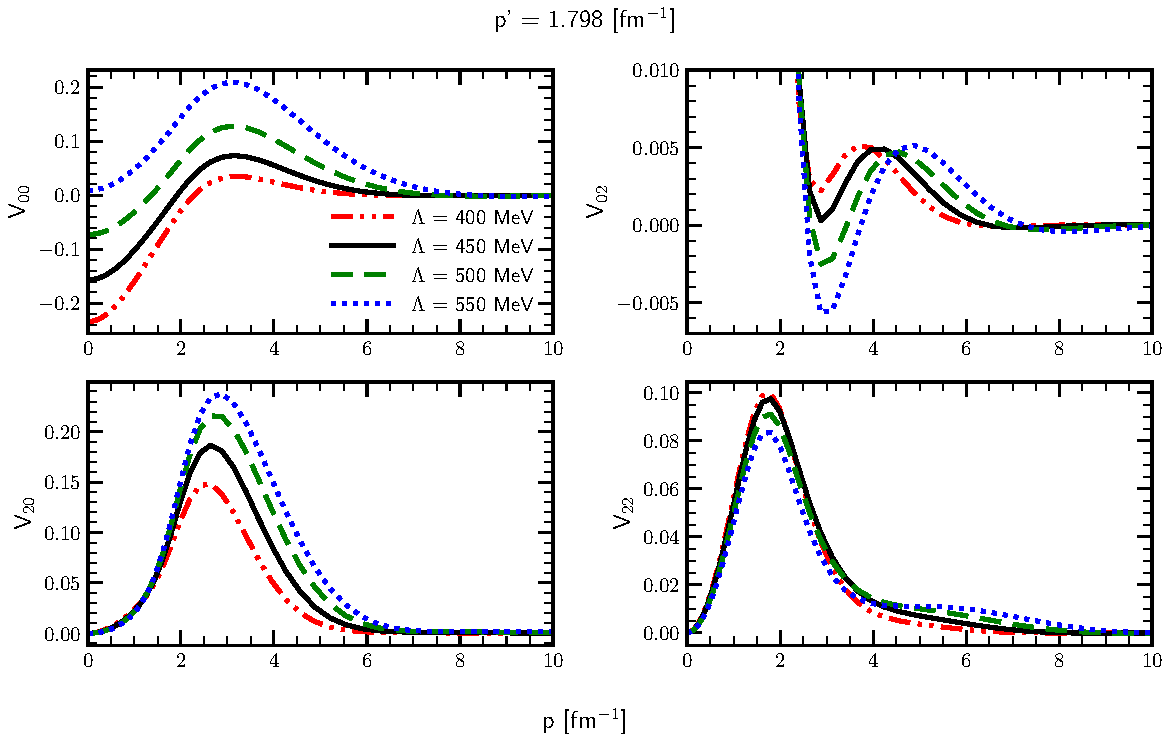
\includegraphics[width=0.95\textwidth]{PlotData/Deuteron/WAVEFUNC/potential_pp1.798.pdf}
    \end{center}
    \caption{Potential components as a function on the momentum $p$ with fixed
    value of the momentum $p'$=1.798 [fm?].
    }
    \label{potential_cutoff}
\end{figure}



The potential may be transformed from coordinate to momentum space (or vice versa),
but it is important at which frame the regularization was performed
and what was a regularization function. That's why there are different 
versions of chiral potential. One is \gls{scs} potential \cite{Epelbaum2014SCS}
and another one is similar, but with regularization applied in momentum space (\gls{sms} potential) \cite{reinkrebs2018}.


\subsection*{Currents}
 
% When it comes to the study of scattering processes on nuclei one has 
% to construct nuclear matrix elements, the crucial part 
% of which is nuclear current. The currents should be consistent with
% the force used


\chapter{Formalism \& numerical methods}
\label{sec:formalism}

Despite the fact that the deuteron problem was solved long time ago, I will describe it briefly 
in order to introduce the notation and formalism. 
With that, for more complex 3N case only slight 
extension will be needed.

In order to calculate any observable for the deuteron photodisintegration,
one has to find a nuclear matrix elements:

% \begin{equation}
%     N^\mu = \langle \Psi_f \vec{P_f} \mid J^\mu(0) \mid \Psi_i \vec{P_i} \rangle =
%     \langle p' (l's')j'm_j't'm_t' \vec{P_f} \mid J^\mu \mid \phi_d m_d \vec{P}_i \rangle, 
%     \label{main}
% \end{equation}
\begin{equation}
    N^\mu = \langle \Psi_{final} \mid J^\mu \mid \Psi_{initial} \rangle, 
    \label{main}
\end{equation}
with two-nucleon wave function of the initial state $\Psi_,
ie. including two- and three- nucleon interaction,{initial}  = \Psi_{deuteron}$;
two-nucleon wave function of the final scattering state $\Psi_{final}$ 
and a four-vector current operator $J^\mu$ which acts between initial and final 
two-nucleon states. In following I describe how to get that quantities.


% $\vec{P_i}$($\vec{P_f}$) is an initial (final) total 2N m\vec{p}omentum.

% One can introduce relative and total momenta for 2 nucleons:

% \begin{eqnarray}
    %     \vec{p} &=& \frac{1}{2} (\vec{p}_1 - \vec{p}_2)\\
    %     \vec{\mathcal{P}} &=& \vec{p}_1 + \vec{p}_2\\
    %     \pvec{p} &=& \frac{1}{2} (\pvec{p}_1^\prime - \pvec{p}_2^\prime)\\
    %     \pvec{\mathcal{P}}^\prime &=& \pvec{p}_1^\prime + \pvec{p}_2^\prime,
    % \end{eqnarray}
    % where $\vec{p}_1$($\pvec{p}_1^\prime$) and $\vec{p}_2$($\pvec{p}_2^\prime$) are
    % initial(final) momenta of the first and second nucleons.
\section{Deuteron bound state}
    \label{sec:deut_bound}

    Let's find a deuteron bound state wave function $\ket{\phi_d}$. 
    The time-independent Schr\"{o}dinger
    equation for two particles expresses as:

    \begin{equation}
        (H_0 + V) \ket{\phi_d}  = E_d \ket{\phi_d},
        \label{shrod_bound}
    \end{equation}
    with a kinetic energy $H_0$ and potential $V$. 
    The kinetic energy $H_0$ can be represented in terms of  relative and total momenta
    of the particles:

    \begin{equation}
        H_0 = \frac{\vec{p}_1^2}{2m_1} + \frac{\vec{p}_2^2}{2m_2} = 
        \frac{\vec{p}^2}{2\mu} + \frac{\vec{\mathcal{P}}^2}{2M}, 
    \end{equation}
    where the relative and total momenta are defined as follows:

    \begin{eqnarray}
        \vec{p} &=& \frac{(m_1\vec{p}_1 - m_2\vec{p}_2)}{m_1 + m_2},\\
        \vec{\mathcal{P}} &=& \vec{p}_1 + \vec{p}_2,
    \end{eqnarray}
    where $M = m_1 + m_2$ is a total mass, $\mu = \frac{m_1m_2}{M}$ is a reduced mass of two nucleons and 
    $\vec{p_i}$ is a momentum of i-th particle.

    Potential $V$ is assumed to depend on the relative degrees of freedom only, so
    \eq{shrod_bound} may be decomposed into two separated equations:

    \begin{eqnarray}
        &\frac{\vec{p}^2}{2\mu} \langle \vec{p} \mid \Psi_{int} \rangle +
        \langle \vec{p} \mid V \mid \Psi_{int} \rangle = 
        (E_d - E)\langle \vec{p} \mid \Psi_{int} \rangle \label{se1}\\
        &\frac{\vec{\mathcal{P}}^2}{2M} \langle \mathcal{P} \mid \Psi \rangle = 
        E\langle \mathcal{P} \mid \Psi \rangle \label{se2},
    \end{eqnarray}
    with $\matrixel{\vec{p},\vec{\mathcal{P}}}{H_0}{\phi_d} = \frac{\vec{p}^2}{2\mu} \braket{\vec{p}}{\Psi_{int}} +
    \frac{\vec{\mathcal{P}}^2}{2M} \braket {\mathcal{P}} {\Psi} $. So $\Psi$ is a component 
    of total wave function, which reflects a deuteron as a single object with momentum $\vec{\mathcal{P}}$
    while $\Psi_{int}$ is an internal wave function describing interaction between nucleons.
    Basis state $\ket{\vec{p}}$  obeys a completeness
    equation:

    \begin{equation}
        \int d^3\vec{p} \ket{\vec{p}} \bra{\vec{p}}   = \mathbb{1}.
        \label{completness}
    \end{equation}

    \eq{se1} is basically the Schr\"{o}dinger equation for a single particle with mass $\mu$
    in potential $V$ 
    and \eq{se2} can be regarded as a Schr\"{o}dinger equation for particle with mass $M$ in 
    a free motion. Assuming that deuteron is at rest ($E = 0$) we can stick 
    to the Eq.(\ref{se1}) only. Using completeness relation (\ref{completness}) we get:

    \begin{equation}
        \frac{\vec{p}^2}{2\mu} \langle \vec{p} \mid \Psi_{int} \rangle +
        \int d \pvec{p} \langle \vec{p} \mid V \mid \pvec{p} \rangle
        \langle \pvec{p} \mid \Psi_{int} \rangle = 
        E_d \langle \vec{p} \mid \Psi_{int} \rangle
        \label{shrod_old}
    \end{equation}

    Working in 3 dimensional space  is difficult, especially numerically,
    so I follow a standard path and introduce the partial-wave decomposed representation (PWD) 
    of the momentum state, adding spin and isospin degrees of freedom in the following form:

    \begin{equation}
        \ket{p \alpha} \equiv \ket{p (ls) j m_j}  \ket{t m_t},
        \label{pwmain}
    \end{equation}
    where quantum numbers l, s, j, t are orbital angular momentum, total spin,
    total angular momentum and total isospin respectively. $m_j$ and $m_t$ are 
    total angular momentum and isospin projections, respectively.


    States $\ket{p (ls) j m_j}$ can be further decomposed to 
    the more basic states than it is in (\ref{pwmain}), separating spin part as 
    
    \begin{equation}
        \ket{p (ls) j m_j} = \sum_{m_l} c(lsj;m_l, m_j\!-\!m_l, m_j) \ket{p l m_l}
        \ket{s~m_j\!-\!m_l}.
        \label{full_decomp}
    \end{equation}

    Spin(isospin) states can be further represented via single-nucleon spin(isospin) states:

    \begin{equation}
        \ket{s m_s} = \sum_{m_1} c(\frac{1}{2}\frac{1}{2}s;m_1, m_s\!-\!m_1, m_s)
        \ket{\frac{1}{2} m_1}
        \ket{\frac{1}{2} m_s\!-\!m_1},
        \label{spin_decomp}
    \end{equation}

    \begin{equation}
        \ket{t m_t} = \sum_{\nu_1} c(\frac{1}{2}\frac{1}{2}t;\nu_1, m_t\!-\!\nu_1, m_t)
        \ket{\frac{1}{2} \nu_1}
        \ket{\frac{1}{2} m_t\!-\!\nu_1}.
        \label{isospin_decomp}
    \end{equation}

    In Eqs.(\ref{full_decomp}) -(\ref{isospin_decomp}),  $c(...)$ are Clebsh-Gordon coefficients.
    Nucleons are spin $\frac{1}{2}$ particles, and we also treat proton and neutron as 
    the same particle in different 
    isospin states, using convention in which isospin $\nu_1 = \frac{1}{2}$ stands for proton and $\nu_1 = -\frac{1}{2}$ is for neutron.

    The states $\mid p l m_l \rangle$ from Eq.(\ref{full_decomp}) are orthogonal
    
    \begin{equation}
        \langle p^\prime l^\prime m_l^\prime \mid p l m_l \rangle = 
        \frac{\delta(p - p^\prime)}{p^2} \delta_{ll^\prime}\delta_{m_l m_l^\prime}
    \end{equation}
    and satisfy the completeness relation:

    \begin{equation}
        \sum_{l=0}^\infty \sum_{m_l=-l}^l \int dp p^2 \mid plm_l \rangle \langle plm_l \mid = \mathbb{1}
    \end{equation}


    Projection of $\bra{\pvec{p}}$ states to $\ket{plm_l}$ leads to

    \begin{equation}
        \braket{\pvec{p}}{plm_l} = 
        \frac{\delta ( \abs{\pvec{p}} - p)}{p^2} Y _{l m_l}(\hat{p}^\prime),
    \end{equation}
    where $Y _{l m_l}(\hat{p}^\prime)$ is a spherical harmonic and 'hat' denotes a unit vector $\hat{X}$ in 
    direction of $\vec{X}$. Thus for the momentum vector:

    \begin{equation}
        \vec{p} \equiv |\vec{p}| \hat{p} \equiv p \hat{p}. 
        \label{hat}
    \end{equation}

    Nucleons are fermions so exchanging them leads to antisymmetry of the
    wave function. In PWD it results in additional requirement on allowed quantum numbers which
    is:

    \begin{equation}
        (-1)^{l+s+t} = -1.
        \label{parity}
    \end{equation}

    In general, nuclear NN force conserves spin, parity and charge so

    \begin{equation}
        \matrixel*{p^\prime\alpha^\prime}{V}{p\alpha} = \delta_{jj'}\delta_{mm'}\delta_{tt'}\delta_{m_tm_{t'}}
        \delta_{ss'}V^{sjtm_t}_{l'l}(p',p)
        \label{conservation}
    \end{equation}
    which introduces restrictions for particular sets of quantum numbers and $\alpha$.
    Strong interaction allows for change of the orbital angular momenta $l = j \pm 1,~l'=j'\pm1$.
    The channels, in which  $l \neq l'$ is allowed,
    are calld a coupled channels and for the deuteron bound state 
    one can find only one such PWD state combination:
    two coupled channels 
    which are commonly denoted as $^3S_1$ and $^3D_1$ (the naming stands for $^{2s+1}l_j$). They correspond 
    to $l=0$ and $l=2$ respectively (with $s = j = 1$ and $t = m_t = 0$). 
    We will call wave functions for these channels as $\phi_l(p)$ with $l=0,2$, such that:

    % Taking into account Eq.(\ref{parity}), one can find only one possible PWD state combination for 
    % the deuteron bound state(under ... experimental evidence): 2 coupled channels for l=0,2; s=1; j=1 and $t = m_t = 0$. 
    % These 2 channels are usually denoted as $^3S_1$ and $^3D_1$ and
    % corresponding wave functions are $\phi_0(p)$ and $\phi_2(p)$:
    
    \begin{equation}
        \phi_l(p) = \bra{p (ls) j m_j}\braket{t m_t}{\Psi_{int}} = \bra{p(l1)1m_d} \braket{00}{\Psi_{int}}; l=0,2.
        \label{deut_waves}
    \end{equation}

    In that new basis Eq.(\ref{shrod_old}) takes a form of two coupled equations:

    \begin{equation}
        \frac{\vec{p}^2}{2\mu} \phi_l(p) +
        \sum_{l^\prime =0,2} \int d p^\prime p^{\prime 2} 
        \bra{p(l1)1m_d} \matrixel{00}{V}{00} \ket{p^\prime(l^\prime1)1m_d}
        % \langle plm_l \mid V \mid p^\prime l^\prime m_l^\prime  \rangle
        \phi_{l^\prime}(p^\prime) = 
        E_d \phi_l(p),
        \label{integral}
    \end{equation}
    for $l=0,2$. In case one does not have a matrix elements for the potential 
    $\langle plm_l \mid V \mid p^\prime l^\prime m_l^\prime  \rangle$ in analytical form,
    but only numerical values for some grid of points are given, 
    there is still one complication in the Eq.(\ref{integral}) - integration, which has to be discretized.
    In order to get rid of the integral I use a Gaussian quadrature 
    method of numerical integration \cite{jacobi1826ueber}.
    It allows me to replace an integral by the weighted sum:
        $\int_a^b f(x)dx = \sum_{i=1}^n \omega_i f(x_i)$
    In current work I used $N=72$ points in the interval from $0$ to \SI{50}{fm^{-1}}. 
    Using this method, Eq.(\ref{integral}) becomes  

    
    \begin{equation}
        \frac{p_i^2}{2\mu} \phi_l(p_i) +
        \sum_{l^\prime =0,2}\sum_{j =0}^{N_P}  \omega_j p^{2}_j 
        \bra{p_i(l1)1m_d} \matrixel{00}{V}{00} \ket{p_j(l^\prime1)1m_d}
        % \langle p_jlm_l \mid V \mid p^\prime_j l^\prime m_l^\prime  \rangle
        \phi_{l^\prime}(p_j) = 
        E_d \phi_l(p_i).
        \label{integral2}
    \end{equation}

    In practical computations, the same grid points $p_i$ and $p_j$ are used in order
    optimize computational time. 
    I solve this equation as an eigenvalue problem $M\Psi = E_d \Psi$ and
    in that way
    find simultaneously wave function values in grid of $p$ points and The binding energy $E_d$. 
    The binding energy $E_d$ calculated with potentials at different chiral orders 
    is presented in Fig.~\ref{bind}.

    \begin{figure}[h]
        \begin{center}
            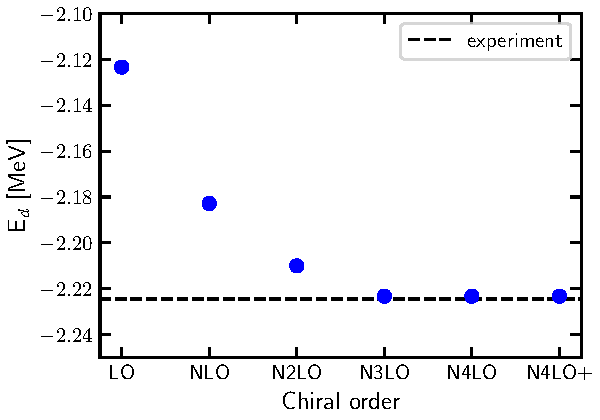
\includegraphics[width=0.65\textwidth]{Figures_De/Binding_energy.pdf}
        \end{center}
        \caption{Deuteron binding energy calculated using the chiral \gls{sms} potential
        at different chiral orders as a mean value over all cutoffs.
        % Error bands represent a spread the calculated binding energy with respect to
        % the cutoff parameter $\Lambda$ (minimal and maximal values).
        Experimental data is taken from \cite{VANDERLEUN1982261}.}
        \label{bind}
    \end{figure}

    An example of such wave functions is demonstrated in \fig{wave_func}. The left panel demonstrate
    a wave function for $l=0$ - $^3S_1$ while the right one - for $l=2$ - $^3D_1$. Both 
    plots consist of the curves for different cutoff values and using the chiral \gls{sms} potential at \gls{n4lo+}.
    The small deviation between lines show that cutoff dependence is rather weak at this stage
    and further discrepancies connected to the value of $\Lambda$ may appear in other components
    of nuclear matrix elements.  

    \begin{figure}[h]
        \begin{center}
            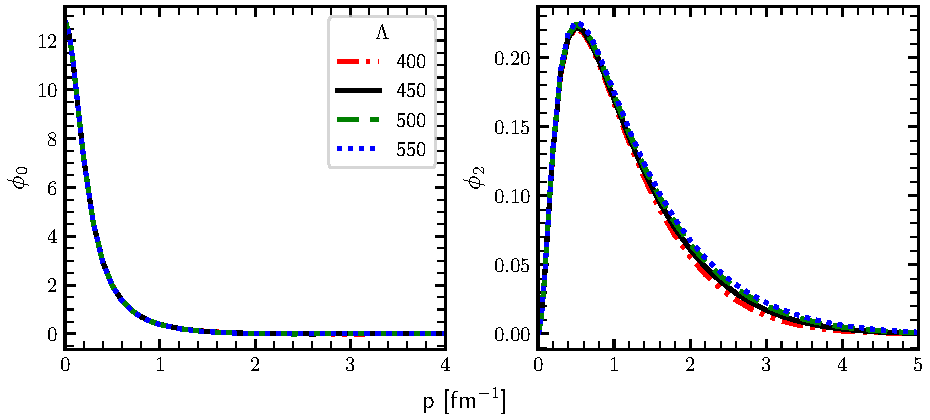
\includegraphics[width=0.85\textwidth]{Figures_De/Wave_function_cutoff.pdf}
        \end{center}
        \caption{The deuteron wave function $\phi_l$ for l=0 ($^3S_1$ partial wave)(left) and l=2 ($^3D_1$) (right).
        Each curve shows results obtained with different values of the cutoff parameter $\Lambda$. 
        The chiral \gls{sms} potential at \gls{n4lo+} was used.}
        \label{wave_func}
    \end{figure}

\section{2N scattering state}

% \subsection{The Lippmann-Schwinger equation}
    % Let us consider a two-nucleon scattering state $\mid \Psi _f \rangle$, It fulfills
    % a Schr\"{o}dinger equation

    % \begin{equation}
    %     (H_0 + V) \mid \Psi _f \rangle = E \mid \Psi _f \rangle,
    %     \label{schrod_scatt}
    % \end{equation}
    % with $H_0 = \frac{\vec{p}^2}{m}$ and $E > 0$.

    % Solution to the Eq.(\ref{schrod_scatt}) can be presented in the form:

    % \begin{equation}
    %     \mid \Psi _f \rangle = \mid \Psi _0 \rangle + \frac{1}{E - H_0 + i \epsilon} V \mid \Psi _f \rangle
    % \end{equation}

    I work in the time-independent formulation of the scattering process.
    In such a case the Hamiltonian is:

    \begin{equation}
        H = H_0 + V,
    \end{equation}
    where again $H_0$ is a kinetic energy operator, $H_0 = \frac{\vec{p}^2}{2m}$, 
    and $V$ is a nucleon-nucleon interaction.
    For a free particle motion, $V$ will be absent and we will denote a corresponding energy eigenstate as
    a free particle state $\ket{\vec{p}\,}$.
    The scattering state $\ket{\psi}$ fulfills similar Schr\"{o}dinger equation as 
    $\ket{\vec{p}\,}$, with the same energy eigenvalue,
    but with the presence of the potential:
    
    % , the eigenstate will differ from $\ket{\phi_l}$,
    % but in case of elastic scattering (which we are interested in) the energy eigenvalue $E$ should be the same.

    % So these two states fulfill Schr\"{o}dinger equations for such scattering process:

    \begin{equation}
        \begin{cases}
            H_0 \ket{\vec{p}\,} &= E \ket{\vec{p}\,}, \\
            (H_0 + V) \ket{\psi} &= E \ket{\psi}.
        \end{cases}
        \label{system}
    \end{equation}

    We are interested in solution for \eq{system}, so that 
    $\ket{\psi} \rightarrow \ket{\vec{p}\,}$ as $V \rightarrow 0$
    and both $\ket{\psi}$ and $\ket{\vec{p}\,}$ have the same energy eigenvalues E.
    As we have scattering process, the energy spectra for both operators $H_0$ and $H_0 + V$
    are continuous. 

    From \eq{system} it follows that

    \begin{equation}
        \ket{\psi} = \frac{1}{E - H_0}V \ket{\psi} +  \ket{\vec{p}\,},
        \label{psieq}
    \end{equation}
    % where $\mid \vec{p} \rangle$ is a solution to the
    % free-particle Schr\"{o}dinger equation
    % \begin{equation}
    %     H_0 \ket{\vec{p}} =  E  \ket{\vec{p}},
    % \end{equation}
    % with same energy eigenvalue\cite{Sakurai}.
    % was added artificially in order to satisfy a criterion mentioned above 
    % and following the logic from . 
    % In addition, it 
    which guarantees that
     application of the operator $(E -H_0)$ to the 
    \eq{psieq} results in the second equation from the set (\ref{system}).
    % Also, \eq{psieq} for $V \rightarrow 0$ becomes $\mid \psi \rangle = \mid \vec{p} \rangle$


    In order to deal with a singular operator $\frac{1}{E - H_0}$ in \eq{psieq}, the well-known
    technique is used to make such an operator complex by adding small imaginary number to the denominator
    so \eq{psieq} becomes
    % making it  $\frac{1}{E + i\epsilon - H_0}$.

    \begin{equation}
        \ket{\psi} = G_0(E \pm i\epsilon)V \mid \psi \rangle +  \mid \vec{p} \rangle,
        \label{lse}
    \end{equation}
    where $G_0$ is a free propagator:

    \begin{equation}
        G_0(z) = \frac{1}{z - H_0}.
        \label{g0}
    \end{equation}

    Solution with $G_0(E - i\epsilon)$ corresponds to the incoming spherical wave,
    while $G_0(E + i\epsilon)$ - to the outgoing one. Since we are interested in the final scattering
    state, only the $(+)$ sign survives.
    
    Eq.~(\ref{lse}) is known as the Lippmann-Schwinger equation (LSE).
    Defining the transition operator $t$:

    \begin{equation}
        t \ket{\vec{p}} = V \ket{\psi}
        \label{t-op}
    \end{equation}
    we can rewrite it as 

    \begin{equation}
        \ket{\psi} = (1 + G_0(E + i\epsilon) t)  \ket {\vec{p}}.
        \label{psi_toper}
    \end{equation}

    With substitution of \eq{lse} into \eq{t-op} we can find
    an explicit form of the $t$ operator:

    \begin{eqnarray}
        t \ket{\vec{p}} = V G_0(E + i\epsilon)V \mid \psi \rangle +  V \mid \vec{p} \rangle = \nonumber\\
        = V G_0(E + i\epsilon) t \ket{\vec{p}} +  V \mid \vec{p} \rangle
        \label{top2}
    \end{eqnarray}

    Getting rid off the initial state $\ket{\vec{p}}$ in the \eq{top2} we can get the LSE
    for the transition operator in the iterative form:

    \begin{eqnarray}
        t = V + V G_0 t = \nonumber\\
        = V + V G_0 V + V G_0 V G_0V + ...,
        \label{lse_gen}
    \end{eqnarray}
    which constitutes an infinite series of subsequent NN interactions and free propagators of nucleons.

    In the partial-wave representation, the LSE \eq{top2} expresses as:
    \begin{multline}
        \bra{p^\prime (l^\prime s^\prime)j'm_{j'}}\matrixel{t' m_{t'}}{t(E)}{t m_t}\ket{p (l s)jm_{j}} = 
        \bra{p^\prime (l^\prime s^\prime)j'm_{j'}}\matrixel{t' m_{t'}}{V}{t m_t}\ket{p (l s)jm_{j}} + \\
        +\sum_{\alpha^{\prime\prime}} \int_0^\infty dp^{\prime \prime} p^{\prime \prime 2}
        \bra{p^\prime (l^\prime s^\prime)j'm_{j'}}\matrixel{t' m_{t'}}{V}
        {t'' m_{t''}}\ket{p'' (l'' s'')j''m_{j''}} \\
        \cross \frac{1}{E + i\epsilon - p^{\prime \prime 2}/m}
        \bra{p'' (l'' s'')j''m_{j''}}\matrixel{t'' m_{t''}}{t(E)}{t m_t}\ket{p (l s)jm_{j}},
        \label{lse_pwd}
    \end{multline}
    which after using symmetries of potential matrix elements (\ref{conservation}) reduces to
    
    \begin{multline}
        \matrixel{p^\prime (l^\prime s^\prime)jt}{t(E)}{p(ls)jt} = 
        \matrixel{p^\prime (l^\prime s)jt}{V}{p(ls)jt} + \\
        +\sum_{l^{\prime\prime}} \int_0^\infty dp^{\prime \prime} p^{\prime \prime 2}
        \matrixel{p^\prime (l^\prime s)jt}{V}{p^{\prime\prime}(l^{\prime\prime} s)jt} \\
        \cross \frac{1}{E + i\epsilon - p^{\prime \prime 2}/m}
        \matrixel{p^{\prime \prime} (l^{\prime \prime} s)jt}{t(E)}{p(l s)jt}.      
        \label{lse_pwd_reduced}
    \end{multline}

    I solve \eq{lse_pwd_reduced} numerically, which again requires discretisation
    and therefor leads to set of linear equations.
    Finally, using \eq{psi_toper} and denoting the momentum state of two nucleons
    with spin projections $m_p$ and $m_n$ as $\bra{\phi m_p m_n}$, we can write \eq{main} as
    
    \begin{equation}
        N^\mu = \bra{\phi m_p m_n} (1 + G_0(E + i\epsilon) t) J^\mu(0) \mid \Psi_{deuteron} \rangle
        \label{main_top}
    \end{equation}

    %TODO: rewrite everything in \phi m_d m_n
    
\section{3N bound state}

    The 3N bound state is described by the Schr\"{o}dinger equation for 3N system,
    ie. including two- and three- nucleon interaction,
    and its total wave function obeys the following equation:

    \begin{equation}
        \ket{\Psi} = G_0(E+i\epsilon)\sum_{j=1}^3 (V_j + V_4^j) \ket{\Psi},
        \label{psi3_total}
    \end{equation}
    where $G_0$ is a 3N free propagator as in \eq{g0}, $V_j$ - is a two-body potential
    acting between nucleons $k$ and $l$ (j, k and l - numerate nucleons, $j,k,l \in {1,2,3}$ and $j \neq k \neq l$),
    $V_4^j$ is a component of three-body potential $V_4 = \sum_{j=1}^3 V_4^j$
    symmetrical under exchange of nucleons $k$ and $l$,
    and $E$ - is a 3N binding energy.

    \eq{psi3_total} can be split into three independent equations for
    so-called Faddeev components $\ket{\psi_j}$

    \begin{equation}
        \ket{\Psi} = \sum_{j=1}^3 \ket{\psi_j},
        \label{faddeev_comps}
    \end{equation}
    which fulfills separately

    \begin{equation}
        \ket{\psi_j} = G_0(E+i\epsilon)(V_j + V_4^j) \ket{\Psi}.
        \label{psi3_component}
    \end{equation}

    Next, I introduce a permutation operator P, which is a combination
    of operators $P_{jk}$:
    
    \begin{equation}
        P = P_{12}P_{23} + P_{13}P_{32}.
        \label{permutation}
    \end{equation}

    The operator component $P_{jk}$ acting on the state interchange the momenta and  
    quantum numbers of the nucleons $j$ and $k$.

    Using definitions \ref{permutation} and \ref{faddeev_comps},
    one can rewrite \eq{psi3_component} as:

    \begin{equation}
        \ket{\psi_j} = G_0(E+i\epsilon)t_j P \ket{\psi_j} + 
        (1 + G_0(E+i\epsilon)t_j)G_0(E+i\epsilon)V_4^j(1+P)\ket{\psi_j},
        \label{fadeed_lse}
    \end{equation}
    where $t_j$ is a two-body t-operator which obeys \eq{top2} for corresponding 
    two-body potential $V_j$. I solve \eq{fadeed_lse} numerically to find $\ket{\psi_j}$
    and the binding energy $E$. To do that, I perform PWD again.

The partial wave representation of the \eq{fadeed_lse} is obtained using
following 3N states:

\begin{equation}
    \ket{p,q,\alpha_{J,M_J}} = \ket{p,q,(ls)j, (\lambda, \frac{1}{2})I(jI)JM;(t\frac{1}{2})TM_T}_1,
    \label{3N_PW}
\end{equation}
where index 1 states the choice of the Jacobi momenta, such that $p$ is a relative momentum of the nucleons 2 and 3.
Values l, s and j are quantum numbers in the two-body subsystem consisted of nucleons 2 and 3. $\lambda$ is the 
orbital angular momentum with respect to the c.m. of the particles 2 and 3,
of the first particle which spin is $\frac{1}{2}$
and $I$ is its total angular momentum.
$J$ and $M_J$ are the total angular momentum of the 3N system and its projection on the z-axis respectively.
$t$ is a total isospin of the 2-3 subsystem whereas $T$ and $M_T$ are the total isospin of the 3N system and its projection on the z-axis, respectively.  

% Using states defined in \eq{3N_PW}, we can write a partial-wave representation of the \eq{fadeed_lse}:
% \begin{equation}
%     \begin{aligned}
%         \left\langle p, q, \alpha_{J, M_J}\right. & \left|\psi_i\right\rangle=\frac{1}{E-\frac{p^2}{m}-\frac{3 q^2}{4 m}+i \epsilon}[ \\
%         & \sum_{\alpha^{\prime}, \alpha^{\prime \prime}} \int_0^{\infty} d q^{\prime \prime} q^{\prime \prime 2} \int_{-1}^1 d x t_{\alpha, \alpha^{\prime}}^{+}\left(p, \pi_1\left(q, q^{\prime \prime}, x\right), E-\frac{3 q}{4 m}\right) \\
%         * & \frac{\tilde{G}_{\alpha^{\prime}, \alpha^{\prime \prime}}\left(q^{\prime}, q^{\prime \prime}, x\right)}{\pi_1^{l^{\prime}} \pi_2^{l^{\prime \prime}}}\left\langle\pi_2, q^{\prime \prime}, \alpha_{J^{\prime \prime}, M_{J^{\prime \prime}}^{\prime \prime}} \mid \psi_i\right\rangle \\
%         +\quad & \sum_{\alpha^{\prime \prime}} \int_0^{\infty} d p^{\prime \prime} p^{\prime \prime 2} \int_0^{\infty} d q^{\prime \prime} q^{\prime \prime 2} V_{\alpha, \alpha^{\prime \prime}}^4\left(p, q, p^{\prime \prime}, q^{\prime \prime}\right)\left\langle p^{\prime \prime}, q^{\prime \prime}, \alpha_{J^{\prime \prime}, M_{J^{\prime \prime}}^{\prime \prime}} \mid \psi_i\right\rangle \\
%         +\quad & \sum_{\alpha^{\prime}, \alpha^{\prime \prime}} \int_0^{\infty} d q^{\prime} q^{\prime 2} \int_0^{\infty} d q^{\prime \prime} q^{\prime \prime \prime} \int_{-1}^1 d x V_{\alpha, \alpha^{\prime}}^4\left(p, q, \pi_1\left(q^{\prime}, q^{\prime \prime}, x\right), q^{\prime}\right) \\
%         +\quad & \frac{\tilde{G}_{\alpha^{\prime}, \alpha^{\prime \prime}}\left(q^{\prime}, q^{\prime \prime}, x\right)}{\pi_1^{l^{\prime}} \pi_2^{l^{\prime \prime}}}\left\langle\pi_2, q^{\prime \prime}, \alpha_{J^{\prime \prime}, M_{J^{\prime \prime}}^{\prime \prime}} \mid \psi_i\right\rangle\\
%         & +\sum_{\alpha^{\prime}, \alpha^{\prime \prime}} \int_0^{\infty} d p^{\prime} p^{\prime 2} \int_0^{\infty} d p^{\prime \prime} p^{\prime \prime 2} \int_0^{\infty} d q^{\prime \prime} q^{\prime \prime 2} t_{\alpha, \alpha^{\prime}}^{+}\left(p, p^{\prime}, E-\frac{3 q^2}{4 m}\right) \frac{1}{E-\frac{p^{\prime 2}}{m}-\frac{3 q^2}{4 m}+i \epsilon} \\ & \text { * } \quad V_{\alpha^{\prime}, \alpha^{\prime \prime}}^4\left(p^{\prime}, q, p^{\prime \prime}, q^{\prime \prime}\right)\left\langle p^{\prime \prime}, q^{\prime \prime}, \alpha_{J^{\prime \prime}, M_{J^{\prime \prime}}}^{\prime \prime} \mid \psi_i\right\rangle \\ & +\sum_{\alpha^{\prime}, \alpha^{\prime \prime}, \alpha^{\prime \prime \prime}} \int_0^{\infty} d p^{\prime} p^{\prime 2} \int_0^{\infty} d q^{\prime \prime} q^{\prime \prime 2} \int_0^{\infty} d q^{\prime} q^{\prime 2} \int_{-1}^1 d x t_{\alpha, \alpha^{\prime}}^{+}\left(p, p^{\prime}, E-\frac{3 q^2}{4 m}\right) \\ & \text { * } \frac{1}{E-\frac{p^{\prime 2}}{m}-\frac{3 q^2}{4 m}+i \epsilon} V_{\alpha^{\prime}, \alpha^{\prime \prime \prime}}^4\left(p^{\prime}, q, \pi_1\left(q^{\prime}, q^{\prime \prime}, x\right), q^{\prime}\right) \\ & \left.* \quad \frac{\tilde{G}_{\alpha^{\prime \prime \prime}, \alpha^{\prime \prime}}\left(q^{\prime}, q^{\prime \prime}, x\right)}{\pi_1^{l^{\prime \prime \prime}} \pi_2^{l^{\prime \prime}}}\left\langle\pi_2, q^{\prime \prime}, \alpha_{J^{\prime \prime}, M_{J^{\prime \prime}}}^{\prime \prime} \mid \psi_i\right\rangle\right] \text {, } \\ & 
%     \end{aligned}
% \end{equation}

% where

% \begin{equation}
%     V_{\alpha, \alpha^{\prime}}^4\left(p, q, p^{\prime}, q^{\prime}\right) \equiv\left\langle p, q, \alpha_{J, M_J}\left|V_4^{(1)}\right| p^{\prime}, q^{\prime}, \alpha_{J^{\prime}, M_{J^{\prime}}}^{\prime}\right\rangle
% \end{equation}
    

\section{3N scattering state}

    Let us
    introduce an asymptotic state $\ket{\Phi^{3N}_j}$ describing a free motion
    of three nucleons ${j,k,l}$ with particles $k$ and $l$ 
    having relative momentum $\vec{p}$
    and particle $j$ moving with momentum $\vec{q}$ relatively to the 
    center of mass $(k-l)$:
    
    \begin{equation}
        \ket{\Phi^{3N}_j} \equiv \frac{1}{\sqrt{2}}(1 - P_{kl})
        \ket{\vec{p}(kl)\vec{q}(j)}.\\
    \end{equation}

    The Jacobi momenta $\vec{p}$ and $\vec{q}$ build the total energy of three
    nucleons in the 3N-c.m. system:
    
    \begin{equation}
        E_{3N} = \frac{|\vec{p}|^2}{m} + \frac{3 |\vec{q}|^2}{4m}.
    \end{equation}
    
    Using a free propagator $G(E_{3N} - i\epsilon)$ we can come up with
    the total 3N scattering state

    \begin{equation}
        \ket{\Psi^{(-)}}^{3N} = \frac{1}{\sqrt{3}} \sum_j\ket{\Psi^{(-)}_j}^{3N},  
    \end{equation}
    where auxiliary scattering states $\ket{\Psi^{(-)}_j}^{3N}$ are defined as \cite{Glockle1983} 

    \begin{eqnarray}
        \ket{\Psi^{(-)}_j}^{3N}  &\equiv& \lim_{\epsilon \rightarrow 0}
        i \epsilon G(E_{3N} - i\epsilon)\ket{\Phi^{3N}_j}.
    \end{eqnarray}

    The state $\ket{\Psi^{(-)}_j}^{3N}$ together with the state $\ket{\Phi^{3N}_j}$ fulfills an equation \cite{Glockle1983}

    \begin{equation}
        \left|\Psi_j^{(-)}\right\rangle^{3 N}=\left|\Phi_j^{3 N}\right\rangle+
        G_0\left(V_1+V_2+V_3+V_4\right)\left|\Psi_j^{(-)}\right\rangle^{3 N}.
    \end{equation}

    Defining the antysymmetrized Faddeev components, and using index "$i$" instead of "$j$"

    \begin{equation}
        \left|F_i^0\right\rangle \equiv G_0\left(V_i+V_4^{i}\right)(1+P)\left|\Psi_i^{(-)}\right\rangle^{3 N}
        \label{faddeev_3n}
    \end{equation}
    we obtain a 3N scattering wave function as:

    \begin{equation}
        \begin{aligned}
            \left|\Psi^{(-)}\right\rangle^{3 N} & =\frac{1}{\sqrt{3}}\left(\sum_{i=1}^3\left|\Phi_i^{3 N}\right\rangle+G_0\left(V_1+V_2+V_3+V_4\right) \sum_{i=1}^3\left|\Psi_i^{(-)}\right\rangle^{3 N}\right) \\
            & =\frac{1}{\sqrt{3}}\left(\sum_{i=1}^3\left|\Phi_i^{3 N}\right\rangle+\sum_{i=1}^3\left|F_i^0\right\rangle\right)
            =\frac{1}{\sqrt{3}}(1+P)\left(\left|\Phi_1^{3 N}\right\rangle+\left|F_1^0\right\rangle\right) .
        \end{aligned}
        \label{3n_scat_psi}
    \end{equation}

    In this case the nuclear matrix element 
    $N_\mu^{3 N} = \matrixel{\Psi^-}{j^\mu}{\psi_i}$ 
    (with $\ket{\psi_i}$ being the Faddeev component of the 3N bound state (\ref{faddeev_comps})) is
    \cite{GLOCKLE_report_1996, skibinski_prc_2003} \tmp{???}:

    \begin{equation}
        \begin{aligned}
            N_\mu^{3 N} & =\frac{1}{\sqrt{3}}\left\langle\Phi_1^{3 N}\left|(1+P) j_\mu\right| \Psi_i\right\rangle+\frac{1}{\sqrt{3}}\left\langle\Phi_1^{3 N}\left|t_1^{+} G_0^{+}(1+P) j_\mu\right| \Psi_i\right\rangle \\
            & +\frac{1}{\sqrt{3}}\left\langle\Phi_1^{3 N}\left|t_1^{+} G_0^{+} P\right| U_\mu\right\rangle+\frac{1}{\sqrt{3}}\left\langle\Phi_1^{3 N}|P| U_\mu\right\rangle,
            \end{aligned}
        \label{3n_matrix}
    \end{equation}
    where $ U_\mu$ fulfills the
    following equation:

    \begin{equation}
        \begin{aligned}
            \left|U_\mu\right\rangle & =\left[t_1^{+} G_0^{+}+\frac{1}{2}(1+P) V_4^{(1)} G_0^{+}\left(1+t_1^{+} G_0^{+}\right)\right](1+P) j_\mu\left|\Psi_i\right\rangle \\
            & +\left[t_1^{+} G_0^{+} P+\frac{1}{2}(1+P) V_4^{(1)} G_0^{+}\left(1+t_1^{+} G_0^{+}\right) P\right]\left|U_\mu\right\rangle.
            \end{aligned}
        \label{u_mu}
    \end{equation}

    \eq{u_mu} is being solved numerically in PWD. The techniques applied closely resemble those presented in \cite{GLOCKLE_report_1996} for N-d elastic scattering.



\section{Nd scattering state}
\label{nd_state}

    Analogously to the bound state, one can express a nucleon-deuteron
    scattering state
    using a permutation operator \eq{permutation}.

    \begin{equation}
        \ket{\Psi^{(-)}}^{Nd} = \frac{1}{\sqrt{3}}\sum_j\ket{\Psi^{(-)}_j}^{Nd}    
    \end{equation}

    Further a scattering state $\ket{\Psi^{(-)}_j}^{Nd}$ can be expressed
    in terms of asymptotic state $\ket{\Phi^{Nd}_j}$, in which particles
    k and l form a deuteron and the third particle (nucleon j)
     propagates freely with a relative momentum $\vec{q}_0$ with 
    respect to the deuteron:

    \begin{eqnarray}
        \ket{\Psi^{(-)}_j}^{Nd} &\equiv& \lim_{\epsilon \rightarrow 0} 
        i \epsilon G(E_{Nd} - i\epsilon)\ket{\Phi^{Nd}_j}\\
        \ket{\Phi^{Nd}_j} &\equiv& \ket{\Phi_{d(k,l)}}\ket{\vec{q}_0},
    \end{eqnarray}
    where $\ket{\Phi_{d(k,l)}}$ is a deuteron wave function and 
    $\ket{\vec{q}_0}$ - a free particle state and $G(t)$ is 
    a free propafator of N-d pair. 
    $E_{Nd}$ is a total energy of the N-d system:

    \begin{equation}
        E_{Nd} = E_d + \frac{3 |\vec{q}_0|^2}{4m},
    \end{equation}
    where $E_d$ is the deuteron binding energy and $m$ denotes the nucleon mass. 

    $\ket{\Psi^{(-)}}^{Nd}$ can be expressed by the Faddeev components

    \begin{equation}
        \ket{\Psi^{(-)}}^{Nd} = \frac{1}{\sqrt{3}} (1+P) \ket{F_1},
    \end{equation}
    where 
    
    \begin{equation}
        \ket{F_1} = \ket{\phi_1^{Nd}} G_0 (\nu_1 + \nu_2 + \nu_3 + \nu_4) 
        \sum_{j=1}^3 \ket{\Psi_j^{(-)}}^{Nd}.
    \end{equation}

    The nuclear matrix element $N_\mu^{Nd} = ^{Nd} \matrixel{\Psi^{-}}{j_\mu}{\Psi_i}$ 
    (with $\Psi_i$ - bound state) is now \cite{GLOCKLE_report_1996, skibinski_prc_2003} \tmp{???}:

    \begin{equation}
        N_\mu^{N d}=\frac{1}{\sqrt{3}} \matrixel{\Phi_1^{N d}}{(1+P) j_\mu}{\Psi_i}
        +\frac{1}{\sqrt{3}} \matrixel{\Phi_1^{N d}}{P}{U_\mu}
    \end{equation}
    with $U_\mu$ being a solution to

    \begin{eqnarray}
       \ket{U_\mu} &=& \left[t_1^{+} G_0^{+}+\frac{1}{2}(1+P) V_4^{(1)} G_0^{+}\left(1+t_1^{+} G_0^{+}\right)\right](1+P) j_\mu \ket{\Psi_i} + \nonumber\\
       &+& \left[t_1^{+} G_0^{+} P+\frac{1}{2}(1+P) V_4^{(1)} G_0^{+}\left(1+t_1^{+} G_0^{+}\right) P\right]\ket{U_\mu}
       \label{u_mu_nd}
    \end{eqnarray}

    \eq{u_mu_nd} is being solved numerically in a same way as \eq{u_mu}, namely applying
    PWD as it is described in \cite{GLOCKLE_report_1996}.


    \section{Nuclear electromagnetic current}
    \label{sec_current}
    
    % The use of nuclear currents in scattering experiments is essential for understanding the structure of the nucleus and
    % the interactions between its constituent nucleons. Advances in theoretical and experimental techniques have allowed
    % for more precise measurements of these currents and have provided insights into
    % the fundamental properties of the nucleus.

    % The nuclear one-body current is constructed based on the electromagnetic current for a Dirac particle. To account
    % for the extended structure of nucleons, form factors are introduced. Since we use nonrelativistic wave functions, we need to use nonrelativistic currents.    
    % \tmp{????????????????????????????????????????????????????}
    The electromagnetic current operator for 2N (3N) system is constructed 
    from the one- and many-body currents:
    
    \begin{equation}
        j_\mu = j_\mu^1 + j_\mu^2 (+ j_\mu^3).
        \label{j_mu_gen}
    \end{equation}

    In \eq{j_mu_gen} $j_\mu^n$ is a contribution from the interaction between photon and 
    $n$ nucleons ($j_\mu^3$ is presented in 3N system only)
    and ($j_\mu^1$) is a sum of interactions with each nucleon in the system. 
    % For 2N:

    % \begin{equation}
    %     j_\mu^1 = j_\mu^1(1) + j_\mu^1(2),
    % \end{equation}
    % where $j_\mu^1(i)$ is an interaction of photon with $i$-th nucleon.


    Regarding the photodisintegration process, only a \gls{snc} is used, so I stick to its definition here.. 
    In the Hamiltonian framework, the nucleons are constrained to lie on the mass shell.
    The general current expression for a
    single nucleon at the spacetime point zero, denoted as $j^1_\mu(0)$, is computed between the initial nucleon momentum
    $p \equiv\left(p_0=\sqrt{M_N^2+\vec{p}\,^2}, \vec{p}\right)$
    and the final momentum
    $p^{\prime} \equiv\left(p_0^{\prime}=\sqrt{M_N^2+\pvec{p}^{2}}, \pvec{p}\right)$. This computation yields the following expression:

    \begin{equation}
        \begin{aligned}
        \matrixel{\pvec{p}} {j^1_\mu(0)} {\vec{p}} & =& \bar{u}\left(\pvec{p} s^{\prime}\right)\left(\gamma^\mu F_1+i \sigma^{\mu \nu}\left(p^{\prime}-p\right)_\nu F_2\right) u(\vec{p} s) \\
        & =&\bar{u}\left(\pvec{p} s^{\prime}\right)\left(G_M \gamma^\mu-F_2\left(p^{\prime}+p\right)^\mu\right) u(\vec{p} s) .
        \end{aligned}
        \label{current_general}       
    \end{equation}
    
    In the above equation,
    ie. including two- and three- nucleon interaction, the symbols $u(\vec{p} s)$ represent Dirac spinors
    for particle having momentum $\vec{p}$ and spin $s$, 
    $F_1$ and $F_2$ are the Dirac and Pauli form factors of the nucleon, respectively, and $G_M \equiv F_1+2 M_N F_2$ denotes the magnetic form factor of the nucleon. The proton charge $e$ is extracted from the matrix element. In this thesis, only the nonrelativistic limit of \eq{current_general} is considered, which leads to well-known expressions for the operators for the current:


    \begin{align}
        % \begin{array}{r}
            \matrixel*{\pvec{p}} {j^1_0} {\vec{p}} &=\left(G_E^p \Pi^p+G_E^n \Pi^n\right), \\
            \matrixel{\vec{p}} {\vec{j^1}} {\vec{p}} &=\frac{\vec{p}+\pvec{p}}{2 M_N}\left(G_E^p \Pi^p+G_E^n \Pi^n\right)+\frac{i}{2 M_N}\left(G_M^p \Pi^p+G_M^n \Pi^n\right) \vec{\sigma} \times\left(\pvec{p}-\vec{p}\right) .
        % \end{array}
        \label{snc_formfact}
    \end{align}

    The electric form factor, denoted as $G_E$, is defined as,
    $G_E \equiv F_1+\frac{\left(p^{\prime}-p\right)^2}{2 M_N} F_2$ and 
    represents the neutron (n) and proton (p) form factors.
    Both electric and magnetic form factors, $G_E$ and $G_M$, are normalized as:

    \begin{equation}
        \begin{aligned}
        G_E^n(0) & =0 \\
        G_E^p(0) & =1 \\
        G_M^n(0) & =-1.913 \\
        G_M^p(0) & =2.793
        \end{aligned}
    \end{equation}

    The above values correspond to nucleons with point-like characteristics. While all the form factors depend on the squared
    four-momentum transfer $\left(p^{\prime}-p\right)^2$, in the nonrelativistic regime, it is common to use the squared
    three-momentum transfer $-\left(\pvec{p}-\vec{p}\right)^2$ or even set it to zero for interactions involving
    real photons. Numerous authors have investigated the properties of electromagnetic nucleon form factors through
    theoretical and experimental approaches, as discussed in \cite{Arrington_2007, JOURDAN1999513c}.
    $\Pi^p$ ($\Pi^n$) in \eq{snc_formfact} is a proton (neuteron) isospin projection operator.

    The two-nucleon current contribution is in that work taken into account via Siegert approach \cite{Siegert, GolakKamad2000_ExplDescr, Golak2005}.
    In order to do that we break down the single nucleon current matrix elements into multipole components and 
    represent some of the electric multipoles using the Coulomb multipoles,
    which arise from the single nucleon charge density operator \cite{Golak2005}.
    This is acceptable because, in low-energy situations, contributions from many nucleons to the nuclear charge density are typically insignificant.
    We then obtain the rest of the electric multipoles and all of the magnetic multipoles exclusively from the single nucleon current operators.

    In 3N system we have following componnents of the \gls{snc}:

    \begin{align}
        % \begin{aligned}
            \matrixel**{\pvec{p}, \pvec{q}}{j_0^1}{\vec{p}, \vec{q}} 
            & =\int d \ppvec{p} d \ppvec{q}
            \matrixel**{\pvec{p}, \pvec{q}}{\frac{1}{2}\left(1+\tau(1)_z\right) F_1^p+\frac{1}{2}\left(1-\tau(1)_z\right) F_1^n}{\ppvec{p}, \ppvec{q}}\nonumber\\
            &\braket{\ppvec{p}, \ppvec{q}-\frac{2}{3} \vec{Q}}{\vec{p}, \vec{q}} \\
            \matrixel**{\pvec{p}, \pvec{q}}{j_{ \pm}^{1, \text { conv }}} {\vec{p}, \vec{q}} 
            & =\frac{1}{m} \int d \ppvec{p} d \ppvec{q}
            \bra{\pvec{p}, \pvec{q}}\left[\frac{1}{2}\left(1+\tau(1)_z\right) F_1^p+\frac{1}{2}\left(1-\tau(1)_z\right) F_1^n \right] q_{ \pm}\nonumber\\
            &\ket{\ppvec{p}, \ppvec{q}}
            \braket{\ppvec{p}, \ppvec{q}-\frac{2}{3} \vec{Q}}{\vec{p}, \vec{q}} \label{3n_conv}\\
            \matrixel**{\pvec{p}, \pvec{q}}{j_{ \pm}^{1, spin}}{\vec{p}, \vec{q}} 
            & =\frac{i}{2 m} \int d \ppvec{p} d \ppvec{q}
            \bra{\pvec{p}, \pvec{q}}\nonumber\\
            & *\left[\frac{1}{2}\left(1+\tau(1)_z\right)\left(F_1^p+2 m F_2^p\right)+\frac{1}{2}\left(1-\tau(1)_z\right)\left(F_1^n+2 m F_2^n\right)\right] \nonumber \\
            & *(\vec{\sigma}(1) \times \vec{Q})_{ \pm}\ket{\ppvec{p}, \ppvec{q}}\braket{\ppvec{p}, \ppvec{q}-\frac{2}{3} \vec{Q}}{\vec{p}, \vec{q}} .
            \label{3n_spin}
        % \end{aligned}
    \end{align}

    In \eq{3n_conv} and \eq{3n_spin} we present a conventional and spin currents which combined form a spatial component of the 
    single nucleon current $\vec{j^1}(0)$. Here I use a model of M.~Garu and W.~Kr\"umpelmann  \cite{GARI198610} for which:
    \begin{align}
        % \begin{ar
            F_1^p(0)&=1 & 2 m F_2^p(0)&=1.793 \\
            F_1^n(0)&=0 & 2 m F_2^n(0)&=-1.913
        % \end{array}
    \end{align}


    \section{Pion absorption}

    For the pion absorption I include explicitly \gls{2nc} as well as \gls{snc}.
    Thus the absorption operator $\rho = \rho(1) + \rho(1, 2)$,
    where obsorption on  a single nucleon is included in $\rho(1)$ and
    $\rho(1, 2)$ plays a role of two-body charge current.
    The matrix element of the SN pion absorption operator $\rho(1)$ in momentum-space for nucleon 1 relies on the
    nucleon's incoming momentum (${\bf p}$) and outgoing momentum (${\bf p}^{, \prime}$) \cite{BERNARD_1995}:

    \begin{eqnarray}
        \matrixel{{\bf p}^{\, \prime}} 
        {\rho(1)} {{\bf p}} = 
        - \frac{g_A M_\pi}{\sqrt{2} F_\pi } \,
            \frac{ \left( {\bf p}^{\, \prime} +  {\bf p} \right) \cdot {\bm \sigma}_1 } { 2 M } \, 
            ({\bm \tau}_{1})_- \, ,
    \label{rho1}
    \end{eqnarray}
    where the values of the nucleon axial vector coupling, pion decay constant, and negative pion mass are $g_A =$ 1.29, 
    $F_\pi = \SI{92.4}{\mev}$, and $M_\pi = \SI{139.57}{\mev \per \clight\squared}$, respectively. $\rho (1)$ operates in the spin
    and isospin spaces and involves the Pauli spin (isospin) operator ${\bf \sigma}_1$ ($\tau_1$) for nucleon 1 and the isospin lowering operator
    $({\bm \tau}_{1})_- \equiv(({\bm \tau}_1)_x -{\rm i} ({\bm \tau}_1)_y)/2$.
    As before we use the average 
    "nucleon mass" $M \equiv \frac{1}{2} \left( M_p + M_n , \right)$ where the proton mass is $M_p$ and neutron mass is $M_n$.



    The 2N part of $\rho$ at \gls{lo} has the form \cite{Lensky2006}
    \begin{eqnarray}
    \matrixel{
        {\bf p}_1^{\, \prime}\,
        {\bf p}_2^{\, \prime}
        } 
    {\rho(1,2)}
    {
        {\bf p}_1 \, 
        {\bf p}_2 \, 
        } = 
        \left(
        v( k_2 )  {\bf k}_2 \cdot {\bm \sigma}_2 \, - \, 
        v( k_1 )  {\bf k}_1 \cdot {\bm \sigma}_1 \,
        \right) \, \nonumber \\ \times \,
        \frac{i}{\sqrt{2}} \, 
        \left[ 
            \left( {\bm \tau}_1 \times {\bm \tau}_2 \, \right)_x 
            - i \left( {\bm \tau}_1 \times {\bm \tau}_2 \, \right)_y \,
        \right] \,,
    \label{rho12}
    \end{eqnarray}
    where 
    $ {\bf k}_1 = {\bf p}_1^{\, \prime} - {\bf p}_1 $,
    $ {\bf k}_2 = {\bf p}_2^{\, \prime} - {\bf p}_2 $
    and the formfactor $v(k)$ reads 
    \begin{eqnarray}
    v (k) = \frac 1{ \left( 2 \pi \, \right)^3 } \,
            \frac{g_A M_\pi}{4 F_\pi^3 } \,
        \frac1{M_\pi^2 + k^2 } \, .
    \label{vk}
    \end{eqnarray}

    In case of the pion absorption process we follow a standard procedure
    including partial wave states for both 2N and 3N induced nucleus.
    % An important difference between these two cases is that
    % after introducing partial wave states, the transition operator is acting between
    % different states. 
    For 2N this is 
    $ \matrixel{\, {\bf p} + \frac12{\bf P}_f } 
    {\rho (1) }{ {\bf p} - \frac12{\bf P}_f + {\bf P}_i \, }$
    while for 3N case
    $\matrixel {\, {\bf q} + \frac13{\bf P}_f}  
    {\rho(1)} {{\bf q} - \frac23{\bf P}_f + {\bf P}_i \,}$.

    For the $\pi^- + {^2{\rm H}} \rightarrow n + n $ reaction,
    the nuclear matrix element for the transition operator is given by:
    \begin{eqnarray}
        N_{nn} (m_1, m_2, m_d \, ) \ = \
   ^{(-)}\matrixel{ {\bf p}_0 \, m_{1} \, m_2 \ {\bf P}_f=0 } 
   {\rho } {\phi_d \, m_d \ {\bf P}_i=0 \, },
   \label{nnn1}
   \end{eqnarray}
   where $ \ket{  {\bf p}_0 \, m_{1} \, m_2 \ {\bf P}_f=0  }^{(-)}  $ denotes the 2N scattering state \cite{Golak2018}.

   The total absorption rate for this matrix would be:

   \begin{eqnarray}
        &&\Gamma_{nn} = 
    \frac{ \left( \alpha \, M^\prime_d \, \right)^3 \, c \, M_n \, p_0 }{ 2 M_{\pi^-} }
        \int d {\bf\hat p}_0 \,
        \frac13 \, 
        \sum\limits_{m_1, m_2, m_d} 
        \left| 
        N_{nn} (m_1, m_2, m_d \, ) \, 
        \right|^2  \, .
    \label{gnn1}
    \end{eqnarray} 

    Turning to 3N system I investigate pion absorption in $^3$He or $^3$H
    with various final states.
    For $\pi^- + {^3{\rm He}} \rightarrow n + d $ reaction the most important step in 
    obtaining predictions is calculating
    the matrix element
    of the 3N transition operator $\rho_{3N}$,
     which is the $\rho$ acting between the initial $^3$He and the final 3N scattering state immersed in 3N space:

    \begin{eqnarray}  
        N_{nd} (m_n, m_d , m_{^3{\rm He}}  \, )  \, \equiv \, 
        {}^{(-)}\matrixel{\Psi_{nd}  \, 
            m_n \, m_d \,
            {\bf P}_f=0 
            } {\rho_{3N} }
        {\Psi_{^3{\rm He}} \, m_{^3{\rm He}} \, {\bf P}_i=0 \, }.
        \label{nnd}
    \end{eqnarray}

    Given \eq{nnd} the total absorption 
    rate may be obtained from the following:

    \begin{equation}
        \Gamma_{nd} = 
     {\cal R} \, \frac{ 16 \, \left( \alpha^3 \, M^\prime_{^3{\rm He}} \, \right)^3  \, c \, M q_0 }{ 9 M_{\pi^-}  }
          \int d {\bf\hat q}_0 \,
          \frac12 \, 
         \sum\limits_{m_n, m_d, m_{^3{\rm He}}} 
         \left| 
         N_{nd} (m_n, m_d, m_{^3{\rm He}} \, ) \, 
         \right|^2  \, ,  % with \rho(1) + \rho(2) + \rho(3) + ...
    \label{gnd}
    \end{equation}  
    where
    $ M^\prime_{^3{\rm He}}  = \frac { M_{^3{\rm He}} M_{\pi^-} } { M_{^3{\rm He}} + M_{\pi^-} }$
    is now the reduced mass of the $\pi^- - {^3{\rm He}}$ system.
    The factor ${\cal R} = 0.98 $ appears due to the finite
    volume of the $^3$He charge \cite{marcucci_2011}.
    The final state energy is expressed in terms of the neutron momentum ${\bf q}_0$
    \begin{eqnarray}
    M_\pi + M_{^3{\rm He}} \approx M_n + M_d + \frac{3}{4} \frac{ {\bf q}_0^{\ 2}} {M} \, ,
    \label{eq0}
    \end{eqnarray}  

    The full 3N breakup is calculated in a similar way and the total absorption rate for $\pi^- + {^3{\rm He}} \rightarrow p + n + n $ reaction is defined as follows

    \begin{eqnarray}
        \Gamma_{pnn} = 
       {\cal R} \, \frac{ 16 \, \left( \alpha\, M^\prime_{^3{\rm He}} \, \right)^3 \, c\, M}{ 9 M_{\pi^-} }
          \int d {\bf\hat q} \,
          \int\limits_{0}^{2 \pi} d \phi_{p} \,
              \int\limits_{0}^{\pi} d \theta_{p} \sin \theta_{p} \, \nonumber \\
              \times 
              \int\limits_0^{p_{max}} \, dp p^2  \,
          \sqrt{\frac43 \left( M E_{pq} - p^2  \right)} \,
          \frac12 \, 
         \sum\limits_{m_1, m_2, m_3, m_{^3{\rm He}}} 
         \left| 
         N_{pnn} (m_1, m_2, m_3, m_{^3{\rm He}} \, ) \, 
         \right|^2  \,    % with \rho(1) + \rho(2) + \rho(3) + ...
    \label{gpnn}
    \end{eqnarray}
    with

    \begin{eqnarray}  
        N_{pnn} (m_1, m_2, m_3 , m_{^3{\rm He}}  \, )  \, \equiv \, 
        {{}^{(-)}\bra{\Psi_{pnn}  \, 
            m_1 \, m_2 \, m_3 \,
            {\bf P}_f=0 
            }}\, 
            \rho_{3N}
        \, \ket{\Psi_{^3{\rm He}} \, m_{^3{\rm He}} \, {\bf P}_i=0 \, 
            } 
        \label{npnn}
    \end{eqnarray}

    $E_{pq}$ is the internal energy of the final 3N state and can be expressed in terms of the Jacobi relative momenta ${\bf p}$ and ${\bf q}$ 

    \begin{eqnarray}
        M_\pi + M_{^3{\rm He}} 
        \approx 3 M + \frac{ {\bf p}^{\, 2}} {M} + \frac34 \frac{ {\bf q}^{\, 2}} {M} 
        \equiv 3 M + E_{pq}  \, 
        = 3 M + \frac{ p_{max}^{\, 2}} {M} \,
        = 3 M + \frac34 \frac{ q_{max}^{\, 2}} {M} \, .
        \label{epq}
    \end{eqnarray} 

    In \eq{epq} $p_{max}$ and $q_{max}$ are maximal kinematically allowed values of 
    Jacobi momenta. $p$ and $q$, respectively.

    Analogously, the total absorption rate for $\pi^- + {^3{\rm H}} \rightarrow n + n + n $
    reads

    \begin{eqnarray}
        \Gamma_{nnn} = 
    \frac { 2\, \left( \alpha \, M^\prime_{^3{\rm H}} \, \right)^3 \, c \, M}
    { 27 M_{\pi^-}  }
            \int d {\bf\hat q} \,
            \int\limits_{0}^{2 \pi} d \phi_{p} \, 
            \int\limits_{0}^{\pi} d \theta_{p} \sin \theta_{p} \, 
            \nonumber \\
            \times 
            \int\limits_0^{p_{max}} \, dp p^2  \,
            \sqrt{\frac43 \left( M E_{pq} - p^2  \right)} \,
            \frac12 \, 
            \sum\limits_{m_1, m_2, m_3, m_{^3{\rm H}}} 
            \left| 
            N_{nnn} (m_1, m_2, m_3, m_{^3{\rm He}} \, ) \, 
            \right|^2  \,
    \label{gnnn}
    \end{eqnarray}
    with

    \begin{eqnarray}  
        N_{nnn} (m_1, m_2, m_3 , m_{^3{\rm H}}  \, )  \, \equiv \, 
        {{}^{(-)}\bra{\Psi_{nnn}  \, 
                m_1 \, m_2 \, m_3 \,
                {\bf P}_f=0 
                }}\, 
                \rho_{3N}
        \, \ket{\Psi_{^3{\rm H}} \, m_{^3{\rm H}} \, {\bf P}_i=0 
                } \, ,
        \label{nnnn}
    \end{eqnarray}




    In the Results section I also demonstrate predictions of the differential absorption rates.
    The natural domain is that defined on energies of outgoing mucleons    
    $(E_1, E_2)$; in such a case the differential absorption rate
     $ {d^2\Gamma_{pnn} }/ \left( {d E_1 \, d E_2} \right) $ expresses as 
    \begin{eqnarray}
        \frac{d^2\Gamma_{pnn} }{ {d E_1 \, d E_2}  }\, = \,
                    {\cal R} \, 
                    \frac { 64\, \pi^2 \, \left( \alpha \, M^\prime_{^3{\rm He}} \, \right)^3 \, c\, M^3 } { 3 M_{\pi^-}   } \,
            \nonumber \\
            \times \,
            \frac12 \, 
            \sum\limits_{m_1, m_2, m_3, m_{^3{\rm He}}} 
            \left| 
            N_{pnn} (m_1, m_2, m_3, m_{^3{\rm He}} \, ) \, 
            \right|^2  \, .   % with \rho(1) + \rho(2) + \rho(3) + ...
    \label{gpnn.4}
    \end{eqnarray}
    
    The kinematically allowed region is restricted to energies fulfilling 
    the condition 
    $ -1 \le \frac{E - 2 E_1 - 2 E_2 }{ 2 \sqrt{ E_1 \, E_2} } \le 1 $.

    One can also calculate differential absorption rate with 
    respect to the dimensionless variables $x$ and $y$
    which are frequemtly used in the literature, specifically to build
    so-called Dalitz plots \cite{Gotta1995}

    \begin{eqnarray}
        x & = & \sqrt{3} \, ( E_1 + 2 E_2 - E ) / E \, , \nonumber \\
        y & = &  ( 3 E_1 - E ) / E \, .
    \label{xy}cutoff
    \end{eqnarray}

    Such definition leads to simple kinematically allowed region, namely to
    the disk $ r^2 \equiv x^2 + y^2 \le 1 $.
    One can evaluate 
    $ {d^2\Gamma_{pnn} }/ \left( {d x \, d y} \right) $
    or (using polar coordinates)
    $ {d^2\Gamma_{pnn} }/ \left( {d r \, d \phi} \right)$
    and relate it with $\frac{d^2\Gamma_{pnn}}{dE_1dE_2}$.

\section{Theoretical uncertainties}

    Striving to achieve valuable theoretical results, we cannot omit the estimation of their
    uncertainty. There are various sources of presictions uncertainty.
    The three most important are: the truncation error, the cutoff dependance and
    the uncertainty related to various models of the nuclear interaction.
    The latter can be easily estimated by computing predictions arising from various 
    models, see discussion below.
    The way how to estimate the first two types of uncertainies, together with a short
    discussion of remaining types of uncertainies are given below. 

    \subsection*{Truncation error}
    \label{sec:trunc}

    As it was mentioned above, each subsequent order of the chiral
    expansion provides us with more and more sophisticated
    potential which is expected to increase accuracy of data description.
    Starting from the leading order (LO) and coming next to
    N2LO, N3LO etc., we take into account more topologies (equivalents of Feynmann diagrams) 
    and in result potential is expected to provide us with more precise predictions
    for the regarded process and observables. However, the chiral expansion (as any expansion) 
    in principle can be continued up to the infinity, improving the resulting series.
    In practice we are limited to a finite, rather small, orders 
    and we would like to find out
    the uncertainty appearing from cutting off the remaining part of the expansion.
    That type of theoretical uncertainty is called a truncation error. 
    Various methods to estimate its value
    have been proposed \cite{epelkrebs2015, Epelbaum2015_trunc, Binder2015, Epelbaum_pos, Miller_arxiv}.
    Typically predictions at lower orders serve as input information to get truncation error at given order.
    It is worth adding that Bayesian analysis is also used for truncation error estimation.

    We use the method proposed in \cite{Binder2015}.
    Let us regard some prediction $X^i(p)$ for observable $X$ which is calculated
    at $i$-th order of the chiral expansion 
    with the expansion parameter $Q$ ($i = 0,2,3...)$\footnote{As mentioned in Sec.~\ref{sec:intro}, we do not have a first order of expansion
    because this term in chiral expansion is always vanished
    and NLO  corresponds to the quadratic term (number 2)}.
    Here $p$ specifies a momentum
    scale of the reaction. In the case of photodisintegration $p$ is given by a
    photon's momentum.  

    If we define the difference between observables at each subsequent orders as:

    \begin{align}
        \Delta X^{(2)} &= |X^{(2)} - X^{(0)}|,& \Delta X^{(i>2)} &= |X^{(i)} - X^{(i-1)}|,
    \end{align}
    than chiral expansion for $X$ can be written as:

    \begin{equation}
        X = X^{(0)} + \Delta X^{(2)} + \Delta X^{(3)} + ... + \Delta X^{(i)}.
        \label{trunc1}
    \end{equation}
        
    The truncation error at $i$-th order, $\delta X^{(i)}$, is estimated using
     values of the observable obtained at lower 
    orders as following:

    \begin{eqnarray}
        \delta X^{(0)} &=& Q^2 \left| X^{(0)} \right| \label{trunc2},\\ 
        \delta X^{(i)} &=& \max_{2 \leq j \leq i} \left( Q^{i+1} \left| X^{(0)} \right|,
        Q^{i+1-j} \left| \Delta X^{(j)} \right| \right). \label{trunc3} 
    \end{eqnarray}

    Additionally, following \cite{Binder2015} I use the actual high-order predictions 
    (if known) in order to specify uncertainties at lower orders, so that:

    \begin{equation}
        \delta X^{(i)} \geq \max_{j,k} (|X^{j \geq i} - X^{k \geq i}|)
        \label{trunc4}
    \end{equation}
    and to be conservative I use additional restriction:

    \begin{equation}
        \delta X^{(i)} \geq Q \delta X^{(i-1)}.
        \label{trunc5}
    \end{equation}

    All the conditions above assume that we use the whole available information at hand.
    In \cite{Melendez_BayesTrunc} it was shown that such method is equivalent
    to the Bayesian approach proposed there.


    \subsection*{Cut-off dependence}



    \begin{figure}[htb]
        \begin{center}
            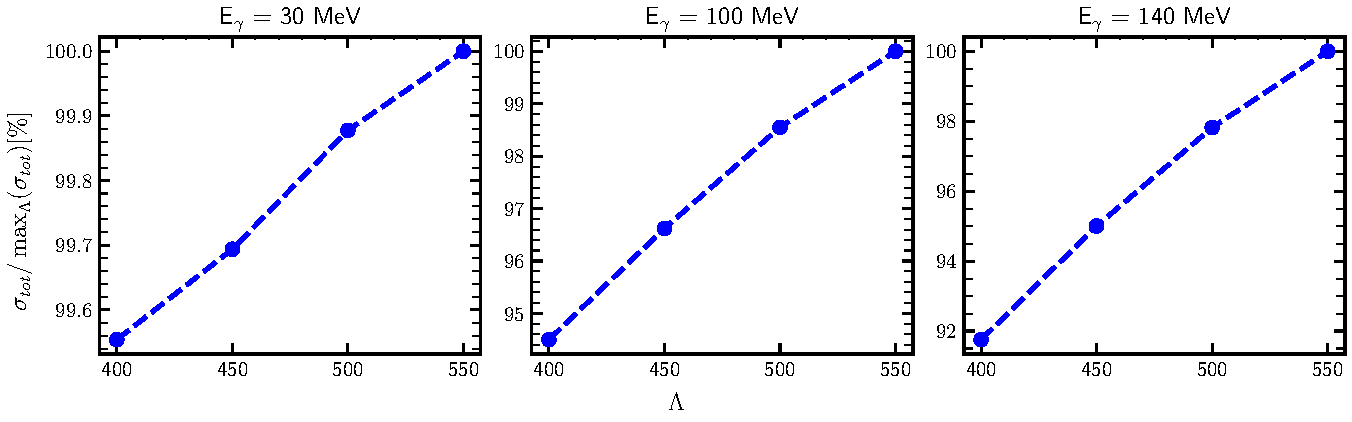
\includegraphics[width=0.95\textwidth]{Figures_De/TOTAL_CROSSSECTION_cutoff.pdf}
        \end{center}
        \caption{Total cross section of the deuteron photodisintegration
        process (normalized to the maximal cross section among all $\Lambda$)
        as a dependance on the cutoff parameter $\Lambda$ 
        for three photon energy E$_\gamma$ values: 30, 100 and 140 MeV.}
        \label{Cutoff_dep}
        \end{figure}

    Another theoretical uncertainty comes from the choice of the cutoff parameter's value 
    of regulator described in the Chapter \ref{sec:intro}.

    In the case of the \gls{sms} interaction its free parameters have been obtained from data for 
    % According to \cite{reinkrebs2018}, where the \gls{sms} potential was presented,
   four values of the cutoff parameter $\Lambda$:
   \SIlist[list-units = single]{400;450;500;550}{\mev} \cite{reinkrebs2018}.
   Using each of these values, one obtains different predictions which, of course, can further differ 
   from actual (experimental) value. Therefore the choice of $\Lambda$ value
   may affect a quality of the prediction.

    To study that I also use the same four values of the $\Lambda$ parameter,
    obtaining in that way set of four predictions each time.
    That is exemplified in \fig{Cutoff_dep}  for the deuteron photodisintegration cross section for the
    photon's energy $E_\gamma = \SIlist{30;100;140}{\mev}$.
    The \gls{sms} model at \gls{n4lo+} with two-nucleon force is used.
    % Comparison of predictions obtained with different values of the 
    % cutoff parameter $\Lambda$ is presented on the Fig.~\ref{Cutoff_dep}.
    Each subfigure shows predictions for the total cross section as 
    a function of the cutoff parameter,
    normalized to the maximum value among all cross sections
    obtained with various $\Lambda$.
    As we can see, for that observable
    there is almost linear dependance with positive linearity coefficient value:
    with higher $\Lambda$ the cross section value increases as well.
    Note that the higher photon's energy is,
    the stronger becomes the cutoff dependance: for $E_\gamma=\SI{30}{\mev}$
    the maximal difference between predictions is around \SI{0.5}{\percent} while
    for \SI{140}{\mev} it increases to more than \SI{8}{\percent}.
    This results are
    generally within our expectations that the chiral model works better at
    smaller energies
    and is therefore less sensitive to the $\Lambda$ value. Let us remind that $\Lambda$ 
    governs the behavior of the potential at small internucleon distances and only higher energy transfer probes that distances. 



    \subsection*{Other theoretical uncertainies}

    There are obviously more sources of theoretical uncertainties. 
    Our model has a number of either intrinsic limitations in precision or 
    some simplifications which may be improved with further developments of the model.
    
    \paragraph{Nuclear currents}
    At the moment, our model is limited to a single nucleon current, which may not be sufficient to accurately describe the processes under consideration.  This limitation will be further discussed and tested in
    Chapter~\ref{chap:results}. To address this issue, we utilize the Siegert theorem, which enables us to
    incorporate some contributions from the two-nucleon current, although it does not yet complete a job.
    It is worth noting
    that the incorporation of the two-nucleon current can significantly affect the predicted observables, as it
    includes additional physical effects that are not accounted for in the single nucleon current. Therefore, the
    ongoing development of a complete chiral two-nucleon current
    is of great importance for our model to improve the accuracy of the predictions.

    \paragraph{Nonrelativistic approach}
    All the results presented here does not include relativistic corrections.
    At the lower energies the relativistic contribution might not be crucial,
    but at the region with higher energy we may see a lack of precision.
    This will be also confirmed and discussed regarding the total cross section
    for the deuteron photodisintegration (see \fig{TOTAL_CROSS}).
    
    \paragraph{Uncertainties in the potential free parameters}
    % Since the chiral potential is of a semi-phenomenological type, the fitting procedure is applied
    % in order to obtain the potential parameters \cite{reinkrebs2018}. 
    % As any fitting, it 
    % introduces an uncertainty to the obtained values which depends on the algorithm's precision.
    % This errors, in principle, are being propagated to the observables as different set of parameters
    % leads to a different predictions.
    % It was extensively investigated how such errors propagate to the observables
    % by choosing different set of potential parameters and comparing obtained 
    % predictions with original values. It had been investigated for the
    % three-nucleon systems \cite{Volkotrub_2020} and resulting uncertainties had been found to be small,
    % especially at higher orders of the chiral \gls{sms} potential (smaller than
    % cutoff and truncation errors). Therefore we neglect thist type of uncertainty in the current thesis.
    % Moreover, estimation of such errors is computationally expensive, since it requires 
    % significant amount of computer processing power (separate calculations for each set of parameters).

    Since the chiral potential is of a semi-phenomenological type, the fitting procedure is applied
    in order to obtain the potential parameters \cite{reinkrebs2018}. 
    The values of the free parameter of the \gls{sms} NN potential as well as free
    parameters of the  3N  interaction  have been  obtained  from the data  by the least square fitting.
    As any fitting procedure, it 
    introduces an uncertainty to the obtained values which depends on the algorithm's precision as
    these values are actually estimators of expectation values only.
    This errors, in principle, are being propagated to the observables as different set of parameters
    leads to a different predictions.
    Indead, in \cite{reinkrebs2018} the whole correlation matrix for free parameters of the  \gls{sms} NN
    force is given. Using that knowledge, it is possible to study the propagation of the uncertainty of NN
    force parameters to 3N observables. It is done in \cite{skibincki_prc_2018,Volkotrub_2020} for the
    elastic and inelastic nucleon-deuteron scattering.
    Resulting uncertainies have been found to be much smaller (typically one order of magnitude)
    than uncertainies arising from truncation errors or cutoff dependance.
    I expect  the same uncertainty level in electromagnetic processes and thus I do not
    intend to study that theoretical error in the presented thesis.
    Moreover, estimation of such errors is computationally expensive, since it requires 
    significant amount of computer processing power (separate calculations for each set of parameters).
    In future it could be interesting to check that type of uncertainty for photodisintegration
    processes but it should be done after completing all pieces of Hamiltonian 
    specifically  after including many-body  electromagnetic currents.

    \paragraph{Uncertainties from the numerical method}
    All my results base on numerical calculations,
    so we can come up with a lot of places were numerical methods with limited 
    precision come into the scene. 
    Our approach is based on the partial wave decomposition 
    and in practice only limited number of partial waves is included 
    (usually for 2N scattering we use all channels up to $j^{max}=4$ which corresponds to 18 partial waves).
    For 3N calculations we use $J^{max}=15/2$\tmp{???} which corresponds to 142 partial waves.
    In addition, I work with some 
    grid of points which is used for the calculation of potential, wave function, numerical integration etc. 
    The choice of grid affect
    a final results' precision. 
    % The same grid is also used for numerical integration
    % (e.g. in \eq{integral2}) where the final integral is also dependant on the points.
    Usually, we use a grid of \tmp{72??} values which was proven to make resulting
    uncertainty small \cite{Glockle1983}.

    \paragraph{Model choice}
    I focus on the \gls{sms} potential, but using another model of interaction 
    in general leads to different predictions. That difference is also a theoretical uncertainty thus
    we use predictions obtained with the semiphenomenological AV18 model in order to compare the chiral results.
    The AV18 model is a widely used and well-established model of nuclear interaction,
    which has been extensively tested and benchmarked against experimental data. By comparing
    the predictions obtained from the SMS potential with those obtained from the AV18 model,
    we can assess the robustness (comparing to  the AV18 results) of our results and determine the extent to which they depend
    on the choice of the interaction model. This comparison also helps to identify the strengths
    and weaknesses of each model and provides insights into the underlying physics of nuclear interactions.

    \paragraph{Machine precision}
    % Finally every computer calculations include limited numerical machine precision which
    % can be noticeable for a complex calculations. We perform our calculation via CPU machine 
    % were particular choice of the processor and memory card may lead to numerical uncertainty.
    % Nevertheless this uncertainty is much smaller then other discussed above. 

    Finally, it should be noted that every computer calculation includes limited numerical machine precision which
    can be noticeable for complex calculations. We perform our calculations via CPU machine, where the particular
    choice of the processor and memory card may lead to numerical uncertainty. However, we have found that this
    uncertainty is much smaller than the uncertainties discussed above, and its impact on our results is
    negligible. We have taken great care to ensure that our calculations are performed using appropriate numerical
    methods and sufficient computational resources to minimize any numerical errors that may arise. 

\chapter{Results}\label{chap:results}

    % In this chapter I will show results of my calculations. I start from the deuteron photodisintegraion process
    % (Section~\ref{sec:de_results}),
    % presenting predictions for the cross section (subsection~\ref{sec:cross_results}) 
    % and polarization observables  (subsection~\ref{sec:polarization_results}).
    % Next, in 
    % Section~\ref{sec:hel_results} I will present my predictions of the observables
    % in $^3$He photodisintegration.
    % In the following Section~\ref{sec:triton_results} the results of calculations for 
    % Triton photodisintegration observables will be lightened. 
    % Finally in Section~\ref{sec:pion_results} I will discuss results of the calculations
    % for the pion absorption from the lowest atomic orbital of $^2$H, $^3$H and $^3$He.

    In this chapter, I will present the results of my calculations. I will begin with the deuteron photodisintegration process in Section~\ref{sec:de_results}, where I will provide predictions for the cross section (Subsection~\ref{sec:cross_results}) and polarization observables (Subsection~\ref{sec:polarization_results}).
    Next, in Section~\ref{sec:hel_results}, I will present my predictions for 
    the observables in $^3$He photodisintegration.
    Moving on to Section~\ref{sec:triton_results}, I will illuminate the results of calculations for
    Triton photodisintegration observables.
    Finally, in Section~\ref{sec:pion_results}, I will discuss the results of the calculations for
    the pion absorption from the lowest atomic orbital of $^2$H, $^3$H, and $^3$He.

\section{Deuteron photodisintegraion}
\label{sec:de_results}
    \subsection{Cross section}
    \label{sec:cross_results}

    In this section I will show the results of my calculation starting from the
    deuteron photodisintegration process. One of the most
    studying observable is obviously the cross section. There is
    a number of papers which present 
    measurement results for both differential and total cross section
    \cite{BOSMAN1979,ARENDS1984,Skopik1974, Moreh1989, Birenbaum1985, Bernabei1986, rachek2007,Ying_Experiment_Deut, DeSanctis_Experiment_Deut} 
    and it is interesting to compare 
    our predictions with that experimental results.

    In \fig{TOTAL_CROSS_small} and \fig{TOTAL_CROSS} 
    I present predictions for the
    total cross section $\sigma_{tot}~[\mu\text{b}]$ which I obtained
    using the chiral \gls{sms} potential at the \gls{n4lo+} order and with 
    the cut-off parameter $\Lambda=\SI{450}{\mev}$.
    From \fig{TOTAL_CROSS_small}, we see that at low photon energies
    (below \SI{50}{\mev})
    both 1NC predictions and results which include 2N contributions
    to the electromagnetic current
    via the Siegert approach, describe experimental results quite well quantitavely.
    We observe that predicions based on the \gls{snc} describe the data 
    only up to approx. \SI{10}{\mev}.
    Beyond that energy
    % We can suppose that the difference with experimental data may come from 
    % the statistical uncertainty of  the data itself, as my predictions
    % are often in between the data from different experiments.
    the \gls{snc} current is clearly not enough
    to describe cross section 
    as corresponding predictions are clearly below the data.
    In that region \gls{snc}+Siegert predictions deliver better data description but 
    overestimate the data.
    % - dashed pink line has much lower values and
    The difference between \gls{snc} and \gls{snc}+Siegert cross section grows with increasing photon energies.
    At \SI{5}{\mev} the difference between \gls{snc} predictions
    and \gls{snc}+Siegert is \SI{297.54}{\micro\barn} (\SI{10.8}{\percent}), increasing energy to 10 MeV
    it is \SI{304.28}{\micro\barn} (\SI{20.4}{\percent})
    and at \SI{20}{\mev} it is \SI{229.50}{\micro\barn} (\SI{39.2}{\percent}).
    % Even with energy increasing from 5~MeV to \SI{20}{\mev} -
    % the difference between predictions has changed from 10.8\% to 39.2\% and
    
    Here and later the relative difference between set of predictions ($x_1$, $x_2$, ..., $x_N$) is calculated
    using the formula:

    \begin{equation}
        \Delta = \frac{\max(x) - \min(x)}{\frac{1}{N}\sum_{i=1}^N x_i} \cdot 100\%,
        \label{eq:relative_diff}
    \end{equation}
    so in the specific case of comparison the date with \gls{snc} current and "\gls{snc} + Siegert" we
    calculate relative difference as 
    $\Delta = \frac{|\sigma^{\gls{snc}+Siegert} - \sigma^{1N}|}{0.5(\sigma^{\gls{snc}+Siegert} + \sigma^{1N})}$.
    
    From \fig{TOTAL_CROSS_small} we see that the gap between these predictions
    continues increasing even more with larger energies.
    This tells us that the Siegert approach works quite well as no additional 2N contributions are taken into account.
    The cross section predictions corrected via Siegert 2N contribution  reproduce 
    experimental data to some extend.
    
    \fig{TOTAL_CROSS_small} reveals the approximated charachter of the Siegert approach.
    It is clear that one has to take with causion Siegert predictions at very small energies.
    Also above \SI{20}{\mev} there is a gap between Siegert results and experimental data,
    which points that more elaborated 2N current should be included in future.
    The observed discrepancy cannot be explained by the cut-off dependance
    (see e.g. \fig{Diff_cross_cutoff} below) or by the low order of chiral potential (see discussion below).

    While my main goal is to describe deuteron photodisintegration
    at energies $\text{E}_\gamma \lesssim \SI{50}{\mev}$, 
    where predictions seem to describe experimental data reasonably well,
    it is also interesting to check how 
    present theory works at higher energies.
    Above $\text{E}_\gamma=\SI{50}{\mev}$
    we can notice that the discrepancy with experimental data is not only 
    quantitative, but also qualitative see \fig{TOTAL_CROSS}.  
    This starts already above $\text{E}_\gamma=\SI{50}{\mev}$ and is especially pronounced at peak around \SI{300}{\mev}
    seen in the experimental data from \cite{Bernabei1986} which is not
    reflected in my predictions. The reason of such discrepancy 
    is most likely coming from the relativistic effects
    which we do not take into account within this work.
    It is also confirmed by the calculations in \cite{ArenhovelPhotodisint1991},
    where authors discuss various NN potentials applied to the deuteron photodisintegration.
    Despite using much simpler models of the nuclear force than those used in this thesis,
    their predictions, which include some relativistic effects, show that such a peak appears in their predictions. 
    
    
    %  The higher energies region is presented in order
    % to investigate how far the predictions are from experimental results and 
    % what should be improved in the future (e.g. include relativistic part). 
    
    \begin{figure}[h]
        \begin{center}
        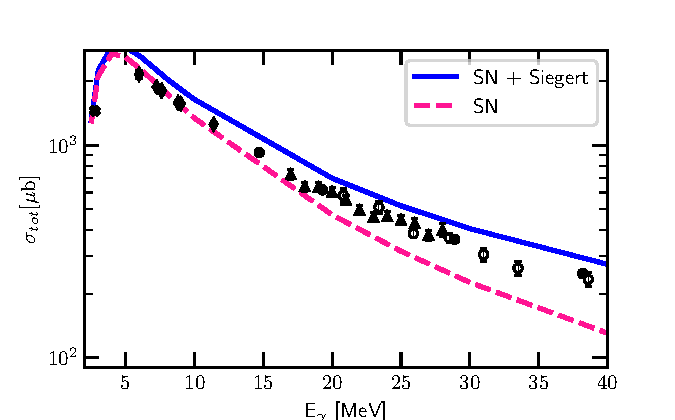
\includegraphics[width=0.75\textwidth]{Figures_De/TOTAL_CROSSSECTION_SMALL_REGION.pdf}
        \end{center}
        \caption{Total cross section $\sigma_{tot}$ for the deuteron photodisintegration process
        as a function of the photon energy E$_\gamma$.
        Solid blue line presents results obtained with \gls{snc}+Siegert 
        and dashed pink line - predictions based on the \gls{snc}.
        In both cases the \gls{sms} \gls{n4lo+} $\Lambda=\SI{450}{\mev}$ force is used.
        The experimental data are from \cite{Bernabei1986} (black filled circles),
        \cite{BOSMAN1979} (empty circles),
        % \cite{ARENDS1984} (squares),
        \cite{Skopik1974} (triangles),
        \cite{Moreh1989} (bold cross "X") and
        \cite{Birenbaum1985} (diamonds).
        }
        \label{TOTAL_CROSS_small}
    \end{figure}

    
    \begin{figure}[htb!]
        \begin{center}
        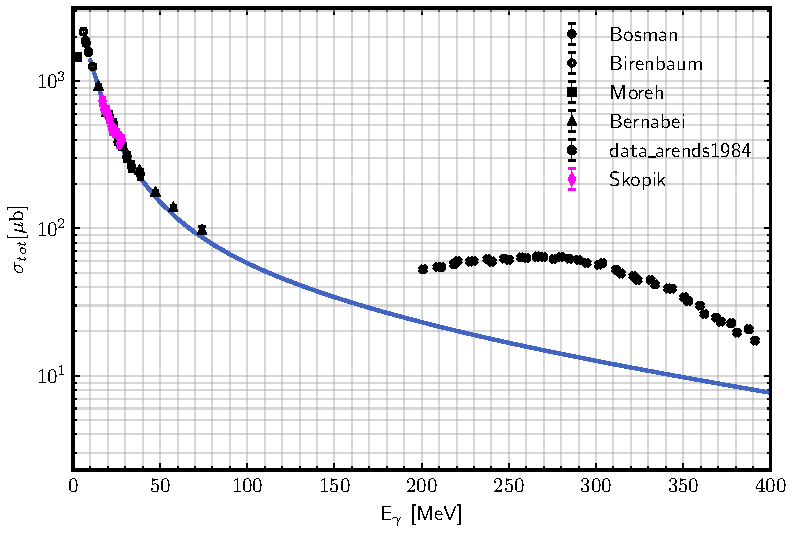
\includegraphics[width=0.75\textwidth]{Figures_De/TOTAL_CROSSSECTION.pdf}
        \end{center}
        \caption{The same as in \fig{TOTAL_CROSS_small} but for the energy range 2.5 - 400 MeV.
        The experimental data are the same as in \fig{TOTAL_CROSS_small}
        but supplemented by the data above $\text{E}_\gamma=\SI{200}{\mev}$ from
        \cite{ARENDS1984} (crosses).
        }
        \label{TOTAL_CROSS}
    \end{figure}

    \begin{figure}[htb!]
        \begin{center}
            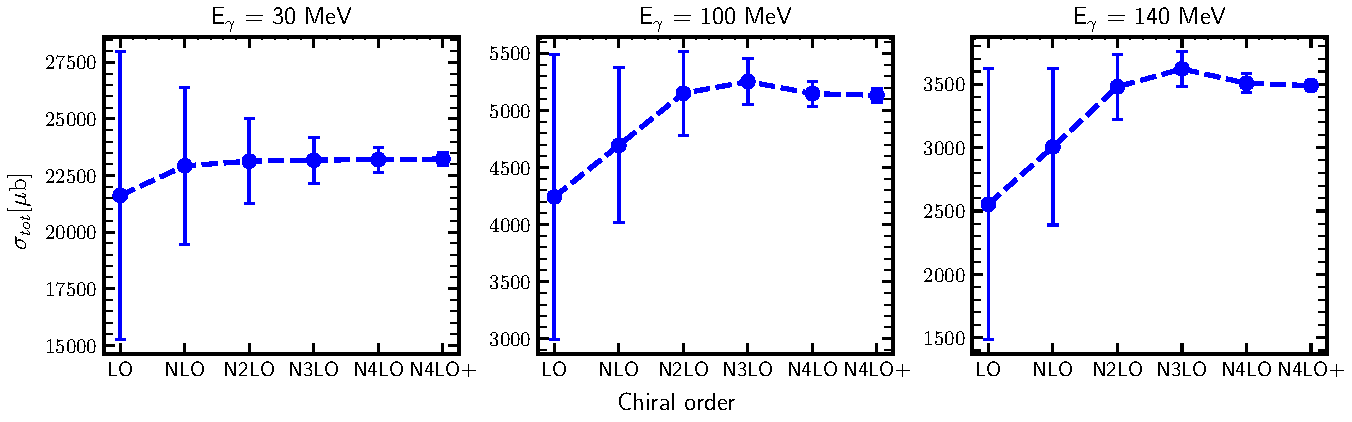
\includegraphics[width=0.95\textwidth]{Figures_De/TOTAL_CROSSSECTION_Truncation.pdf}
        \end{center}
        \caption{Total cross section of the deuteron photonisintegration
        process as a dependence on the chiral order for three photon energy E$_\gamma$ values: \SIlist[list-units = single]{30;100;140}{\mev}.
        Error bands show an estimated truncation error at each order.}
        \label{Trunc_100}
    \end{figure}
    
    In Fig. \ref{Trunc_100} I present the
    total cross-section for the deuteron photodisintegration 
    at three photon energy values: \SIlist[list-units = single]{30;100;140}{\mev} as a function of the chiral order.
    Error bars show truncation errors calculated using Eq.~\ref{trunc2}~-~\ref{trunc5}.
    One can see that the truncation errors are being reduced with each consecutive chiral order. 
    At \gls{lo} uncertainty is the biggest: \SI{29.46}{\percent} at $\text{E}_\gamma = \SI{30}{\mev}$,
    \SI{29.46}{\percent} at $\text{E}_\gamma = \SI{100}{\mev}$ and
    \SI{41.82}{\percent} at $\text{E}_\gamma = \SI{140}{\mev}$.
    At \gls{n4lo+} it is hardly visible at presented scale and amounts up to 
    \SI{1.3}{\percent} for each energy(however decreasing with the chiral order).
    For each energy the prediction is within the uncertainty range at lower orders.
    We see that at lower energy $\sigma_{tot}$ already at NLO reaches valve which remains
    practically unchanged at higher orders.
    Contrary, at two higher energies, contributions from higher orders are necessary to obtain 
    stable predictions up to approx. \gls{n3lo}.

        
    Figures \ref{Diff_cross_order_pw} and \ref{Diff_cross_err} show my predictions 
    for the differential cross section
    $\frac{d\sigma}{d\Omega}$.
    In both figures the top, middle and bottom row shows predictions at 
    $\text{E}_\gamma = \SIlist[list-units = single]{30;100;140}{\mev}$, respectively.
    For all predictions, the contributions of the 2N current are taken into account via the Siegert theorem,
    and unless stated otherwise, I utilize the \gls{sms} \gls{n4lo+} potential.
    % They all are organized in a similar way: the left panel
    % presents predictions obtained using \gls*{sms} potential at different chiral orders (from LO to \gls{n4lo+})
    % with cut-off parameter $L = \SI{450}{\mev}$,
    % the middle panel includes the truncation error's bands (described in Sec. \ref{sec:deu\text{T}_bound})
    % for each chiral order starting
    % from NLO. And the right panel shows predictions obtained with different values of the
    % cut-off parameter at the chiral order \gls{n4lo+}.
    The left column of \fig{Diff_cross_order_pw} shows the predictions obtained at 
    different chiral orders (from LO to \gls{n4lo+}) and with $\Lambda=\SI{450}{\mev}$.
    Looking at the best predictions (\gls{n4lo+}, $\Lambda=$~\SI{450}{\mev}) for each
    energy, I
    conclude that the higher photon energy is, the larger 
    difference between the theoretical predictions and experimental 
    data is. At $\text{E}_\gamma = \SI{30}{\mev}$ (top panel) my predictions
    almost perfectly match the data and the difference is almost always
    within the tripled experimental uncertainties. 
    Moving to  $\text{E}_\gamma=\SI{100}{\mev}$ (middle row)
    the description of the data is deteriorating: theoretical
    predictions still match the data qualitatively, but
    the gap for proton emission angle $\theta_p$ in range ($\ang{60} < \theta_p < \ang{130}$) 
    is up to \SI{32}{\percent} (of the predicted value)
    and relative difference (calculated with \eq{eq:relative_diff}) is up to
    \SI{7}{\percent}.
    At the highest energy (bottom row), it is even hard to say about 
    good qualitative description: the general trend of the
    angular dependence is presented, but the predictions are 
    far from the experimental points.
    The relative difference between experimental data and predictions obtained with $N^4LO+$ and $\Lambda=$~\SI{450}{\mev} at \SI{30}{\mev} is less then \SI{13}{\percent}
    and absulute difference is < \SI{3.07}{\micro \barn \per \steradian}.
    At \SI{100}{\mev} descripancy is larger and relative difference reaches 46\% with absolute difference up to \SI{1.39}{\micro \barn \per \steradian}.
    Coming to \SI{140}{\mev} the relative difference 
    increases up to \SI{48.6}{\percent} and absolute - \SI{1.93}{\micro \barn \per \steradian}.
    What may be helpful
    for a better data description is a 2N current 
    and relativistic correction, mentioned earlier.
    We observe improvements introduced by each subsequent chiral order, but 
    stabilization shows that some ingredients beyond 2N potential are missing.

    Obtained results at each energy confirm the convergence 
    of the predictions with respect to the chiral order.
    We see that the cross section at LO is far from both experimental 
    data and the most advanced \gls{n4lo+} predictions, and
    the higher photon energy, the larger this
    difference is. With each subsequent chiral order, the 
    curves are more closer to each other and the difference
    between \gls{n4lo} and \gls{n4lo+} is hardly visible at scale used in \fig{Trunc_100}.
    The relative difference between these two predictions at $\text{E}_\gamma=\SI{30}{\mev}$ around the point of maximum 
    ($\theta_p = \ang{80}$) is \SI{0.05}{\percent} which is \SI{0.02}{\micro \barn \per \steradian};
    at \SI{100}{\mev} and $\theta_p = \ang{107}$ it is \SI{0.79}{\percent} (\SI{0.025}{\micro \barn \per \steradian});
    and at \SI{140}{\mev} (same angle) it is \SI{1.8}{\percent} (\SI{0.043}{\micro \barn \per \steradian}).
    Having such a small differences between predictions from two highest chiral orders,
    I can conclude that predictions are converged and 
    using NN potential beyond \gls{n4lo+} chiral orders would rather not bring significant contribution 
    to the cross section values. 
    The difference with experimental data is systematic 
    and is not related with the chiral order. 
    

    Predictions obtained with the \gls{av18} potential 
    (dashed-dotted purple line in the \fig{Diff_cross_order_pw} left)
    are very similar to these from the \gls{n4lo+} \gls{sms} force at lower energies
    (relative difference at $\text{E}_\gamma=\SI{30}{\mev}$ is \SI{0.06}{\percent}
    at the point of maximum $\theta_p = \ang{80}$) and with increasing energy to \SI{140}{\mev}
    it growes up to \SI{3.1}{\percent} at the same scattering angle. 
    It can be connected with our potential's quality loss, but \gls{av18} can
    be struggling with high energies as well.
    That once again shows that other 
    components of Hamiltonian become important at that energies.

    
    In the right column of the \fig{Diff_cross_order_pw} I compare predictions
    based on various assumptions on nuclear current and dynamical mechanism.
    I again use \gls{sms} \gls{n4lo+}, $\Lambda=\SI{450}{\mev}$ force.
    At the lowest energy predictions comprising the plane-wave component only (without rescattering part)
    and taking currents as SNC+Siegert, show relatively small deviation from the full predictions, but the difference increases at larger energies.
    With $\text{E}_\gamma=\SI{30}{\mev}$ the relative difference is \SI{10}{\percent} (\SI{4.03}{\micro \barn \per \steradian})
    at $\theta_p = \ang{80}$. Difference at \SI{100}{\mev} and the same angle is \SI{4}{\percent} (\SI{0.21}{\micro \barn \per \steradian})
    and at \SI{140}{\mev} it is \SI{7}{\percent} (\SI{0.21}{\micro \barn \per \steradian}).
    In contrast, predictions without two-body current component (1NC) have much larger gap with full prediction:
    the difference is \SI{46.5}{\percent} (\SI{13.67}{\micro \barn \per \steradian}) at \SI{30}{\mev},
    \SI{78.6}{\percent} (\SI{2.88}{\micro \barn \per \steradian}) at \SI{100}{\mev} and
    \SI{77.8}{\percent} (\SI{1.68}{\micro \barn \per \steradian}) at \SI{140}{\mev}
    at the same $\theta_p=\ang{80}$.
    Obviously 2NC contributions are extremely important in this case, the difference connected with them
    is much bigger then theoretical uncertainties or even rescattering contribution.
    For other scattering angles, especially $\theta_p=\ang{0}$ or $\theta_p=\ang{180}$,
    the role of two-body current or FSI is relatively even more pronounced.


    The \fig{Diff_cross_err} (left)
    presents theoretical truncation uncertainties.
    That confirms our expectations
    that for the regarded photo reaction chiral order
    \gls{n4lo+} is able to produce converged predictions: 
    the black band (representing truncation error at \gls{n4lo+}) is hardly visible
    for the $\text{E}_\gamma=$~\SI{30}{\mev}
    (the relative error for \gls{n4lo+} at \ang{80} is only \SI{0.12}{\percent})
    and is also quite narrow for larger energies (at \SI{140}{\mev} 
    the error at the same angle is \SI{1.46}{\percent}).
    At the lower chiral orders, this band is obviously much wider:
    at \gls{n2lo} it is \SI{1.25}{\percent} at $\text{E}_\gamma=$~\SI{30}{\mev}
    and \SI{15.0}{\percent} at $\text{E}_\gamma=$~\SI{140}{\mev}.
    I note, that the magnitude of the truncation error
    only very tiny depends on the scattering angle.
    
    Last but not least, in the right column of \fig{Diff_cross_err}
    I show the cut-off dependence of the differential cross section.
    In the ideal case that dependence is so weak that
    the choice of the parameter $\Lambda$ would not introduce significant 
    changes. In practice the choice of this parameter is 
    important as it makes a noticeable variation in prediction at higher energies.
    Namely, while at $\text{E}_\gamma=$~\SI{30}{\mev} the cut-off dependence is so tiny
    that, in fact, all the lines (for different $\Lambda$ values)
    overlap each other and we cannot distinguish them with the naked eye:
    the relative difference at the maximum of the cross section is \SI{0.08}{\percent}.
    This is approximately $\frac{2}{3}$ smaller than truncation error discussed above.
    However, with increasing photon energy up to \SIlist{100; 140}{\mev} 
    (middle and bottom rows of the right column of \fig{Diff_cross_err}) the spread becomes bigger:
    the  uncertainty related to the 
    $\Lambda$-dependence is  \SI{3.35}{\percent} at \SI{100}{\mev}
    and \SI{5.66}{\percent} at \SI{140}{\mev} (the same $\theta_p$).
    Thus at two higher energies the cut-off dependence becomes more important
    than truncation errors.
    That shows, that proper choice of the $\Lambda$ is important.
    However, if I restrict myself to $\Lambda=\SIlist{450;500}{\mev}$,
    the dependence drops to \SI{1.98}{\percent} at $\text{E}_\gamma=\SI{140}{\mev}$.
    Such a restriction is advocated by better description of the scattering data
    delivered by the SMS potential for that two values of $\Lambda$.

    In the \fig{Cutoff_dep} we have already seen that the total
    cross section for the same energies has the cut-off spread
    around \SI{4.5}{\percent} for \SI{100}{\mev} and \SI{8}{\percent} for \SI{140}{\mev}
     For $\text{E}_\gamma=\SI{30}{\mev}$ it is below  \SI{1}{\percent}.
     It means that even cut-off dependance for that total cross section (affected
     by the extreme values close to $\theta_p = 0$ or $\theta_p = 180$)  are
     relatively small, especially at the lower energies.


    \begin{figure}[h]
        \centering
        \begin{subfigure}[t]{0.46\textwidth}
            \caption{}
            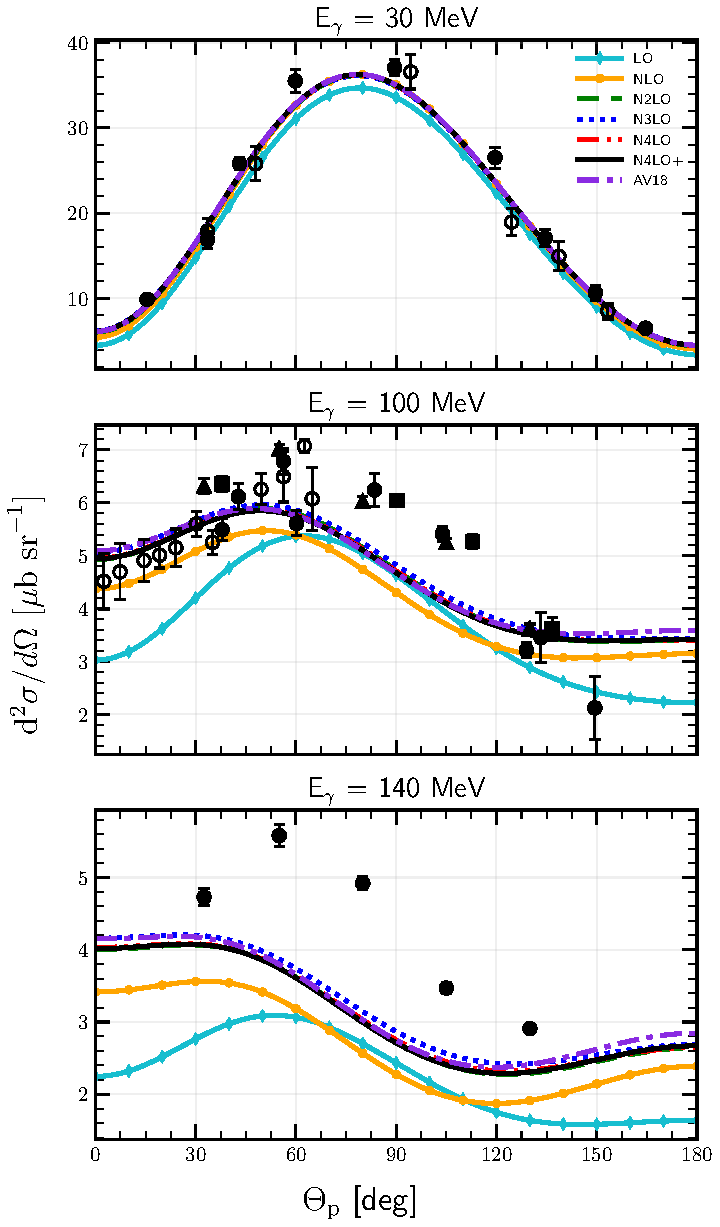
\includegraphics[width=\textwidth]{Figures_De/CROSS2_order_vert.pdf}
            \label{Diff_cross_order}
        \end{subfigure}
        \begin{subfigure}[t]{0.46\textwidth}
            \caption{}
            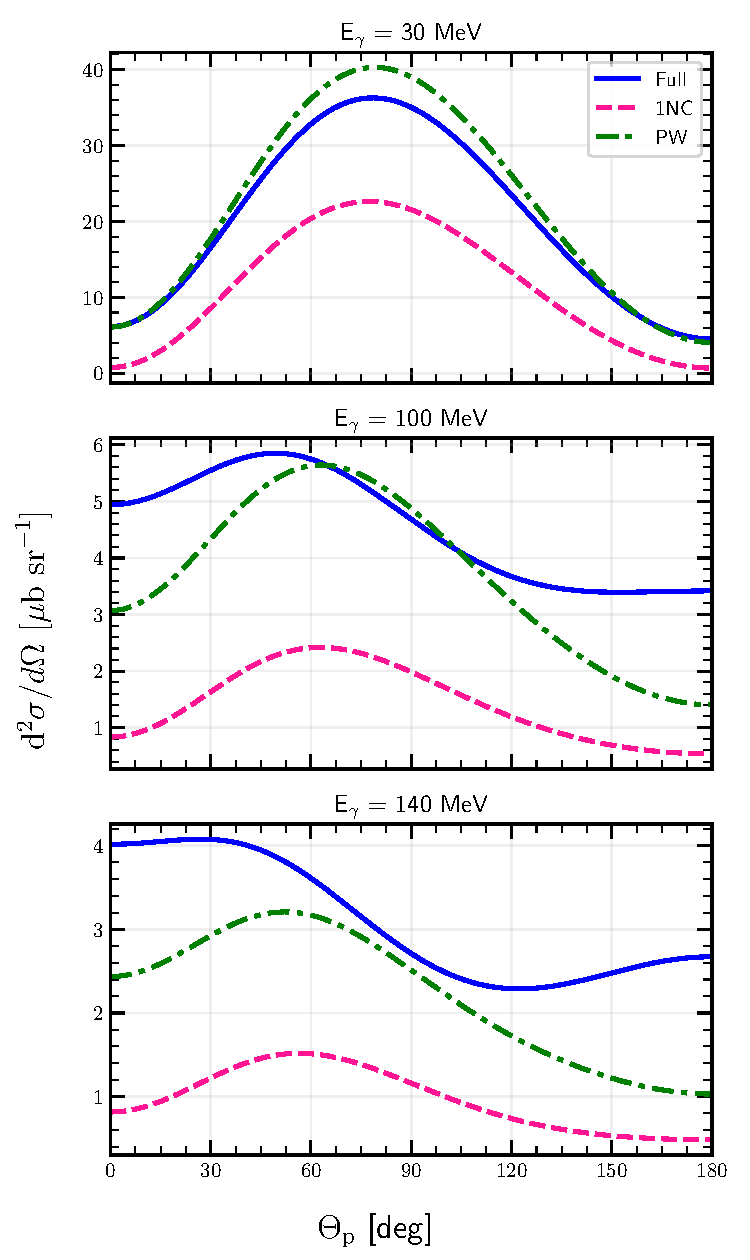
\includegraphics[width=\textwidth]{Figures_De/Diff_cross_pw_1nc.pdf}
            \label{Diff_cross_pw_1nc}
        \end{subfigure}
        \caption{Differential cross section $\frac{d^2\sigma}{d\Omega}$
        as a function of the outgoing proton momentum polar angle $\theta_p$ in the center of mass frame 
        for the photon energy \SI{30}{\mev} (top), \SI{100}{\mev} (middle) and \SI{140}{\mev} (bottom).
        {\bf (a)} Results obtained using the \gls{sms} potential
        at different chiral orders (from LO to \gls{n4lo+}) with the cut-off parameter $\Lambda=\SI{450}{\mev}$ and 
        2NC contributions taking via the Siegert theorem.
        For the sake of comparison, predictions obtained with the \gls*{av18} potential are shown
        by dashed-dotted purple line.
        Data points (filled and empty circles) are from \cite{Ying_Experiment_Deut}
        for $\text{E}_\gamma=\SIlist[list-units = single]{30; 100}{\mev}$
        and from \cite{DeSanctis_Experiment_Deut} for $\text{E}_\gamma=\SI{140}{\mev}$.
        {\bf (b)} Predictions obtained with the chiral \gls{n4lo+} potential and $\Lambda=\SI{450}{\mev}$
        with various models of nuclear current and scattering state.
        The blue solid curve represents our most complete predictions
        comprising the plane-wave plus rescattering parts and \gls{snc}+Siegert current propagator 
        (the same as \gls{n4lo+} line in (a)).
        The pink dashed curve shows predictions obtained with
        the single-nucleon current only (without applying the Siegert theorem) and the green dashed-dotted
        curve represents predictions with the full current (\gls{snc} + Siegert) but plane-wave part only.
        }
        % Results in {\bf (a)} are obtained using \gls*{sms} potential
        % at different chiral orders (from LO to \gls{n4lo+}) with the cut-off parameter $\Lambda=\SI{450}{\mev}$ and 
        % 2NC contributions taking via Siegert theorem.
        % Data points (filled and empty circles) are from \cite{Ying_Experiment_Deut}
        % for (\SIlist[list-units = single]{30; 100}{\mev})
        % and \cite{DeSanctis_Experiment_Deut} (for energy \SI{140}{\mev}).
        % Predictions obtained with chiral \gls{n4lo+} potential and $\Lambda=\SI{450}{\mev}$ are on {\bf (b)}.
        % Blue solid line is a best predictions we have (plane-wave plus rescattering parts, 1NC + Siegert), pink dashed line shows predictions obtained with
        % single-nucleon current only (without Siegert contributions) and green dashed-dotted line
        % is a prediction with plane-wave part only - without rescattering.}
        \label{Diff_cross_order_pw}
    \end{figure}


        
    \begin{figure}[h]
        \centering
        \begin{subfigure}[t]{0.46\textwidth}
            \caption{Truncation error bands.}
            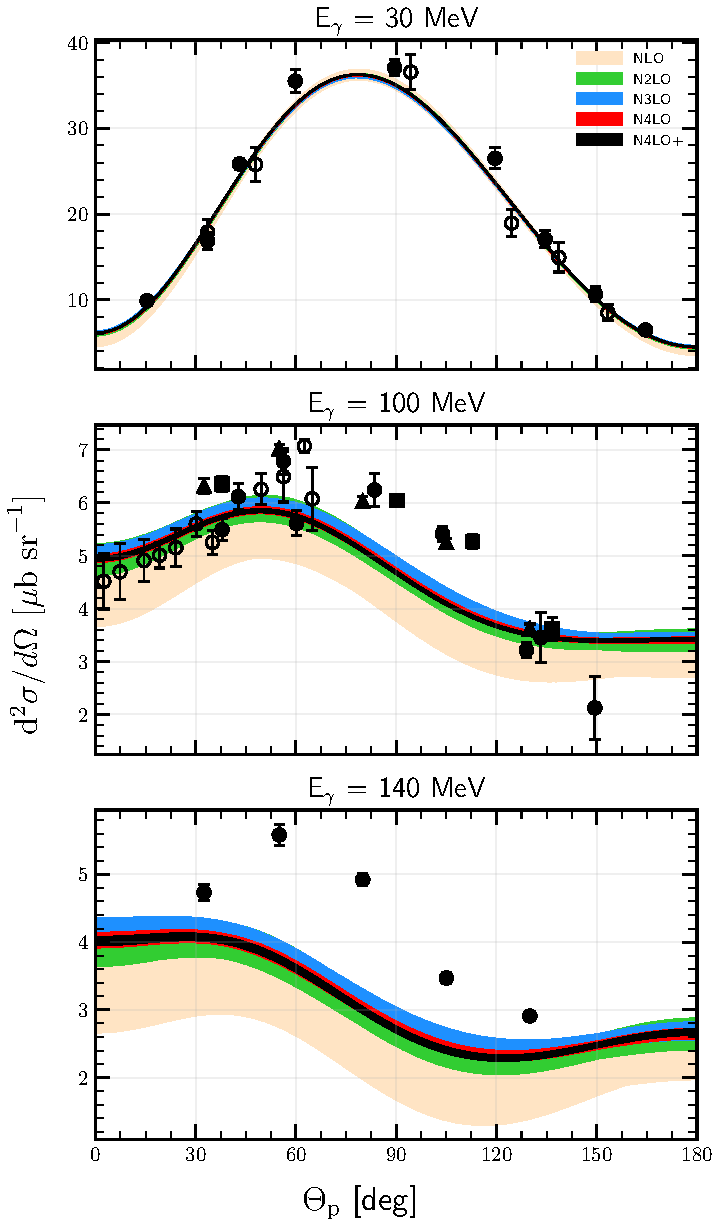
\includegraphics[width=\textwidth]{Figures_De/CROSS2_truncation_vert.pdf}
            \label{Diff_cross_truncation}
        \end{subfigure}
        \begin{subfigure}[t]{0.46\textwidth}
            \caption{Cutoff dependence.}
            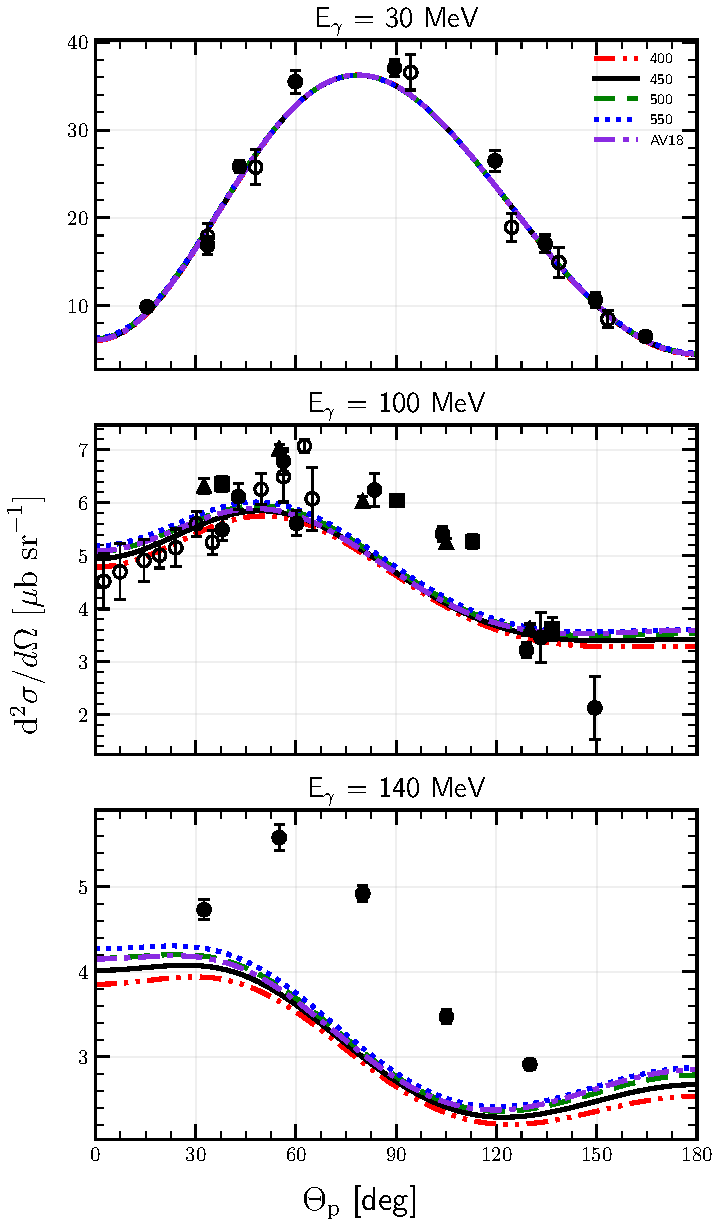
\includegraphics[width=\textwidth]{Figures_De/CROSS2_cutoff_vert.pdf}
            \label{Diff_cross_cutoff}
        \end{subfigure}
        \caption{Theoretical uncertainies 
        for the differential cross section $\frac{d^2\sigma}{d\Omega}$
        as a function of the outgoing proton's momentum polar angle $\theta_p$ in the center of mass frame 
        for the photon energy is \SI{30}{\mev} (top row), \SI{100}{\mev} (middle row) and \SI{140}{\mev} (bottom row).
        {\bf(a)} The truncation error bands obtained using the \gls{sms} potential
        at different chiral orders (from NLO to \gls{n4lo+}) 
        with the cut-off parameter $\Lambda=\SI{450}{\mev}$ and 2NC contributions taking via the Siegert approach.
        {\bf (b)} Results obtained using different values of the cut-off parameter $\Lambda$.
        The double-dotted-dashed red curve, the solid black line, the dashed green line
        and the dotted blue line represent predictions obtained 
        with $\Lambda=\SIlist[list-units = single]{400;450;500;550}{\mev}$ respectively
        and the chiral potential \gls{n4lo+}. 
        Data points are the same as in \fig{Diff_cross_order}}
        \label{Diff_cross_err}
    \end{figure}

    \clearpage

    \subsection{Polarization observables}
    \label{sec:polarization_results}

    In this subsection I will present my predictions for the 
    selected polarization observables in the deuteron photodisintegration process
    at two photon energies: $\text{E}_\gamma = \SI{30}{\mev}$ and
    $\text{E}_\gamma = \SI{100}{\mev}$.
    A priori, various polarization states and measurements
    are thinkable for the $\gamma + \text{d}$ scattering.
    Polarization of the target deuteron leads to the deuteron
    analyzing power.
    Similarly using the polarized photons result in the photon asymmetry measurements.
    Using both polarized photon and deuteron allows for spin
    correlation measurement.
    Finely, detecting spin polarization of at least one nucleon in the final state would deliver
    final polarization or spin transfer coefficients. 
    However, such experiments are very challenging and, up to my best knowledge,
    have not been done yet at regarded here photon energies.
    Thus, in the following I will restrict myself to results for polarization
    observables arising from the polarization of the initial particles.

    I start with deuteron vector $i\text{T}_{11}$ and tensor $\text{T}_{20}$, $\text{T}_{21}$ and $\text{T}_{22}$
    analyzing power, which arise from various spin state of the deuteron.
    
    Deuteron tensor analyzing powers can be calculated via cross section as it is defined in \cite{rachek2007}:
    
    \begin{eqnarray}
        % \begin{aligned}
            \frac{d \sigma}{d \Omega}= \frac{d \sigma_0}{d \Omega}\left\{1-\sqrt{3 / 4} P_z \sin \theta_H \sin \phi_H T_{11}\right.
            +\sqrt{1 / 2} P_{z z}\left[\left(3 / 2 \cos ^2 \theta_H-1 / 2\right) T_{20}\right. - \nonumber \\
            -\sqrt{3 / 8} \sin 2 \theta_H \cos \phi_H T_{21} 
            \left.\left.+\sqrt{3 / 8} \sin ^2 \theta_H \cos 2 \phi_H T_{22}\right]\right\},
        % \end{aligned}
    \end{eqnarray}
    where $\sigma_0$ is the unpolarized cross section, $P_z$ ($P_{zz}$)
    the vector (tensor) target polarization, $\theta_H$ - the angle
    between polarization axis and photon momentum,
    and $\phi_H$ - is the angle between the polarization plane 
    (containing the polarization axis and momentum of the photon),
    and the reaction plane (containing momenta of the proton
    and neutron).

    In the Figures \ref{T20_T21_30} (a, b) and \ref{T22_T11_30}(a,b)
    I show my predictions at $\text{E}_\gamma = \SI{30}{\mev}$, for the
    $\text{T}_{20}$, $\text{T}_{21}$, $\text{T}_{22}$  and $i\text{T}_{11}$ respectively as functions 
    of the outgoing proton momentum polar angle $\theta_p$ in the \gls{cm} frame. Each of them
    is organized in the similar way: the top
    panel shows a dependence of the predictions on the 
    chiral order of the potential. The middle subfigure is
    showing a correspondent truncation error for each of the 
    predictions from a top row (except LO, because its uncertainty is
    too large and will spoil clarity of the figure). The last (bottom)
    panel shows the cut-off dependence at the chiral
    order \gls{n4lo+}. 
    All results have been obtained using \gls{snc}+Siegert model of nuclear current.

    All the analyzing powers presented here show excellent convergence 
    upon a chiral order as it is hard to distinguish the predictions
    from each subsequent order starting from the \gls{n2lo}.
    The relative width of the \gls{n4lo+} truncation band 
    for T$_{20}$, T$_{21}$ and T$_{22}$
    are \SIlist{0.06; 0.05; 0.19}{\percent}, respectively (at $\theta_p=$ \ang{90}, \ang{60} and \ang{90}, respectively).
    The slowest convergence is observed for $i\text{T}_{11}$ (\fig{T11_30_vert})
    where we can recognize \gls{n2lo} band in the figure.
    Nevertheless, at the \gls{n4lo+}
    the width truncation band at $\theta_p = \ang{20}$ (maximum point)
    is only a \SI{0.2}{\percent}.
    The cut-off dependence for all regarded observables is weak and 
    predictions for each value of the $\Lambda$ are hardly separable 
    with the naked eye.
    The relative spread of the predictions based on various $\Lambda$ at the same angles as above 
    are \SIlist{0.87; 0.94; 3.42; 0.68}{\percent} for T$_{20}$, T$_{21}$, T$_{22}$ and $i\text{T}_{11}$, respectively.


    Corresponding predictions at the photon energy $\text{E}_\gamma = \SI{100}{\mev}$
    (Figs. \ref{T20_T21_100} and \ref{T22_T11_100}) preserve similar
    trends for each observable. 
    In general, predictions are being converged starting
    even from the \gls{n2lo} and only for the $i\text{T}_{11}$
    I find
    that truncation error's bands are noticeably wide
    even at \gls{n4lo} and \gls{n4lo+}.
    Cutoff dependence at this energy is a bit stronger
    compared to those at $\text{E}_\gamma = \SI{30}{\mev}$, especially
    for 
    $\text{T}_{22}$ and $i\text{T}_{11}$ analyzing powers (\fig{T22_T11_100} vs \fig{T22_T11_30}),
    where one can see 
    slightly stronger discrepancy at the maxima and minima points.
    
    The choice of $\Lambda$ does not affect predictions substantially
    even at that higher energy:
    the relative spread among all cut-offs for T$_{20}$ is \SI{1.54}{\percent}
    around the point of maximum ($\theta_p = \ang{90}$).
    For other components of the tensor analyzing power spread amounts up to:
    \SI{0.14}{\percent} at $\theta_p = \ang{60}$ for T$_{21}$;
    \SI{3.68}{\percent} at $\theta_p = \ang{90}$ for T$_{22}$;
    and \SI{4.91}{\percent} at $\theta_p = \ang{75}$ for $i\text{T}_{11}$.
    We see again that $i\text{T}_{11}$ has much larger spread in the maximum and
    is more sensitive to the cut-off choice.
    However, summarising my findings 
    for the deuteron tensor analyzing powers,
    I conclude that cut-off dependence is generally weak
    also at $\text{E}_\gamma = \SI{100}{\mev}$.

    Turning our attraction to the chiral order convergence, we
    observe that predictions are mostly converged starting either from \gls{n2lo} or \gls{n3lo}.
    The relative width of \gls{n4lo+} truncation band 
    for T$_{20}$, T$_{21}$ and T$_{22}$
    are \SIlist{0.7; 0.7; 0.04}{\percent} respectively (at the same angles as used above).
    Another case is $i\text{T}_{11}$, for which this width is much larger: \SI{6.8}{\percent} at $\theta_p = \ang{20}$.
    The truncation uncertainty for all analyzing powers is much lower than one,
    related to the choice of the cut-off parameter.
    Although, $i\text{T}_{11}$ seems to be more sensitive both
    to the choice of the cut-off parameter and to the chiral order than other regarded observables.
    Even for $i\text{T}_{11}$, cut-off spread is almost twice larger than truncation error.
    Standing out of other tensor components, $i\text{T}_{11}$ can be useful for the investigation of 
    the cut-off dependence of the model.
    Of course, we can repeat once more that 
    our model is less accurate at higher energies which is reflected
    in a stronger cut-off dependence and slower chiral convergence.
    However, I conclude that even at these energies tensor analyzing powers are
    well converged with respect to the chiral order.

    Comparison of the predictions obtained using the chiral \gls{n4lo+} potential
    $\Lambda = \SI{450}{\mev}$ with ones obtained taking \gls{av18} potential
    show a very good agreement: the relative difference at $\text{E}_\gamma=\SI{30}{\mev}$
    is below \SI{6}{\percent} for the regarded tensor analyzing powers at specified angles.
    Picture at  $\text{E}_\gamma=\SI{100}{\mev}$ is even better: the difference does not exceed 
    \SI{4}{\percent} for all observables and whole range of scattering angles.


    \begin{figure}[htb]
        \centering
        \begin{subfigure}[b]{0.46\textwidth}
            \caption{T$_{20}$}
            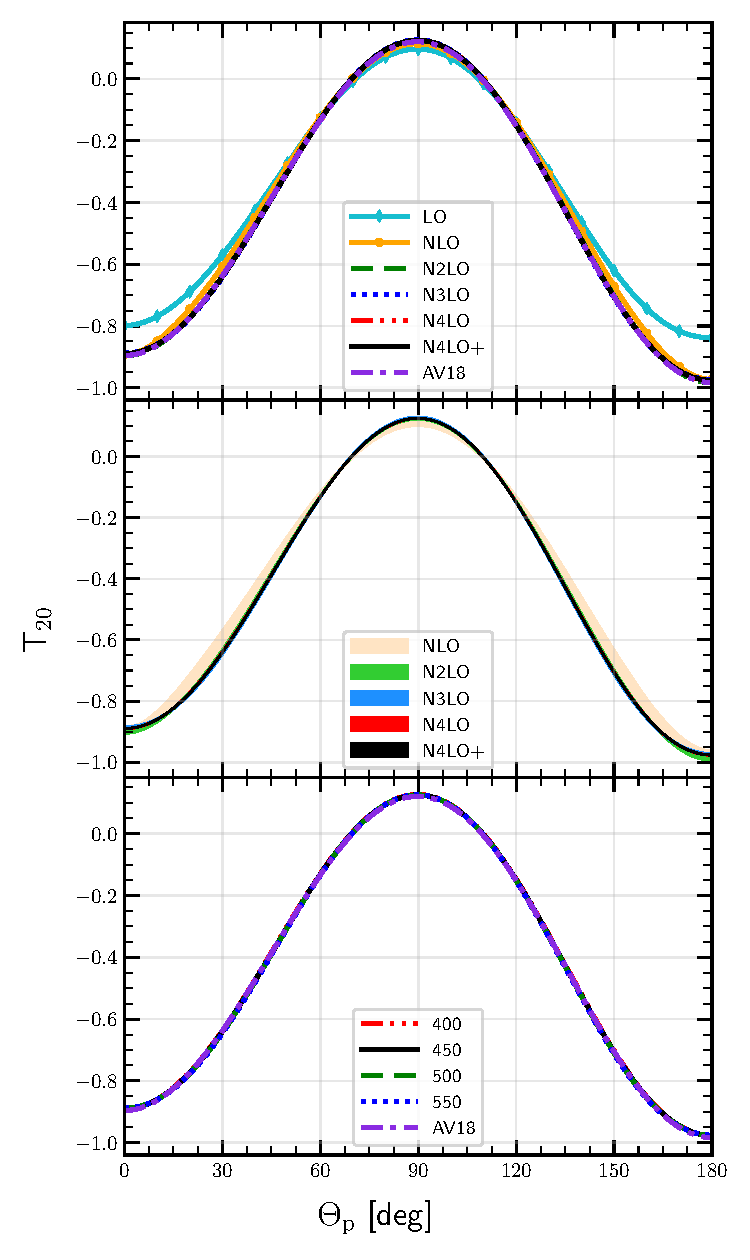
\includegraphics[width=\textwidth]{Figures_De/T20D2_30mev.pdf}
            \label{T20_30_vert}
        \end{subfigure}
        \begin{subfigure}[b]{0.46\textwidth}
            \caption{T$_{21}$}
            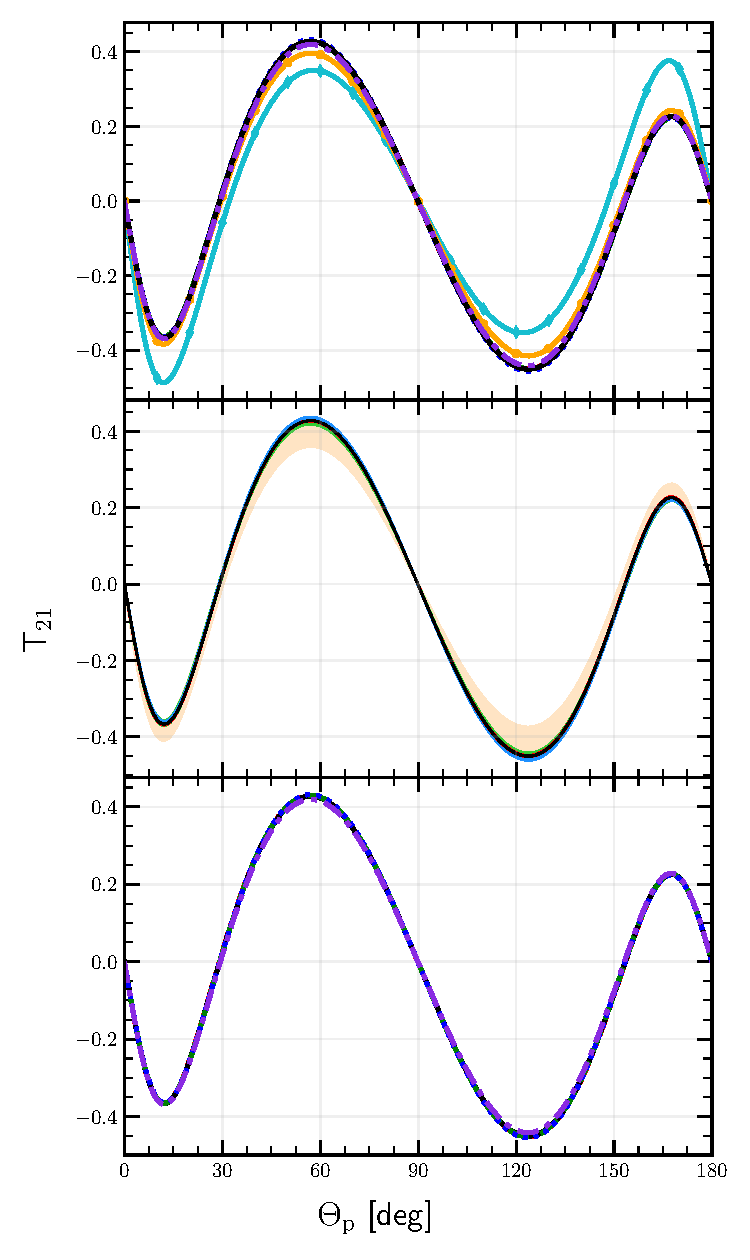
\includegraphics[width=\textwidth]{Figures_De/T21D2_30mev.pdf}
            \label{T21_30_vert}
        \end{subfigure}
        \caption{The deuteron tensor analyzing powers T$_{20}$  {\bf (a)}
        and T$_{21}$ {\bf (b)}
        as a function of the outgoing proton angle $\theta_p$ in the \glsxtrlong{cm} frame 
        for the photon energy $\text{E}_\gamma = \SI{30}{\mev}$.
        Top row presents results obtained using the \gls{sms} potential
        at different chiral orders (from LO to \gls{n4lo+}) with the cut-off parameter $\Lambda=\SI{450}{\mev}$.
        The middle row shows truncation errors for each 
        chiral order starting from NLO and
        the bottom row presents a cut-off dependence at \gls{n4lo+}.
        For the sake of comparison, predictions obtained with the \gls{av18} potential are given as well.
        For all predictions \gls{snc}+Siegert model is used.}
        \label{T20_T21_30}
    \end{figure}

    \begin{figure}[htb]
        \centering
        \begin{subfigure}[b]{0.46\textwidth}
            \caption{T$_{22}$}
            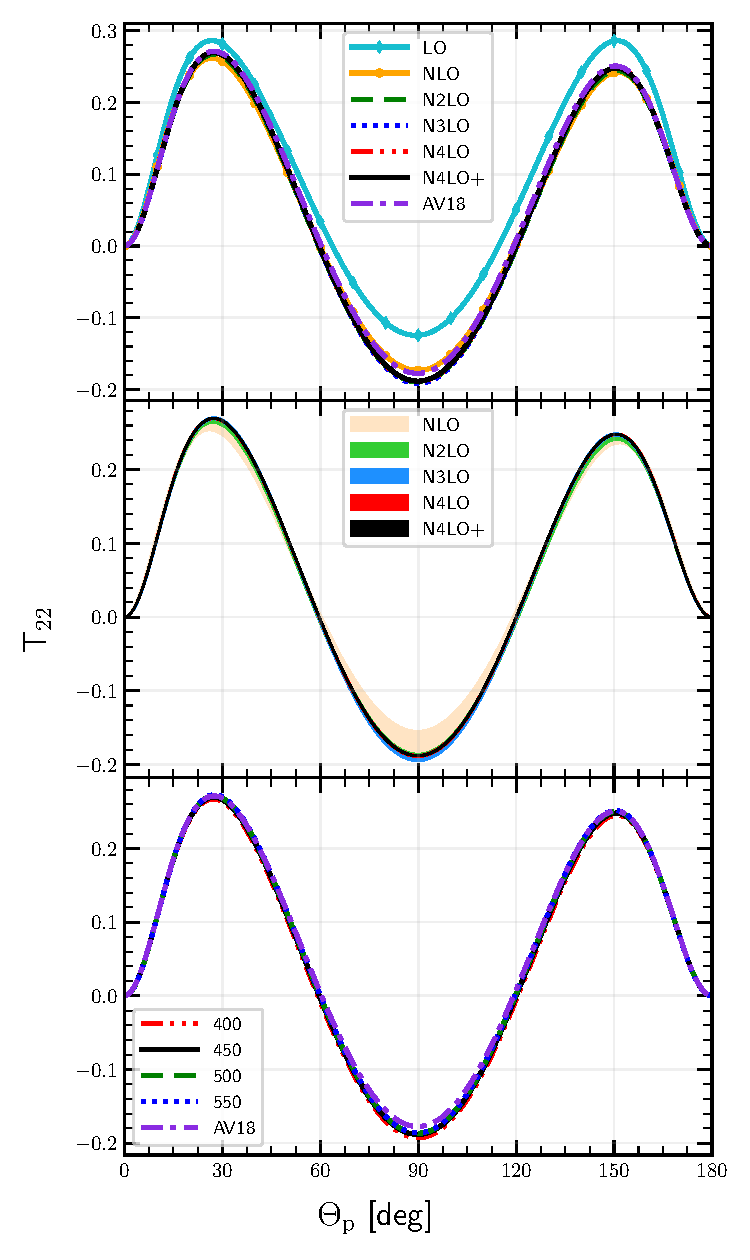
\includegraphics[width=\textwidth]{Figures_De/T22D2_30mev.pdf}
            \label{T22_30_vert}
        \end{subfigure}
        \begin{subfigure}[b]{0.46\textwidth}
            \caption{$i\text{T}_{11}$}
            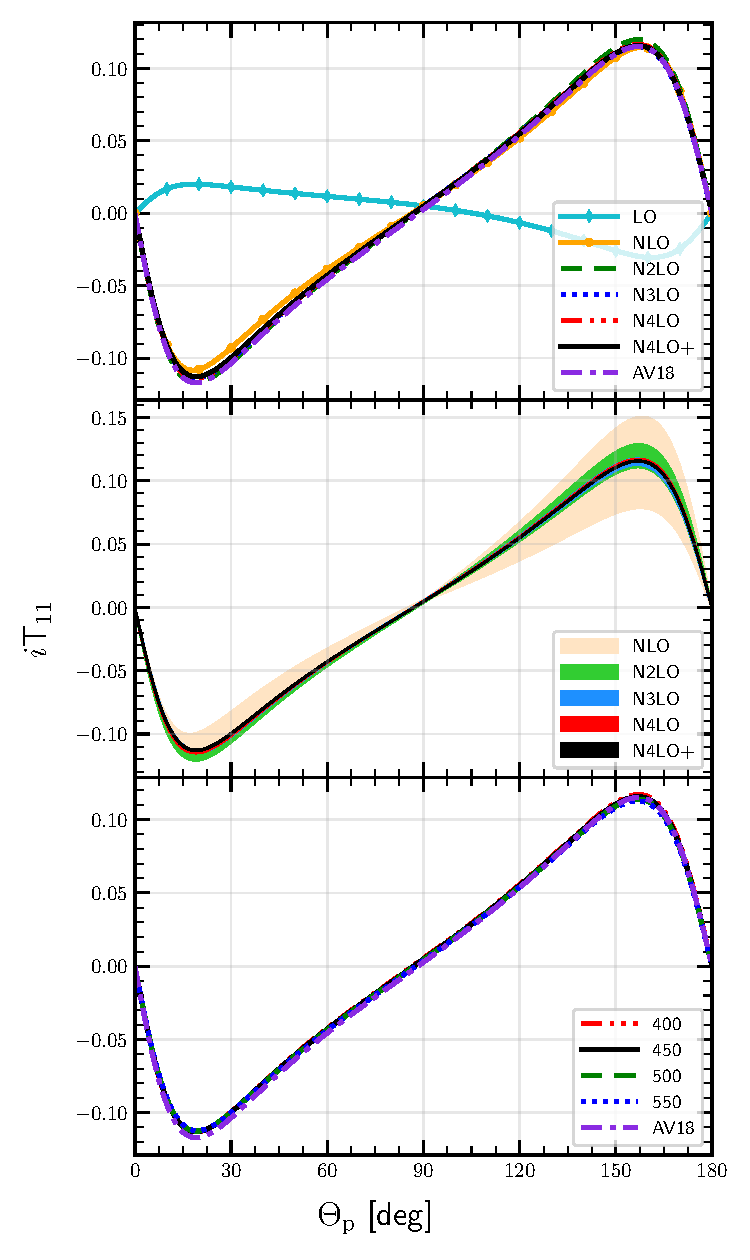
\includegraphics[width=\textwidth]{Figures_De/T11D2_30mev.pdf}
            \label{T11_30_vert}
        \end{subfigure}
        \caption{The same as in \fig{T20_T21_30} but for the deuteron tensor analyzing power
        T$_{22}$ (left column {\bf (a)}) and the deuteron vector analyzing power
        $i\text{T}_{11}$ (right column  {\bf (b)}).}
        \label{T22_T11_30}
    \end{figure}

    \begin{figure}[htb]
        \centering
        \begin{subfigure}[b]{0.46\textwidth}
            \caption{T$_{20}$}
            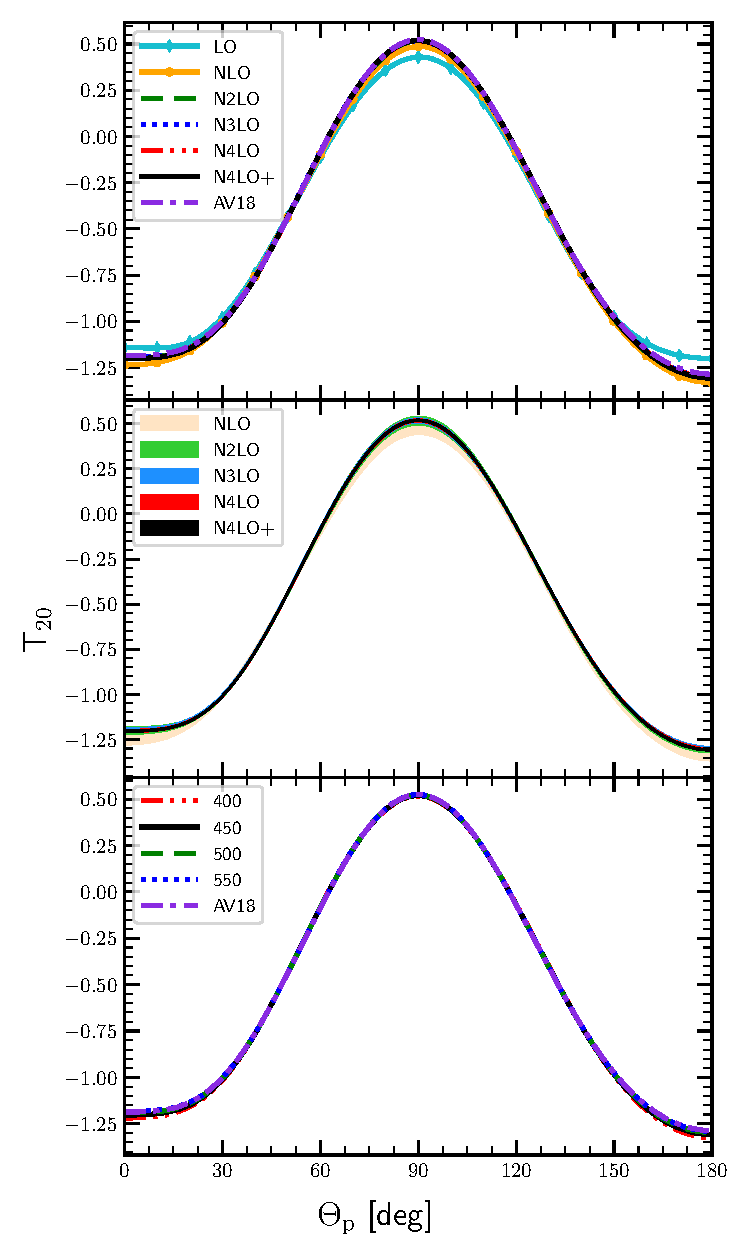
\includegraphics[width=\textwidth]{Figures_De/T20D2_100mev.pdf}
            \label{T20_100_vert}
        \end{subfigure}
        \begin{subfigure}[b]{0.46\textwidth}
            \caption{T$_{21}$}
            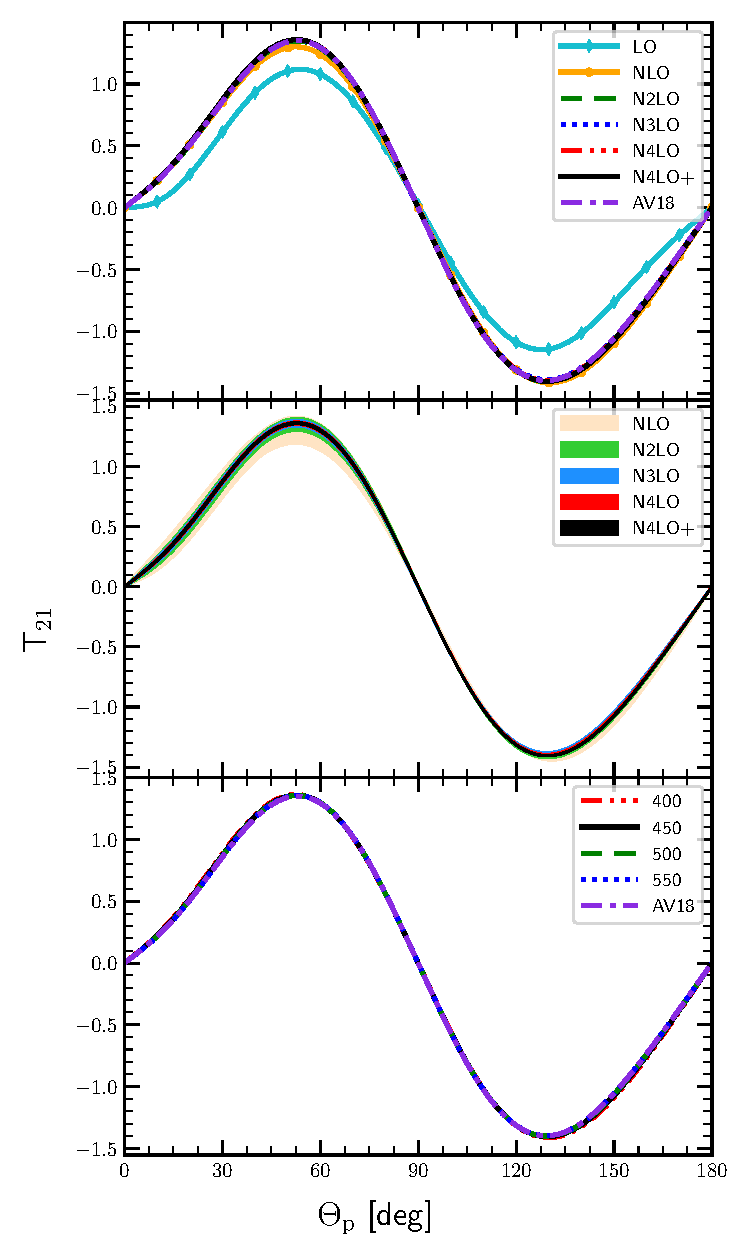
\includegraphics[width=\textwidth]{Figures_De/T21D2_100mev.pdf}
            \label{T21_100_vert}
        \end{subfigure}
        \caption{The deuteron tensor analyzing powers T$_{20}$  {\bf (a)}
        and T$_{21}$ {\bf (b)}
        as a function of the outgoing proton angle $\theta_p$ in the center of mass frame 
        for the photon energy E$_\gamma=\SI{100}{\mev}$.
        Top row presents results obtained using the \gls{sms} potential
        at different chiral orders (from \gls{lo} to \gls{n4lo+}) with the cut-off parameter $\Lambda=\SI{450}{\mev}$.
        The middle row shows truncation errors for each 
        chiral order starting from \gls{nlo} and the
        bottom row presents a cut-off dependence at \gls{n4lo+}.
        For the sake of comparison, predictions obtained with the \gls{av18} potential are given as well.
        For all predictions \gls{snc}+Siegert model is used.}
        \label{T20_T21_100}
    \end{figure}

    \begin{figure}[htb]
        \centering
        \begin{subfigure}[b]{0.46\textwidth}
            \caption{T$_{22}$}
            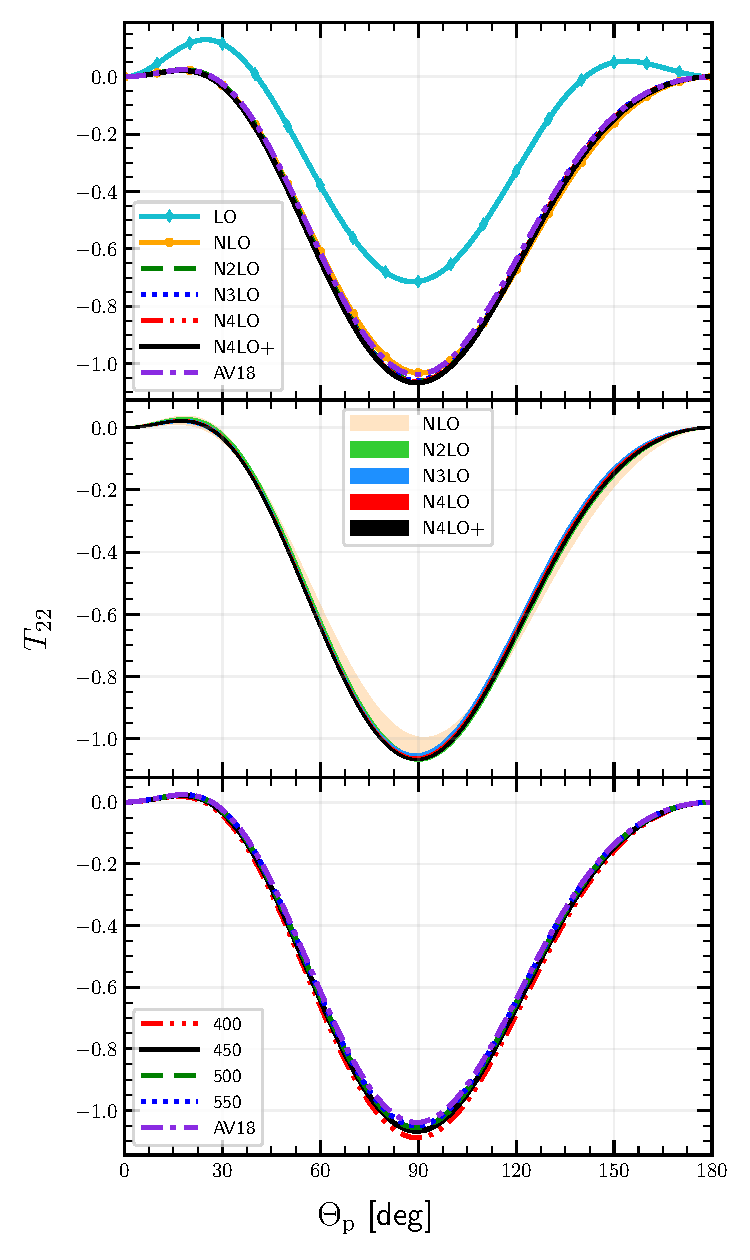
\includegraphics[width=\textwidth]{Figures_De/T22D2_100mev.pdf}
            \label{T22_100_vert}
        \end{subfigure}
        \begin{subfigure}[b]{0.46\textwidth}
            \caption{$i\text{T}_{11}$}
            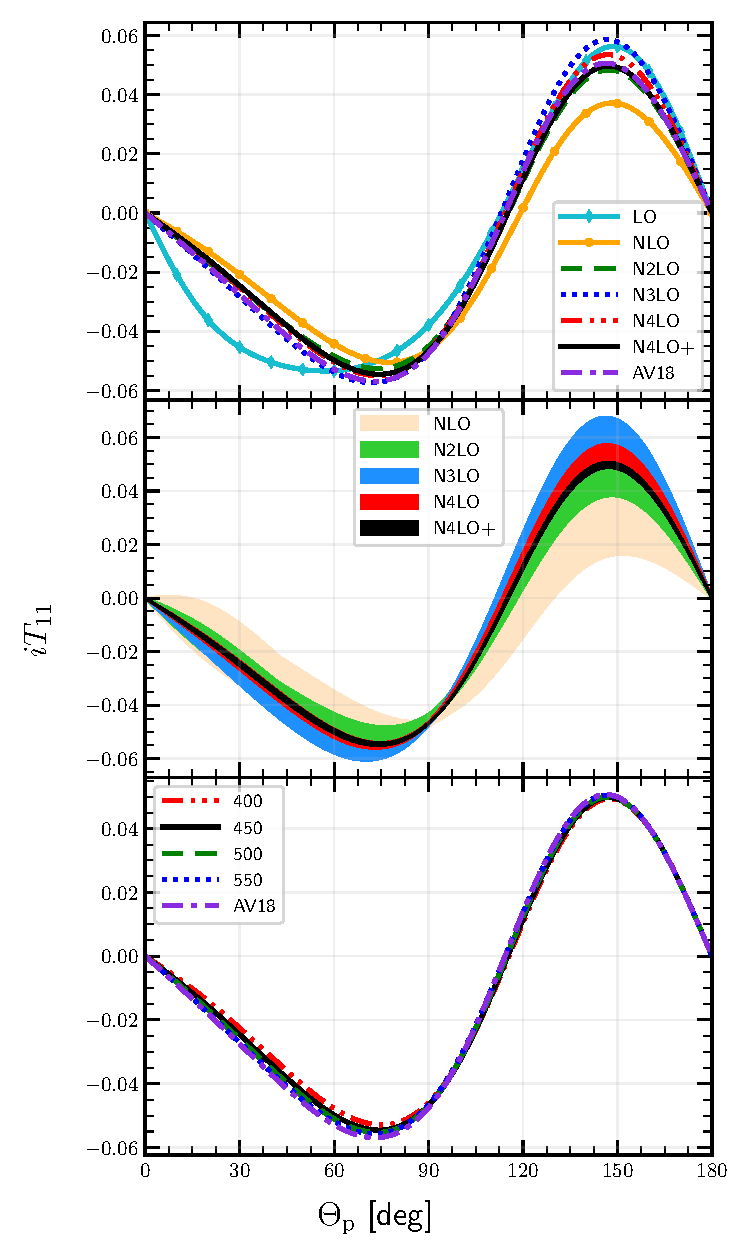
\includegraphics[width=\textwidth]{Figures_De/T11D2_100mev.pdf}
            \label{T11_100_vert}
        \end{subfigure}
        \caption{The same as in \fig{T20_T21_100} but for the deuteron tensor analyzing power
        T$_{22}$ (left column {\bf (a)}) and
        the deuteron vector analyzing power $i\text{T}_{11}$
        (right column {\bf (b)}).}
        \label{T22_T11_100}
    \end{figure}

    In \fig{tensor_pw_1nc} together with our most advanced "Full" predictions 
    (\gls{n4lo+}, $\Lambda=\SI{450}{\mev}$, the Siegert theorem),
    at $\text{E}_\gamma = \SI{30}{\mev}$ 
    I show predictions obtained with 1NC only and 
    the Siegert predictions but with plane-wave contribution without rescattering part.
    In the case of deuteron's tensor analyzing power components, the contribution of rescattering part is  
    imortant for T$_{20}$, T$_{21}$ and T$_{22}$ (the relative difference is up to \SI{20}{\percent} 
    in extremes).
    and crucial for
    $i\text{T}_{11}$ where the PW part equals to zero.
    The 2NC component taken into account via Siegert theorem has a dominant contribution here. We see that 
    1NC predictions are absolutely away from the "Full" predictions and in case of $i\text{T}_{11}$
    does not even reflect complete prediction qualitatively.

    \begin{figure}[h]
        \begin{center}
        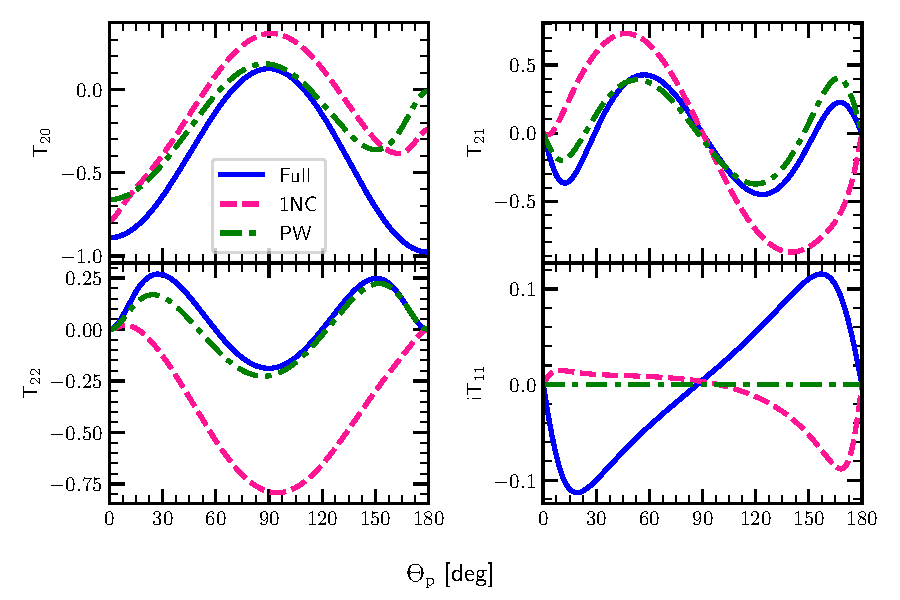
\includegraphics[width=0.9\textwidth]{Figures_De/TensorPowers_pw_1nc.pdf}
        \end{center}
        \caption{The deuteron tensor analyzing powers T$_{20}$, T$_{21}$, T$_{22}$ and 
        the deuteron vector analyzing power $i\text{T}_{11}$ as a function of the
        outgoing proton angle $\theta_p$ in the \gls{cm} frame at $\text{E}_\gamma = \SI{30}{\mev}$.
        Similarly to \fig{Diff_cross_pw_1nc} predictions obtained with chiral \gls{n4lo+} potential
        and $\Lambda=\SI{450}{\mev}$ are presented for three theoretical models.
        Blue solid line is the most complete prediction we have (plane-wave plus rescattering parts, 1NC + Siegert), pink dashed line shows predictions obtained with
        single-nucleon current only (1NC) - without the Siegert contributions and green dashed-dotted line
        is a prediction in which we neglect the rescattering part
        and stick to the plane-wave part only but keeping the Siegert contributions.}
        \label{tensor_pw_1nc}
    \end{figure}

    \fig{tensor_pw_1nc_100mev} presents similar results but for E$_\gamma = \SI{100}{\mev}$
    and it is intersting that the difference between Full and 1NC prediction becomes smaller
    and it is especially visible for $\text{T}_{22}$. At this energy the relative difference 
    between "Full" and 1NC predictions
    at $\theta_p = \ang{90}$ is \SI{43.6}{\percent} comparing to \SI{122.8}{\percent}
    at E$_\gamma = \SI{30}{\mev}$. Similarly, the difference for T$_{20}$
    at E$_\gamma = \SI{30}{\mev}$($\theta_p = \ang{90}$) is \SI{91.4}{\percent}
    and at E$_\gamma = \SI{100}{\mev}$ it drops to \SI{28.8}{\percent}.
    This may also be affected by the fact that values at $\theta_p = \ang{90}$ 
    are quit small for the Full prediction, nevertheless the difference still becomes smaller at the
    E$_\gamma = \SI{100}{\mev}$.
    This trend is noticeable looking also on results presented below.
    Nevertheless, in both cases 2NC (via the Siegert) bring sufficient contributions
    and cannot be omitted for the full picture.

    \begin{figure}[h]
        \begin{center}
        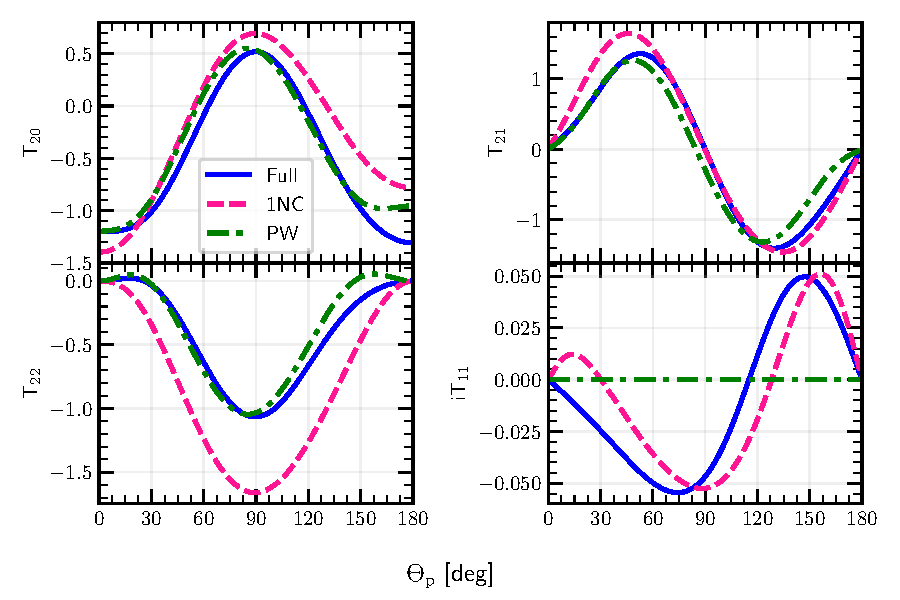
\includegraphics[width=0.9\textwidth]{Figures_De/TensorPowers_100mev_pw_1nc.pdf}
        \end{center}
        \caption{The same as in \fig{tensor_pw_1nc} but for E$_\gamma=\SI{100}{\mev}$.}
        \label{tensor_pw_1nc_100mev}
    \end{figure}

    
    In the following figures, I will compare my predictions with experimental data.
    In some cases I will keep a similar way as it was done
    in \cite{rachek2007} where due to experimental conditions results are given not at single photon energy,
    but for a specific ranges of $\text{E}_\gamma$.
    In the Figures \ref{tensor_angular_25-45} - \ref{tensor_angular_230-330}
    I show an angular dependence of the $\text{T}_{2i}$ ($i=0,1,2$) for a specific energy bands:
    \SIrange[range-phrase=--]{25}{45}{\mev}, \SIrange[range-phrase=--]{45}{70}{\mev},
    \SIrange[range-phrase=--]{70}{100}{\mev}, and \SIrange[range-phrase=--]{230}{330}{\mev}.
    Solid blue line shows an average value of the observable in the specified energy intervals:
    obtained at \gls{n4lo+} with $\Lambda=\SI{450}{\mev}$, while the pink dashed line is a prediction
    obtained with a same setup but without using a contributions from Siegert approach
    (single nucleon current only). Bands for each of prediction specify the spread of
    predictions due to the energy band.
    
    % \tmp{stick to either SN or 1NC(this one probably) ??}

    One clearly sees that the data description is better for the predictions with Siegert contributions included
    and the \gls{snc} alone is not able to describe experiment properly.
    Our Full model nicely describes data up to $\text{E}_\gamma = \SI{70}{\mev}$.
    With increasing energy (above \SI{100}{\mev}),
    the difference between predicted values and experimental data becomes larger
    (especially for $\text{T}_{22}$), 
    which shows a neccesity of improving theoretical model befor applying it to 
    higher energies. Nevertheless, even with approximations used,
    the data description remains reasonable. 
    We observe that quite often and in particular in \fig{tensor_angular_180-230} and \fig{tensor_angular_230-330}
    the data description is worse for smaller angles. Especially for the tensor analyzing power T$_{22}$
    the group of data point lying closer to $\theta_p = \ang{30}$ are farther 
    from the theoretical prediction than second group.
    In \fig{tensor_angular_230-330} the description of data points for T$_{20}$ seem to be better
    with the \gls{snc} (dashed line), but in this case it is only accidental match as we do not observe similar 
    trend for any other angular range or for different observable. 
    In addition, experimental uncertainties are larger at small angles and in all cases 
    our description is inside 3$\sigma$ uncertainty.
    




    \begin{figure}[h]
        \begin{center}
        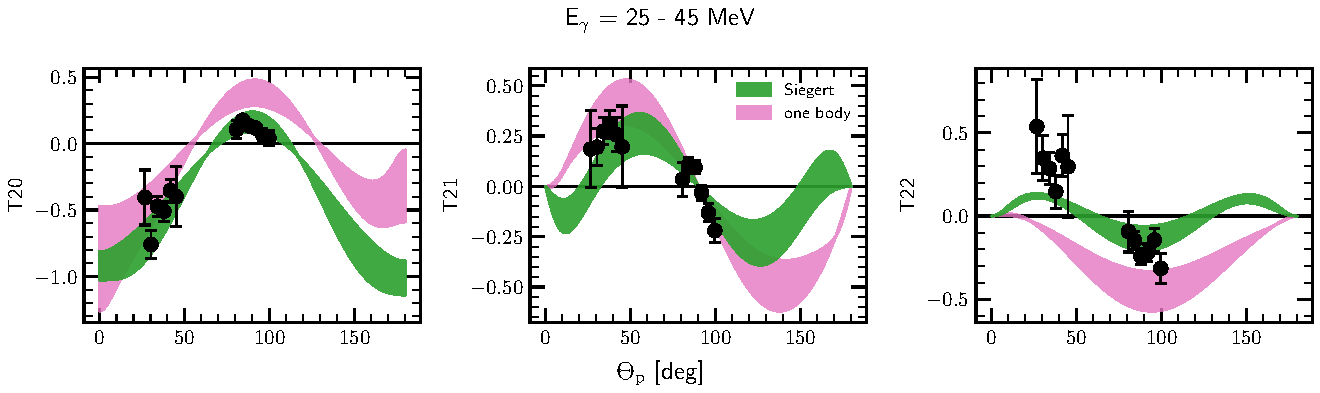
\includegraphics[width=1\textwidth]{Figures_De/Tensor_analyzing_power_angular_E25-45.pdf}
        \end{center}
        \caption{Tensor analyzing powers T$_{20}$, T$_{21}$ and T$_{22}$ as a function of the
        outgoing proton angle $\theta_p$ in the \gls{cm} frame.
        The solid blue line is a mean value of my predictions obtained 
        at energy values from \SIrange[range-phrase=\text{ to }]{25}{45}{\mev} with the
        \gls{sms} potential at \gls{n4lo+} chiral order and with $\Lambda$~=~450~MeV
         and with \gls{snc} used together with the Siegert approach. 
        The pink dashed line is similar prediction but with the \gls{snc} only. 
        The corresponding bands show the limits of predictions in the regarded
        energy region.
        % Filled bands show maximal spread of my predictions obtained with a 
        % \gls*{sms} potential at \gls{n4lo+} chiral order and with $\Lambda$~=~450~MeV
        % for the energy span from 25 to 45 MeV. Blue bands correspond to the
        % case where \gls{snc} was used together with Siegert approach and 
        % pink bands - to the \gls{snc}only. 
        Filled circles are experimental data
        from \cite{rachek2007} for the same energy range.}
        \label{tensor_angular_25-45}
    \end{figure}

    \begin{figure}[h]
        \begin{center}
        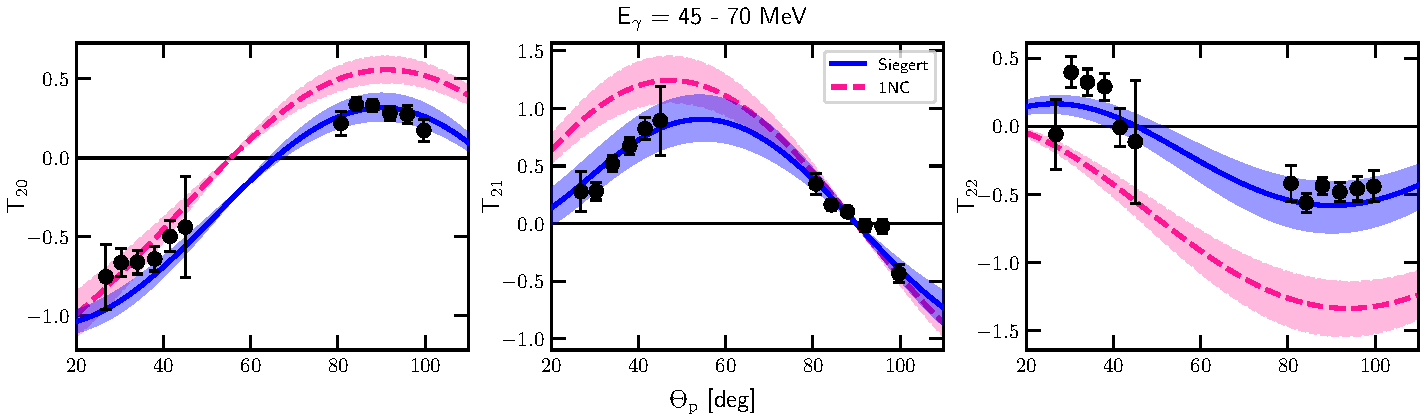
\includegraphics[width=0.95\textwidth]{Figures_De/Tensor_analyzing_power_angular_E45-70.pdf}
        \end{center}
        \caption{The same as in \fig{tensor_angular_25-45} but for energy bin \SIrange{45}{70}{\mev}.}
        \label{tensor_angular_45-70}
    \end{figure}

    \begin{figure}[h]
        \begin{center}
        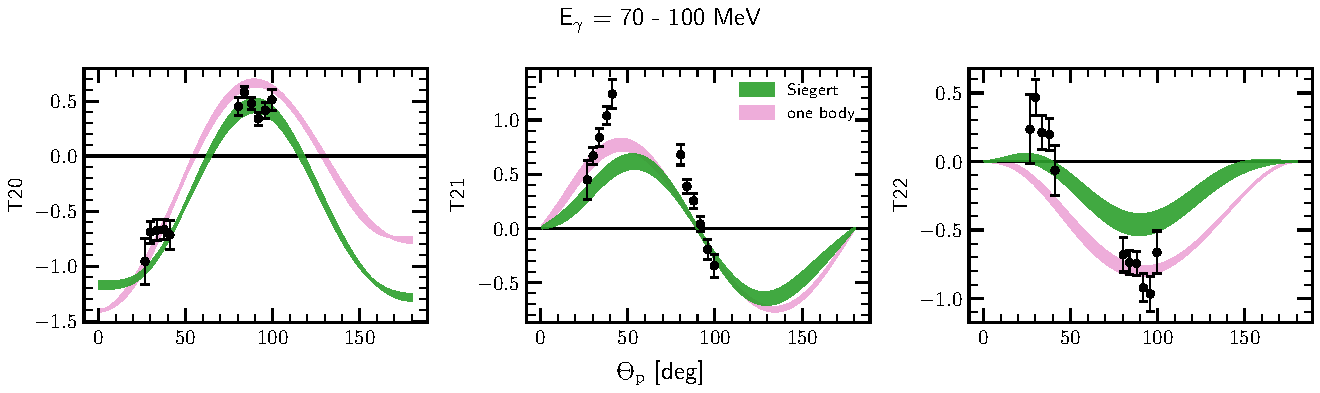
\includegraphics[width=0.95\textwidth]{Figures_De/Tensor_analyzing_power_angular_E70-100.pdf}
        \end{center}
        \caption{The same as in \fig{tensor_angular_25-45} but for energy bin \SIrange{70}{100}{\mev}.}
        \label{tensor_angular_70-100}
    \end{figure}        

    \begin{figure}[h]
        \begin{center}
        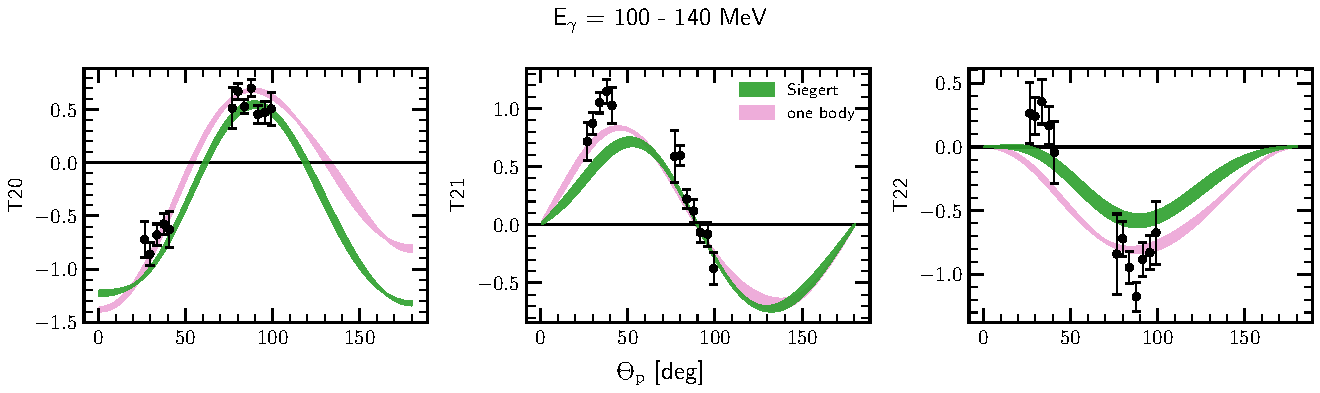
\includegraphics[width=0.95\textwidth]{Figures_De/Tensor_analyzing_power_angular_E100-140.pdf}
        \end{center}
        \caption{The same as in \fig{tensor_angular_25-45} but for energy bin \SIrange{100}{140}{\mev}.}
        \label{tensor_angular_100-140}
    \end{figure}
        
        

    \begin{figure}[h]
        \begin{center}
        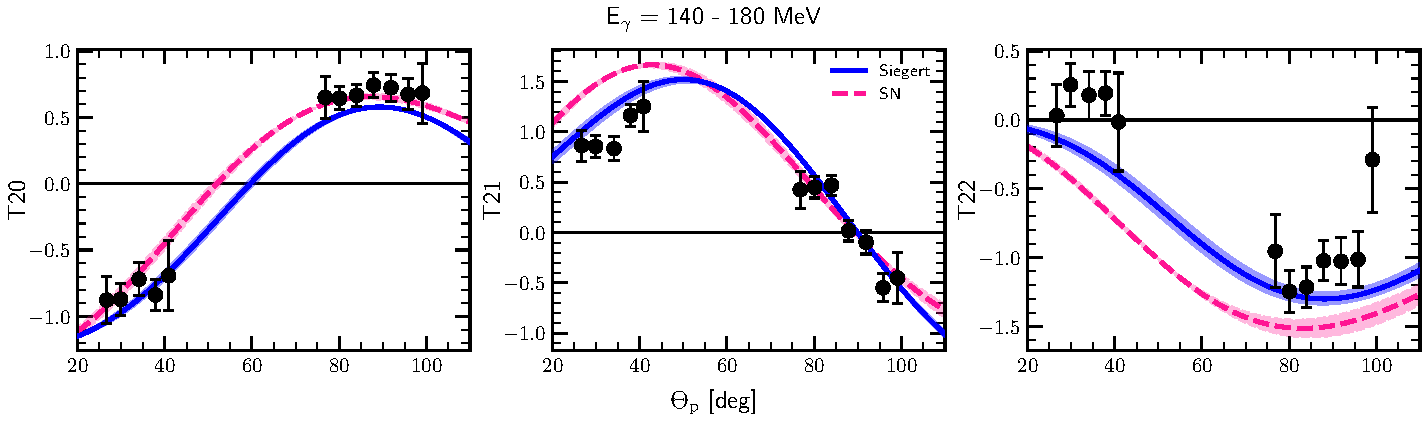
\includegraphics[width=0.95\textwidth]{Figures_De/Tensor_analyzing_power_angular_E140-180.pdf}
        \end{center}
        \caption{The same as in \fig{tensor_angular_25-45} but for energy bin \SIrange{140}{180}{\mev}}
        \label{tensor_angular_140-180}
    \end{figure}
        

    \begin{figure}[h]
        \begin{center}
        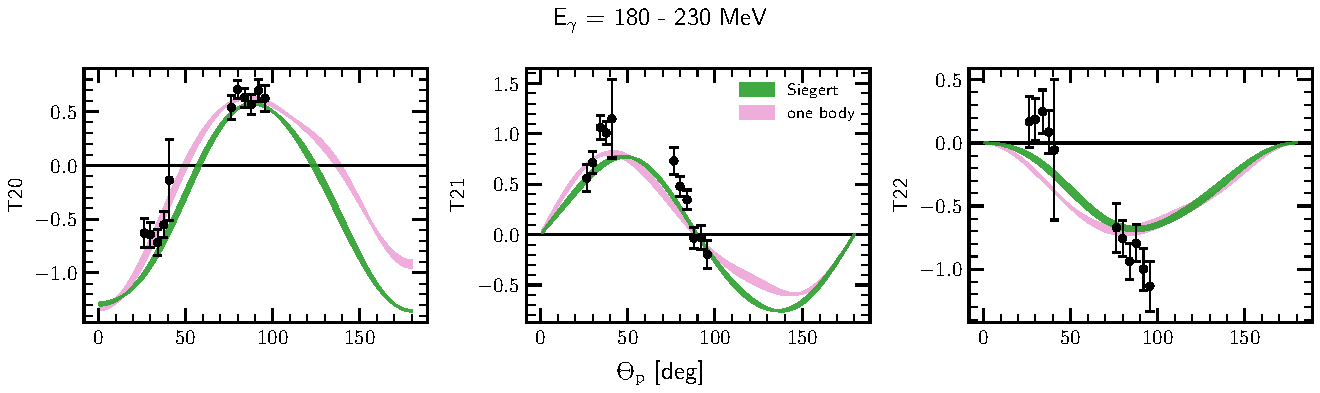
\includegraphics[width=0.95\textwidth]{Figures_De/Tensor_analyzing_power_angular_E180-230.pdf}
        \end{center}
        \caption{The same as in \fig{tensor_angular_25-45} but for energy bin \SIrange{180}{230}{\mev}}
        \label{tensor_angular_180-230}
    \end{figure}

    \begin{figure}[h]
        \begin{center}
        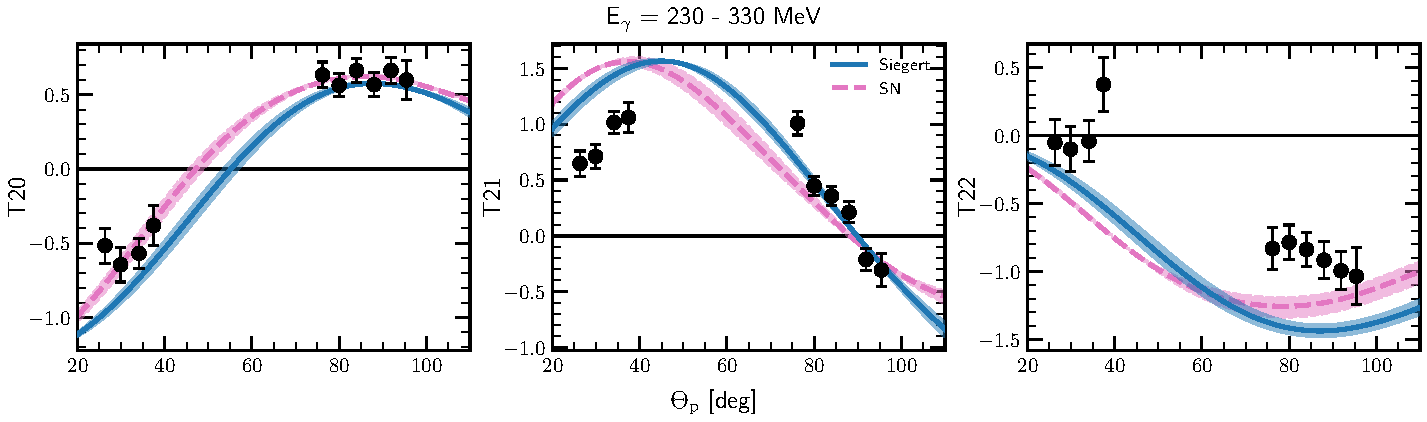
\includegraphics[width=0.95\textwidth]{Figures_De/Tensor_analyzing_power_angular_E230-330.pdf}
        \end{center}
        \caption{The same as in \fig{tensor_angular_25-45} but for energy bin \SIrange{230}{330}{\mev}}
        \label{tensor_angular_230-330}
    \end{figure}
        


    In the Figure \ref{T20_vs_en} the energy dependence of $\text{T}_{20}$ and $\text{T}_{22}$
    at specific angle $\theta_p = \ang{88}$
    is presented for the energy range 0-400~MeV. Beside my predictions I also demonstrate the experimental data from
    \cite{rachek2007} and \cite{mishev1993} as well as theoretical calculations from \cite{Schmitt1989}.
    For $\text{T}_{20}$ all models are able to describe experimental data well even for
    high energies. On the other hand, $\text{T}_{22}$ is not described so well: for the 
    energies below \SI{140}{\mev} the predictions are within uncertainties of experimental data,
    but further the difference with the data increases. Above \SI{140}{\mev}
    my Full predictions do not  
    reflect the qualitative nature of the data. Namely, I observe that
    data points start ascending which is not represented in my predictions.
    Theoretical predictions from \cite{Schmitt1989} (brown dashed curve) are also not able
    to describe data quantitatively for $\text{T}_{22}$, but increasing of T$_{22}$
    towards data is present. The predictions in \cite{Schmitt1989}
    are obtained with a one-body current using the Bonn one-boson-exchange potential
    in coordinate space (OBEPR)
    NN potential with the major part of meson exchange
    currents (MEC) included implicitly via the Siegert operators plus explicit
    pion exchange currents (MEC), isobar configurations
    (IC) and the leading order relativistic corrections
    (RC). So authors use a different potential, but
    probably the main difference of predictions is coming from the
    more advance model of the current operator
    and the RC included there.
    We see that experimental errors are quite large which is not so surprising
    giving that the experiment was conducted back in 1989.
    New experiments would be a great support in development of the nuclear interactions
    as we expect relativistic calculations in future \cite{Grassi2023}.

    The \fig{T20_vs_en_cutoff} presents similar results to the \fig{T20_vs_en} but
    with various values of the cutoff parameter. The deviation between these
    predictions is rather small (especially below \SI{150}{\mev}), while the
    difference with the calculation from \cite{Schmitt1989} and experimental 
    data remains as discussed above.

    Similar picture is seen in the Figures \ref{tensor_energy_24-48} and \ref{tensor_energy_70-102}
    where I show an energy dependence of the mean of deuteron analyzing powers over 
    specific angular ranges (following the data from \cite{rachek2007}).
    In \fig{tensor_energy_24-48} we see that only predictions for $\text{T}_{20}$
    are able to reflect the experimental results,
    while for $\text{T}_{21}$ and $\text{T}_{22}$ my results are reasonable (quantitative-wise) 
    only for lower energies and difference with data becomes larger
    when energy increases. Predictions for $\text{T}_{21}$ and $\text{T}_{22}$ once more 
    confirm an insufficiency of 1NC and an importance of
    2-nucleon current contributions.
    The description is better for bigger angles \fig{tensor_energy_70-102}):
    at lower energies (below \SI{140}{\mev}) the correspondence to
    experimental data is good for all three observables, but above that 
    threshold, all predictions (especially for $\text{T}_{22}$)
    move away from the measurements data.
    Again, big uncertainty of the data calls for experiment to be repeated.
    

    \begin{figure}[h]
        \begin{center}
        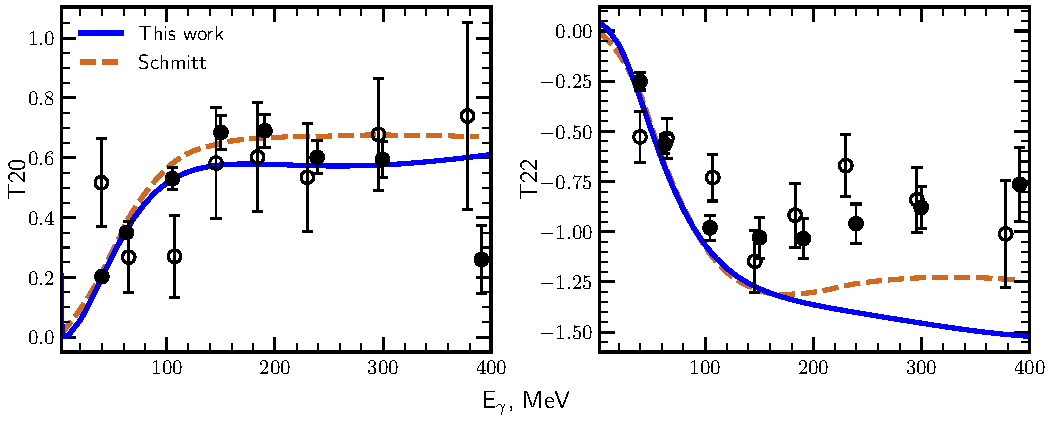
\includegraphics[width=0.9\textwidth]{Figures_De/T20_T22_vs_en.pdf}
        \end{center}
        \caption{
        The tensor analyzing powers T$_{20}$ (left) and T$_{22}$ (right) as
        a function of the photon energy E$_\gamma$
        at fixed outgoing proton angle $\theta_p = \ang{88}$ in the center of mass frame.
        My predictions (blue solid line) are obtained with the \gls{sms} potential at the chiral order \gls{n4lo+},
        with the cut-off parameter $\Lambda = \SI{450}{\mev}$ and with 2NC contributions included via the Siegert theorem.
        The dashed pink curve shows predictions obtained with the same interaction, but without 2NC contributions.
        The dashed-dotted brown curve presents theoretical results from \cite{Schmitt1989}.
        Experimental data are taken from \cite{rachek2007} (filled circles)
        and \cite{mishev1993} (empty circles).}
        \label{T20_vs_en}
    \end{figure}

    \begin{figure}[h]
        \begin{center}
        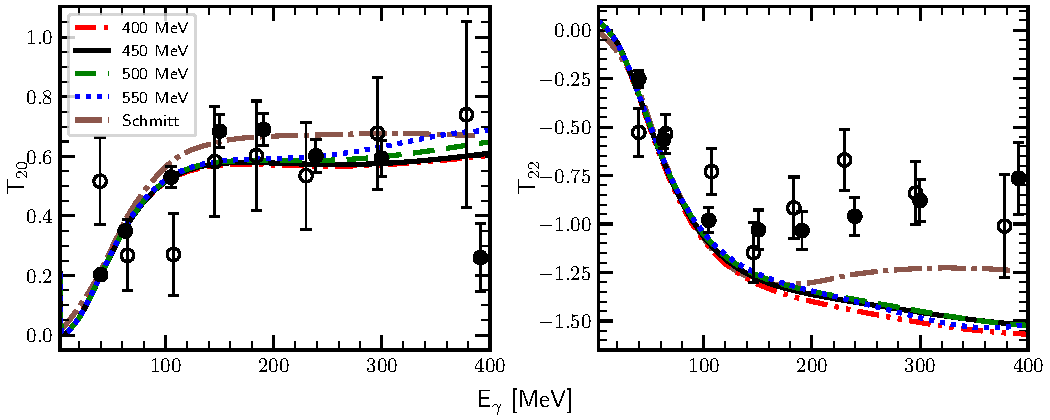
\includegraphics[width=0.9\textwidth]{Figures_De/T20_T22_vs_en_cutoff.pdf}
        \end{center}
        \caption{
        The tensor analyzing powers T$_{20}$ (left) and T$_{22}$ (right) as
        a function of the photon energy E$_\gamma$
        at fixed outgoing proton angle $\theta_p = \ang{88}$ in the center of mass frame.
        My predictions have been obtained with the \gls{sms} potential at the chiral order \gls{n4lo+},
        with the different values of the cut-off parameter $\Lambda$ (from \SI{400}{\mev} to \SI{550}{\mev}).
        The dashed-dotted brown curve presents theoretical results from \cite{Schmitt1989}.
        Experimental data are taken from \cite{rachek2007} (filled circles)
        and \cite{mishev1993} (empty circles).}
        \label{T20_vs_en_cutoff}
    \end{figure}

    \begin{figure}[h]
        \begin{center}
        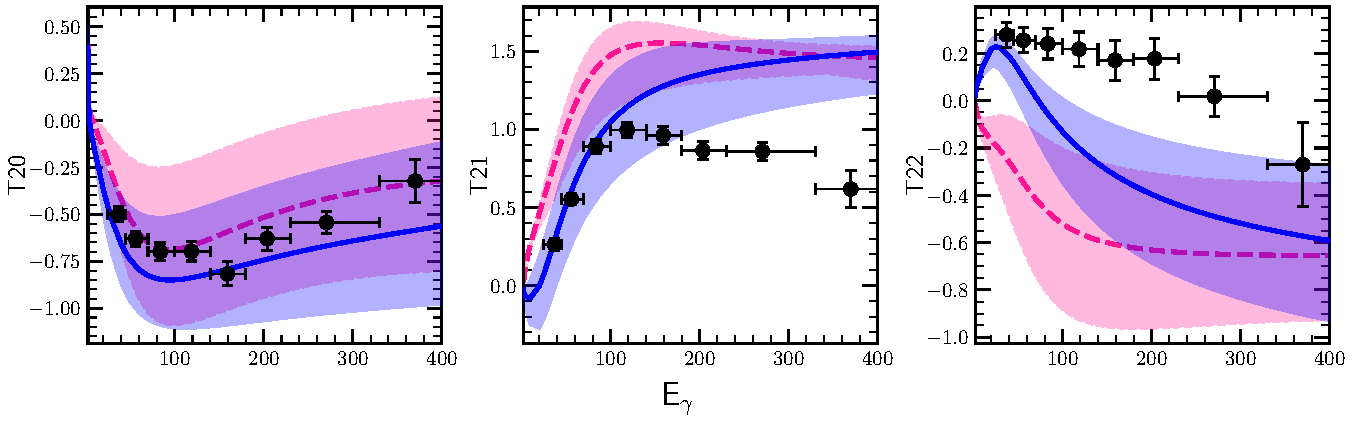
\includegraphics[width=0.95\textwidth]{Figures_De/TensorPower_Th24-48.pdf}
        \end{center}
        \caption{The averaged tensor analyzing powers T$_{20}$ (left),
        T$_{21}$ (middle) and T$_{22}$ (right) as a function of the
        photon energy for the outgoing proton momentum polar angle $\theta_p$
        in range $\ang{24} - \ang{48}$ in the center of mass frame.
        The solid blue curve is a mean value of my predictions at energy values ranges
        from 25 to \SI{45}{\mev}, obtained with
        the \gls{sms} potential at \gls{n4lo+} chiral order and with $\Lambda=\SI{450}{\mev}$
        and with \gls{snc} used together with the Siegert approach. 
        The pink dashed curve represents similar predictions but with
        the nuclear current reduced to the \gls{snc} only. 
        The corresponding bands show predictions at border energies 25 and \SI{45}{\mev}.
        The filled circles are experimental data
        from \cite{rachek2007} for the same energy range.}
        \label{tensor_energy_24-48}
    \end{figure}

    \begin{figure}[h]
        \begin{center}
        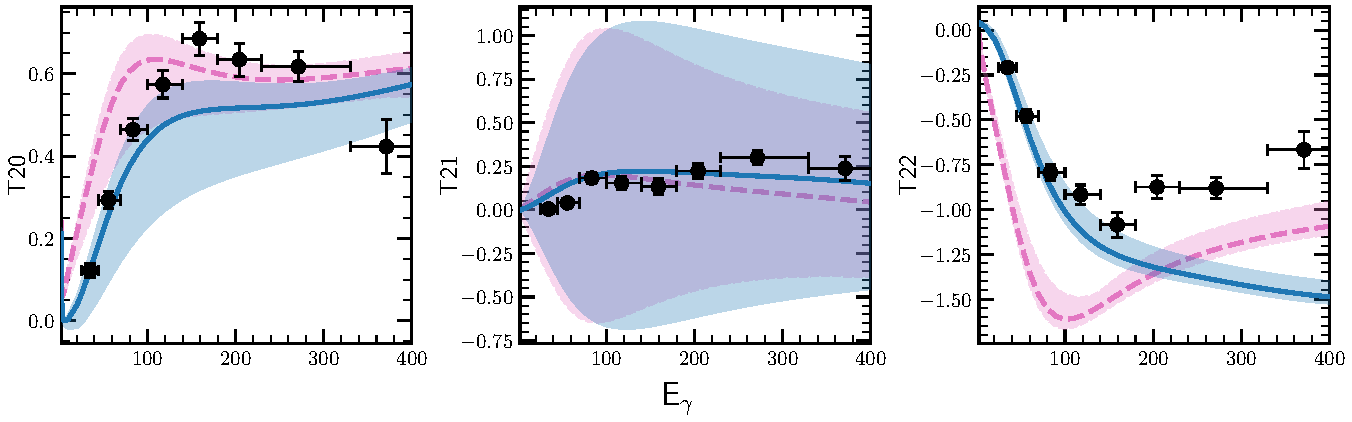
\includegraphics[width=0.95\textwidth]{Figures_De/TensorPower_Th70-102.pdf}
        \end{center}
        \caption{The same as in the \fig{tensor_energy_24-48} but
        for the $\theta_p$ in range $\ang{70} - \ang{102}$.}
        \label{tensor_energy_70-102}
    \end{figure}
    
    In the \fig{assymetry} I demonstrate predictions
    for the photon asymmetry $\Sigma_\gamma$ for the 
    deuteron photodisintegration with $\text{E}_\gamma=\SI{20}{\mev}$ (a)
    and \SI{60}{\mev}(b) together with the experimental data of 
    \cite{KRAUSE1992_asymetry, depascale_asymmetry, Barannik_asymetry, Vnukov_asymmetry}.
    Both (a) and (b) figures are organized similarly to the 
    figures I showed above for the tensor analyzing powers (e.g. \fig{T22_T11_30}).
    That is the top panel is aimed to demonstrate predictions obtained
    with the chiral \gls{sms} potential at different orders of the chiral expansion,
    the middle one is showing a truncation errors and the bottom one shows 
    the cut-off dependence. For that observable we see an excellent 
    convergence with respect to the chiral order. For both regarded 
    energies predictions at different orders are very close to each other
    except the \gls{lo} and \gls{nlo} curves. Nevertheless, at E$_\gamma = \SI{60}{\mev}$
    the truncation error bands reveal some uncertainty connected 
    with the chiral order and it is expected that even some higher chiral 
    orders would still contribute to the predictions at this energy.
    The relative width of the truncation band are 
    \SIlist{0.26;5.04;5.05;5.73;14.96}{\percent} for \gls{n4lo+}, \gls{n4lo}, \gls{n3lo},
    \gls{n2lo} and \gls{nlo} respectively and at $\theta_p=\ang{90}$.

    The cut-off dependence is also much stronger at \SI{60}{\mev}. One clearly sees
    that predictions are different for various values of the $\Lambda$.
    The relative difference between predictions to the cut-off parameter at \SI{20}{\mev}
    is \SI{0.26}{\percent} while at the photon energy \SI{60}{\mev}
    it is  \SI{4.41}{\percent} (both calculated at $\theta_p=\ang{90}$).
    So the theoretical uncertainty related to regulator value
    is nearly 17 times bigger that due to the truncation error ($4.11/0.26 = 16.96$).

     Comparing my predictions to experimental data, I observe that
     for the lower energy predictions are almost perfectly overlapping
     with experimental points within the error bars. 
     For a few data points our predictions are
     outside data error bars, but they are still within $3\sigma$ range.
     For \SI{60}{\mev}, experimental data points are systematically below theoretical
     curves, especially in the middle of angular range. It seems that some systematic 
     uncertainty is presented in predictions and ad hoc multiplication by some factor
     (around 0.8)
     could help predictions be more similar to experimental data. But very likely the observed discrepancy
     points to simplified character of the model used here.

     In the \fig{asymmetry_energy_1NC} the predictions obtained with Full set of
     components (plane wave + rescattering and \gls{snc} + Siegert, solid blue curve) are shown
     versus predictions obtained without rescattering (green dashed-dotted line)
     and without contribution from the Siegert (pink dashed line) for the same 
     photon energies as above: E$_\gamma=\SI{20}{\mev}$ (left panel)
     and E$_\gamma=\SI{60}{\mev}$ (right panel).
     For the E$_\gamma=\SI{20}{\mev}$ the difference between Full and PW
     is quit small, whereas \gls{snc} is noticeably differs from the Full prediction,
     especially around the smallest and largest angle values.
     For the E$_\gamma=\SI{60}{\mev}$ the difference between such a predictions 
     is larger: we see not only quantitative, but also a qualitative variations.
     The \gls{snc} curve has much larger values and its shape becomes 
     more asymmetric with respect to the $\theta_p = \ang{90}$ point.

     In the \fig{asymmetry_90deg} (left) I present a dependence of the photon asymmetry
     $\Sigma_\gamma$ on the photon energy at a fixed value
     of the outgoing proton polar direction $\theta_p = \ang{90}$ 
     (following the data given at \cite{delbianco_1981} and \cite{depascale_asymmetry}).
     It is noticeable that with increasing energy, the predictions
     are systematically above the experimental data and the discrepancy growths with energy.
     This trend
     was also observed in the angular dependence of the asymmetry at \SI{60}{\mev}
     so I conclude that within our framework, 
     $\Sigma_\gamma$ is sensitive to the initial photon energy and some theoretical
     contributions are missing in order to get satisfactory predictions
     at higher energies. From the \fig{asymmetry_90deg} we can say that
     large discrepancy with data starts already above $\text{E}_\gamma = \SI{35}{\mev}$.
     \footnote{It is worth to note that data of \cite{depascale_asymmetry} are
     above these from \cite{delbianco_1981} (however still inside $3\sigma$ experimental
     error bands) and remain in agreement with my predictions even at E$_\gamma=\SI{60}{\mev}$.}

    The right panel of the \fig{asymmetry_90deg} shows an impact of the
    different model components to the obtained predictions.
    We see that the difference between the Full predictions (solid blue line)
    and the one obtained with a \gls{snc} only (without the Siegert contribution)
    is larger than the difference with predictions with plane-wave part only (without rescattering).
    Both these incomplete predictions are farther from the experimental data,
    (for PW at larger energies only) and have a different curve shape as well. 

    \begin{figure}[h]
        \centering
        \begin{subfigure}[b]{0.46\textwidth}
            \caption{\small E$_\gamma = \SI{20}{\mev}$}
            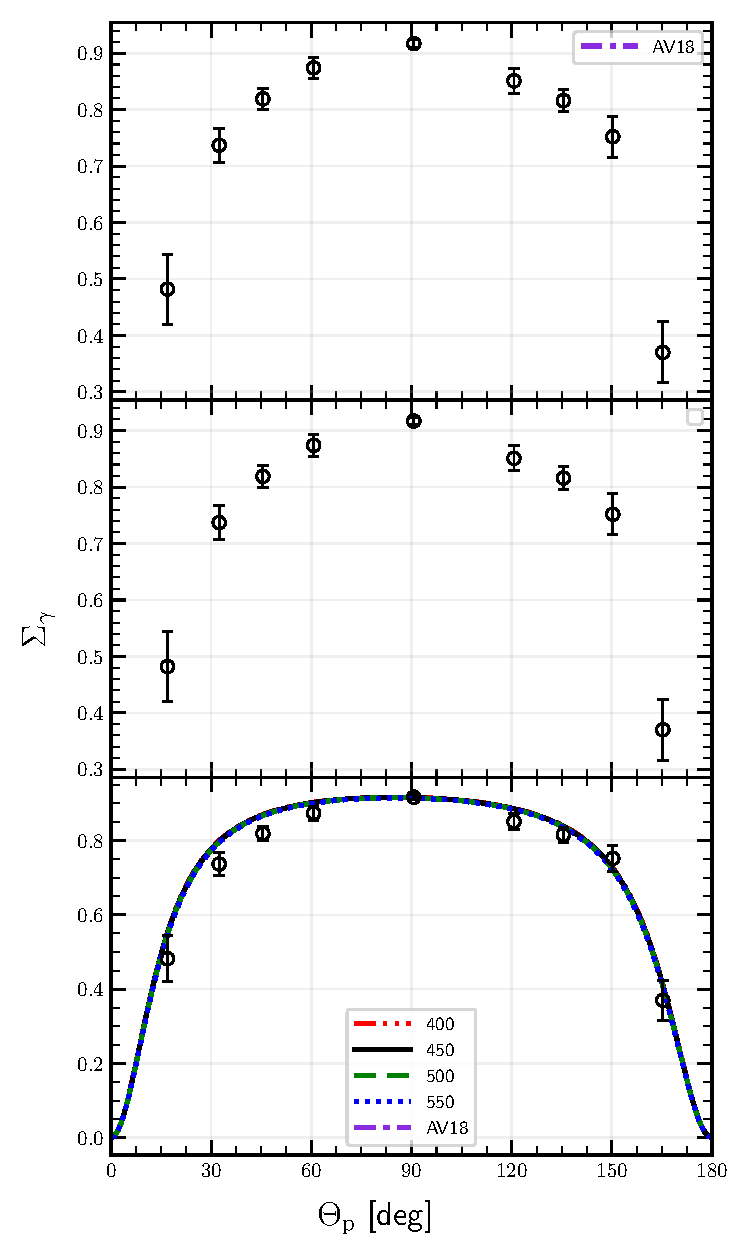
\includegraphics[width=\textwidth]{Figures_De/AX2_20mev.pdf}
            \label{AX_20_vert}
        \end{subfigure}
        \begin{subfigure}[b]{0.46\textwidth}
            \caption{\small E$_\gamma = \SI{60}{\mev}$}
            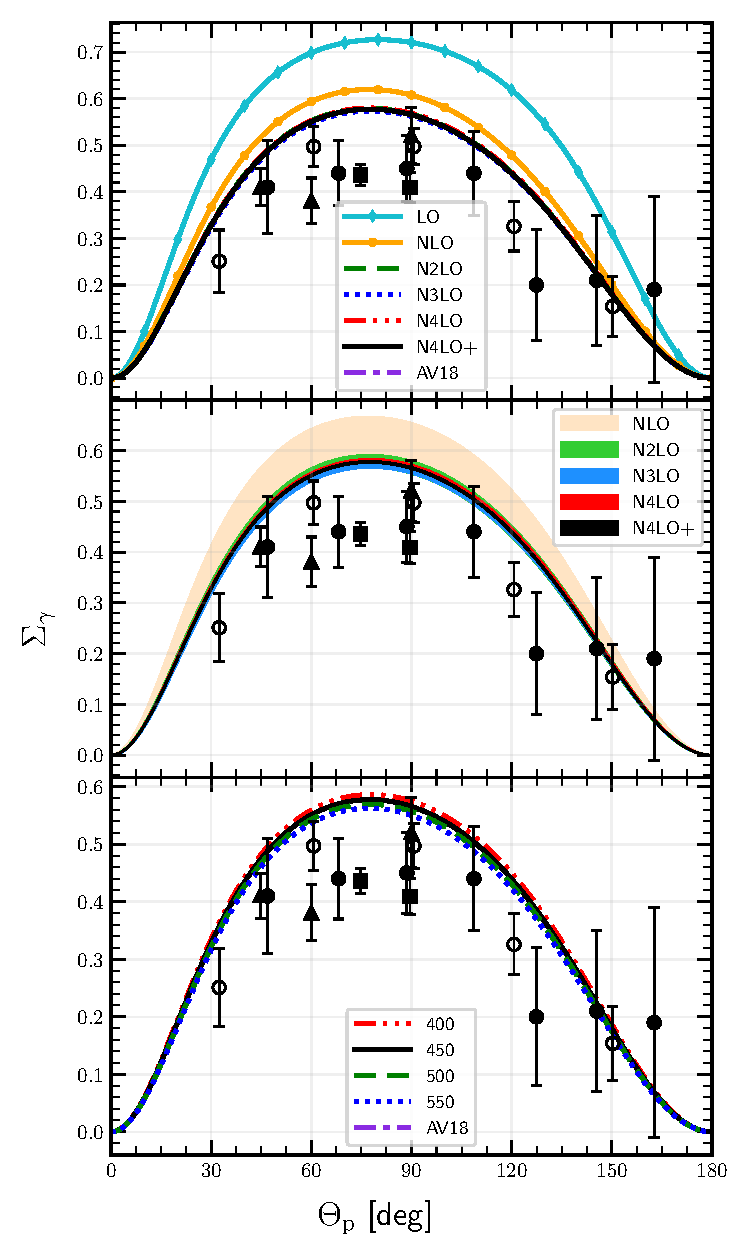
\includegraphics[width=\textwidth]{Figures_De/AX2_60mev.pdf}
            \label{AX_60_vert}
        \end{subfigure}
        \caption{The photon asymmetry $\Sigma_\gamma$ 
        as a function of the outgoing proton angle in the center of mass frame 
        for the photon energy \SI{20}{\mev}(a) and \SI{60}{\mev}(b).
        Top row presents results obtained using the \gls{sms} potential
        with chiral orders from \gls{lo} to \gls{n4lo+} and with the cut-off parameter $\Lambda=\SI{450}{\mev}$.
        The middle row shows truncation errors for each 
        chiral order starting from NLO and the
        bottom row presents a cut-off dependence for the chiral potential \gls{n4lo+}.
        Filled circles are experimental data from \cite{KRAUSE1992_asymetry},
        empty circles - from \cite{depascale_asymmetry}, filled squares
        - from \cite{Barannik_asymetry} and triangles are from \cite{Vnukov_asymmetry}.
        For the sake of comparison, predictions obtained with the \gls{av18} potential are
        given by the dashed-dotted curve as well.}
        \label{assymetry}
    \end{figure}


    \begin{figure}[h]
        \begin{center}
        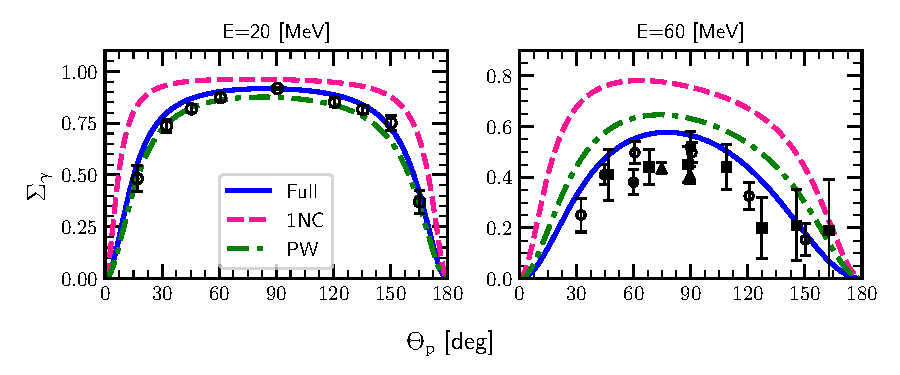
\includegraphics[width=0.95\textwidth]{Figures_De/Asymetry_20-60mev_pw_1nc.pdf}
        \end{center}
        \caption{The photon asymmetry $\Sigma_\gamma$ as a function of the
        outgoing proton angle $\theta_p$ in the \gls{cm} frame at $\text{E}_\gamma = \SI{20}{\mev}$
        (left) and $\text{E}_\gamma = \SI{60}{\mev}$(right).
        Similarly to \fig{Diff_cross_pw_1nc} predictions obtained with chiral \gls{n4lo+} potential
        and $\Lambda=\SI{450}{\mev}$ are presented for three theoretical models.
        Blue solid line is the most complete prediction we have (plane-wave plus rescattering parts, 1NC + Siegert), pink dashed line shows predictions obtained with
        single-nucleon current only (1NC) - without the Siegert contributions and green dashed-dotted line
        is a prediction in which we neglect the rescattering part
        and stick to the plane-wave part only but keeping the Siegert contributions.
        Filled circles are experimental data from \cite{KRAUSE1992_asymetry},
        empty circles - from \cite{depascale_asymmetry}, filled squares
        - from \cite{Barannik_asymetry} and triangles are from \cite{Vnukov_asymmetry}.}
        \label{asymmetry_energy_1NC}
    \end{figure}

     
    \begin{figure}[h]
        \begin{center}
        % 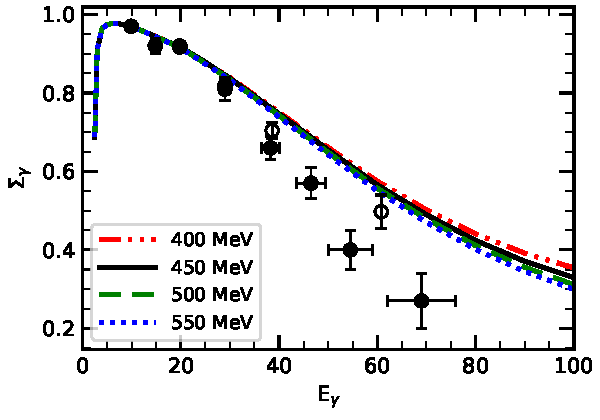
\includegraphics[width=0.75\textwidth]{Figures_De/AX2_90deg.pdf}
        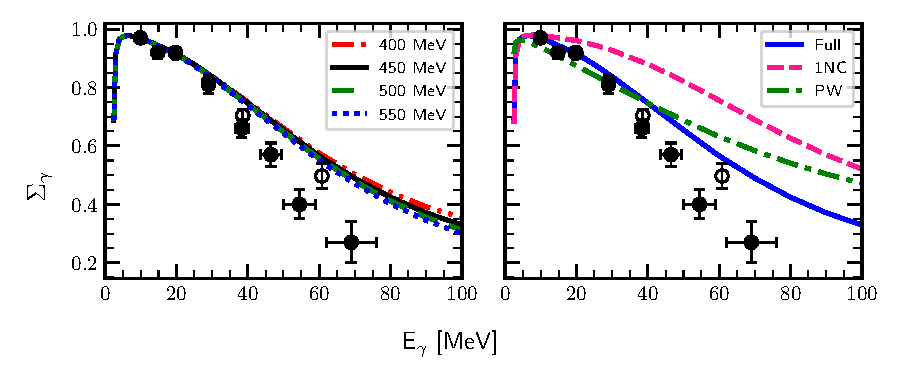
\includegraphics[width=0.95\textwidth]{Figures_De/AX2_90deg_1NC_PW.pdf}
        \end{center}
        \caption{The photon asymmetry $\Sigma_\gamma$ 
        as a function of the photon energy  
        at the fixed outgoing proton's momentum polar angle $\theta_p=90^\circ$.
        On the left panel each curve corresponds to the particular value of the cut-off parameter
        and chiral potential used here is the \gls{n4lo+} one.
        On the right panel the blue solid curve represents our most complete predictions
        comprising the plane-wave plus rescattering parts and \gls{snc}+Siegert current propagator 
        (the same as \SI{450}{\mev} line in left).
        The pink dashed curve shows predictions obtained with
        the single-nucleon current only (without applying the Siegert theorem) and the green dashed-dotted
        curve represents predictions with the full current (\gls{snc} + Siegert) but plane-wave part only.
        Filled circles are experimental data from \cite{delbianco_1981},
        empty circles - from \cite{depascale_asymmetry}.}
        \label{asymmetry_90deg}
    \end{figure}


    The proton polarization is demonstrated in \fig{PY_30_100_vert} for the 
    photon energy \SI{30}{\mev}(a) and \SI{100}{\mev}(b).
    In this case even at higher energy
    (such as \SI{100}{\mev}) predictions do not reveal neither
    slower convergence with respect to the chiral order no
    stronger cut-off dependence. Figures for both energies show
    that only next-to-leading order brings relatively high contribution
    while taking into account other subsequent orders does not change predictions
    significantly. In the case of the cut-off dependence, we see that curves for each
    value of $\Lambda$ are very close to each other. 
    The relative difference of the predictions with respect to the cut-off parameter
    is \SI{4.04}{\percent} at the minimum point $\theta_p=\ang{130}$ of $\text{E}_\gamma = \SI{30}{\mev}$
    and \SI{5.62}{\percent} at $\theta_p=\ang{160}$ and $\text{E}_\gamma = \SI{100}{\mev}$.
    The dependence is slightly stronger for higher energy, but both values are comparable.
    Again, the cut-off-related uncertainty exceeds the truncation error.

    \begin{figure}[h]
        \centering
        \begin{subfigure}[b]{0.46\textwidth}
            \caption{\small E$_\gamma = 30$~MeV}
            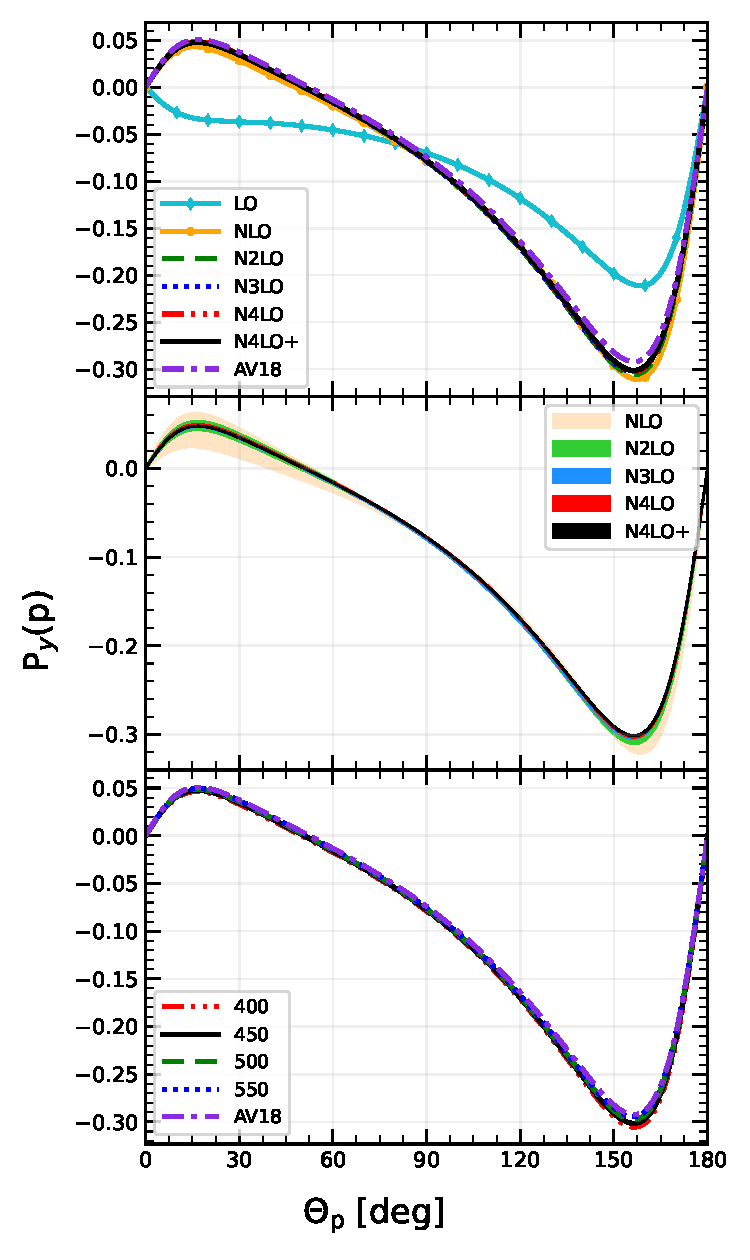
\includegraphics[width=\textwidth]{Figures_De/POLNOUT2(y)_30mev.pdf}
            \label{PY_30_vert}
        \end{subfigure}
        \begin{subfigure}[b]{0.46\textwidth}
            \caption{\small E$_\gamma = 100$~MeV}
            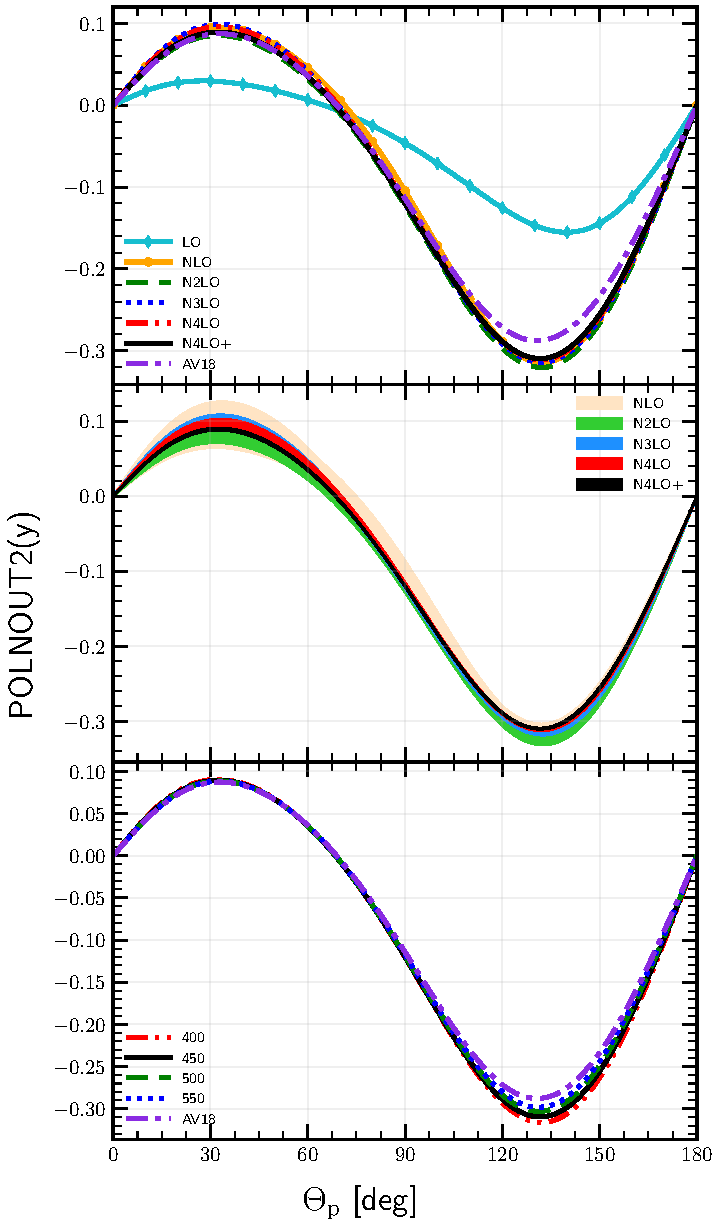
\includegraphics[width=\textwidth]{Figures_De/POLNOUT2(y)_100mev.pdf}
            \label{PY_100_vert}
        \end{subfigure}
        \caption{Proton polarization $P_y(p)$ 
        \label{PY_30_100_vert}
        as a function of the outgoing proton's momentum polar angle in the center of mass frame 
        with the photon energy \SI{30}{\mev} (a) and \SI{100}{\mev} (b).
        Top figures present results obtained using potential
        with different chiral orders (from \gls{lo} to \gls{n4lo+}) with cut-off parameter $\Lambda=\SI{450}{\mev}$.
        The middle panel show truncation errors for each 
        chiral order starting from \gls{nlo} and
        bottom figures present a cut-off dependence of predictions
        based on the \gls{sms} \gls{n4lo+} potential.
        For the sake of comparison, predictions obtained with the \gls*{av18} potential 
        are shown as well.}
    \end{figure}



    Predictions for the neutron polarization at the energies \SI{2.75}{\mev} and \SI{100}{\mev} are shown in the
    \fig{Pn_2p75_100}. The choice of energy is conditioned by the availability of experimental data,
    which were taken in 1965 in Livermore \cite{Jewell_neuteronpolarization} and 
    in 1986 at TRIUMF facility \cite{CAMERON_neuteronpolarization}.
    In the case of E$_\gamma = \SI{2.75}{\mev}$ (\fig{Pn_2p75_vert}), we see that predictions reflect
    the behavior of experimental data points qualitatively,
    having more o less a constant offset of the values. Similar offset was obtained
    also in \cite{ArenhovelPhotodisint1991}, where various approaches  were presented.
    Authors compare different models which leads to a very similar theoretical results
    even though different potentials are used with and without relativistic correction.
    One of the theoretical predictions is included even in the experimental papers
    \cite{Jewell_neuteronpolarization} and authors state that there might be a
    systematic error in the calibration of the analyzing power
    of the neutron polarimeter which could affect experimental results precision.
    Interesting is that predictions clearly show symmetrical form of the curve, while the experimental data
    have some deviations from symmetrical form. It can be a sign that some problem with data can be
    in this case (taking into account also that experiment had been done in 1965).
    In \cite{Jewell_neuteronpolarization} authors even make a plot of theoretical curve
    multiplied by the factor 0.879 which is almost perfectly overlaps with experimental data afterwards. 

    At the energy E$_\gamma = \SI{100}{\mev}$ (\fig{Pn_100_vert}) 
    my predictions describe the data very well.
    For most of data points, predicted values are within error bars and only some
    of points (e.g. around \ang{50}) have prediction in distance more than one standard deviation.
    Nevertheless, these data points look like being out of general trend and may be
    a result of imprecise measurement.
    Observing the stability of my predictions on the chiral order and regulator value I 
    conclude that nucleon polarizations are not the observables, which, even measured with much
    better precision, than it was done in \cite{Jewell_neuteronpolarization} or \cite{CAMERON_neuteronpolarization}
    would be an indicator of the model convergence or stability.

    Concluding my results of the deuteron photodisintegration predictions, 
    I can point that predictions for $\text{E}_\gamma = \SI{30}{\mev}$ (and lower)
    are very stable with respect to the potential parameters (chiral order or the regulator).
    It shows an ability for a good data description as well. For a higher energies (especially above \SI{100}{\mev})
    the quality of predictions becomes lower: the dependency on the cut-off value is higher as well as 
    discrepancy with experimental data. Still predictions are converged with respect to the chiral order.
    The general problem is a lack of 2N current and in case of higher energies - relativistic corrections are missing. 


    \begin{figure}[h]
        % \centering
        % 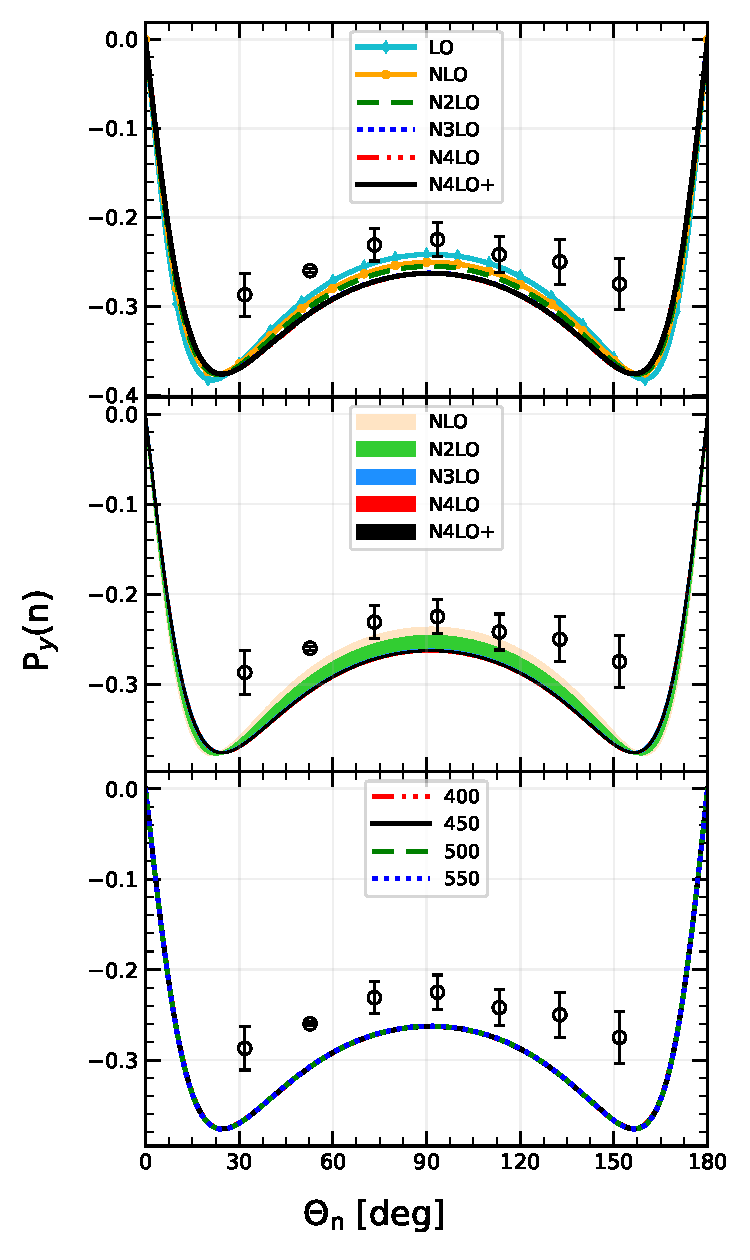
\includegraphics[width=0.5\textwidth]{Figures_De/POLNOUT2(y)_2.75mev_neuteron.pdf}
        \centering
        \begin{subfigure}[b]{0.46\textwidth}
            \caption{\small E$_\gamma = 2.75$~MeV}
            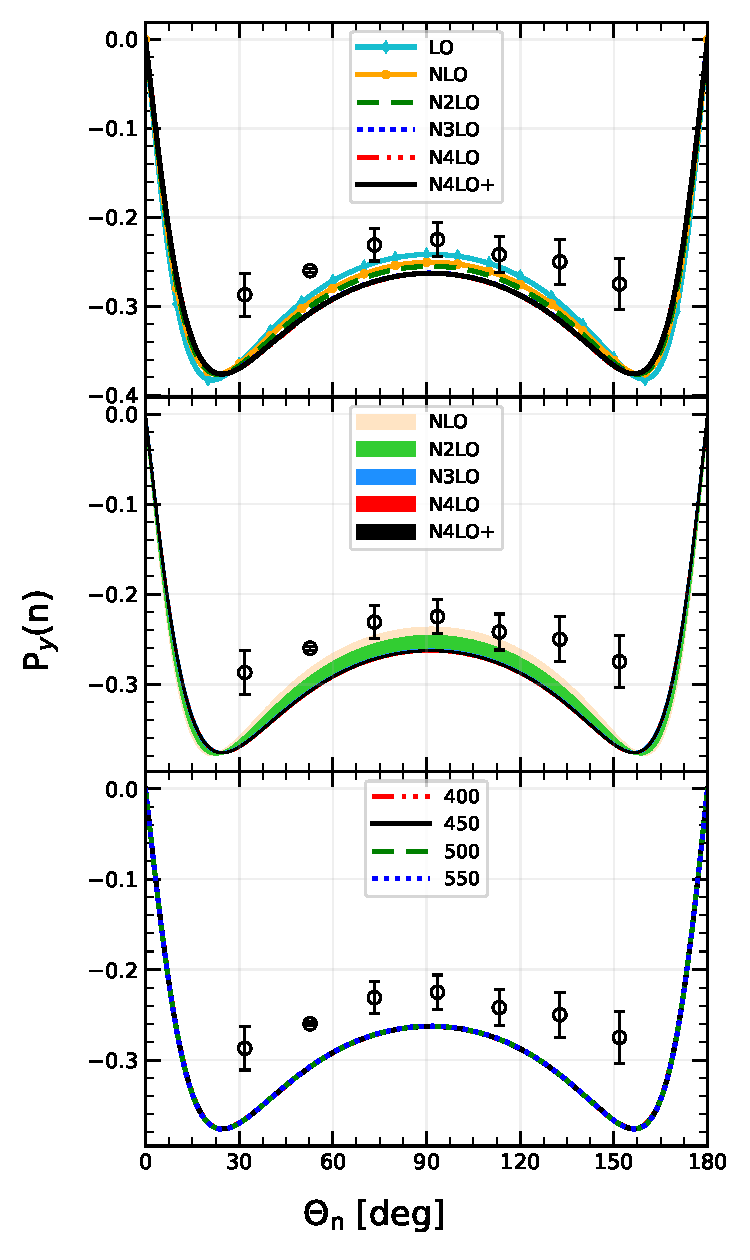
\includegraphics[width=\textwidth]{Figures_De/POLNOUT2(y)_2.75mev_neuteron.pdf}
            \label{Pn_2p75_vert}
        \end{subfigure}
        \begin{subfigure}[b]{0.46\textwidth}
            \caption{\small E$_\gamma = 100$~MeV}
            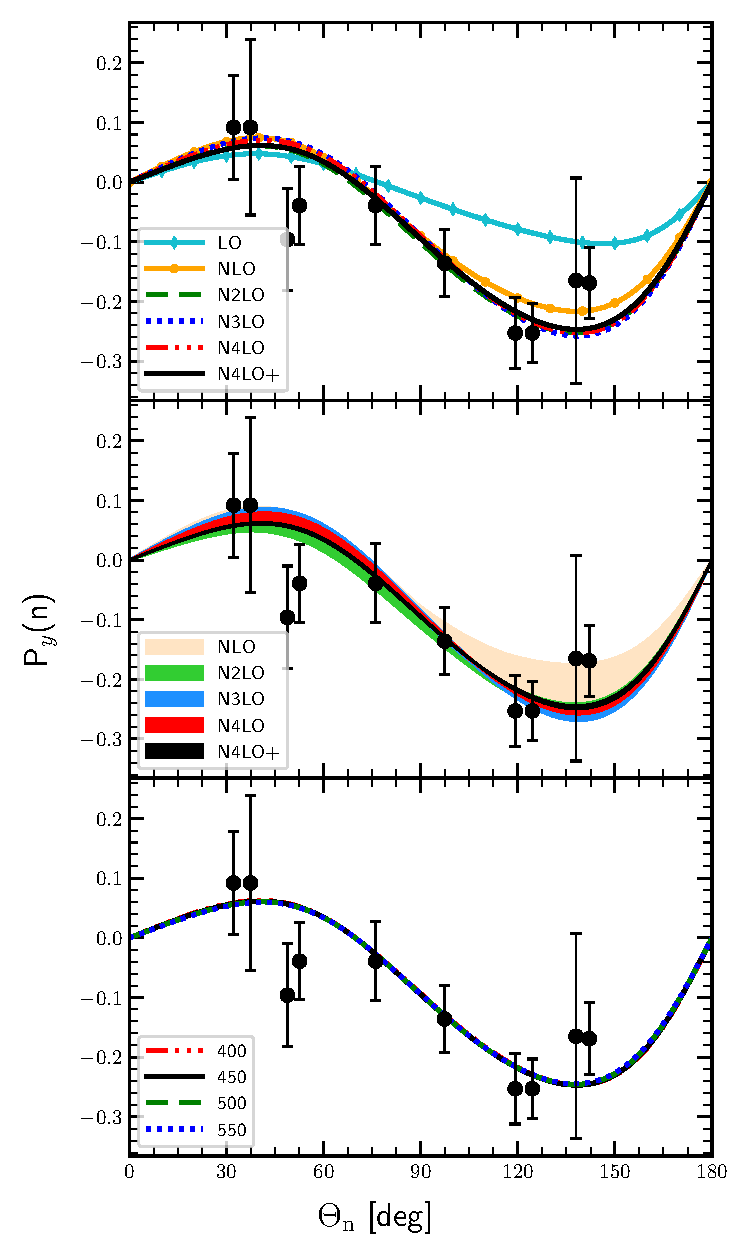
\includegraphics[width=\textwidth]{Figures_De/POLNOUT2(y)_100mev_neuteron.pdf}
            \label{Pn_100_vert}
        \end{subfigure}
        \caption{The same as in \fig{PY_30_100_vert} but for the neutron polarization
        $P_y(n)$ and at photon energies \SI{2.75}{\mev} {\bf (a)} and \SI{100}{\mev} {\bf (b)}.
        Data are from \cite{Jewell_neuteronpolarization} (empty circles)
        and \cite{CAMERON_neuteronpolarization} (filled circles).}
        \label{Pn_2p75_100}
    \end{figure}


\clearpage

\section{Helium-3 photodisintegration}
\label{sec:hel_results}

\subsection{Three-body breakup}
\label{sec:hel_3N}

    In this section I will discuss results
    for $^3\text{He} \rightarrow p + p + n$ process differential
    cross-section obtained with \tmp{???} model of nuclear current.
    For three free nuclepns in the final state it is convenient to
    introduce, as a kinematical variable, the arc-length of the S-curve.
    For giving direction of two momenta $\hat{p}_1$ and $\hat{p}_2$,
    the S-curve spans in the plane defined by kinetic energies of the 
    same two nucleons, $E_1$ and $E_2$.

    For three particles and known initial energy and momenta five kinematical
    variables\footnote{Among nine variables describing final state 
    $\vec{p}_1,\vec{p}_2$ and $\vec{p}_3$, four can be derived from 
    energy and momentum conservation laws.}
    are required to define the final kinematics.
    We choose four variables as directions of outgoing nucleons no 1 and 2:
    $\theta_1, \phi_1, \theta_2$ and $\phi_2$, with the $z$-axis aligned to the 
    photon momentum. Choosing $E_1$ as the fiveth variable would introduce
    ambiguity, as in some cases two values of $E_2$ could be allowed.
    Instead, the location on the S-curve defines the kinematical configuration
    unambiguousely.
    The various possible locations of the S-curve in $E_1-E_2$ plane,
    as well as the convention on choosing the $S=0$ point in given
    in Fig.~1 of \cite{GLOCKLE_report_1996}.
    
    In the \fig{CROSS_HE_EXCL_30} I demonstrate a differential cross section 
    $\frac{d^5\sigma}{d\Omega_1d\Omega_2dS}$ as a function of the S arc length
    and as in previous section, I study the convergence with respect to chiral
    order and the cut-off dependance.
    The photon energy is  E$_\gamma=\SI{30}{\mev}$; the kinematic configuration
    $\theta_1 = \ang{15}$, $\phi_1 = \ang{0}$,
    $\theta_2 = \ang{15}$, $\phi_2 = \ang{180}$ and predictions have been
    obtained without 3NF.\footnote{Different kinematic configurations $\theta_1$, $\phi_1$,
    $\theta_2$ and $\phi_2$ have been tested with a step of \ang{15}
    and most interesting cases(showing largest descripancies) are presented in this work.}
    On the left we see that only \gls{nlo} and \gls{n2lo} introduce relatively large truncation error.
    The maximal width of a band for NLO is \SI{37.6}{\percent} at $S=\SI{10}{\mev}$,
    for \gls{n2lo} it is \SI{12.4}{\percent} at the same S-value and it is gradually decreasing
    coming to \SI{0.13}{\percent} at \gls{n4lo+}.
    The cut-off spread(right) is bigger around maxima values but remains below
    \SI{3}{\percent}. It reaches
    \SI{0.78}{\percent} at the minimum point ($S=\SI{10}{\mev}$).
    

    \begin{figure}[h]
        \begin{center}
            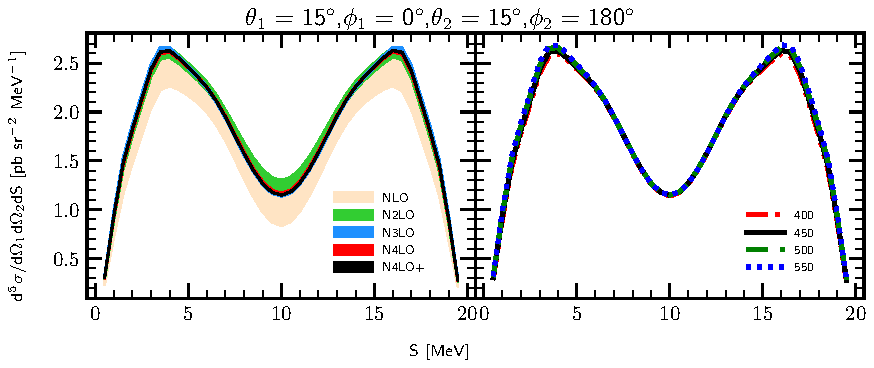
\includegraphics[width=0.9\textwidth]{Figures_HE/CROSS_excl_trunc_30mev.pdf}
            \end{center}
            \caption{The five-fold differential cross section for the photon 
            energy E$_\gamma=\SI{30}{\mev}$ for the kinematic configuration
            $\theta_1 = \ang{15}$, $\phi_1 = \ang{0}$,
            $\theta_2 = \ang{15}$, $\phi_2 = \ang{180}$.
            The left figure presents truncation error bands obtained using the \gls{sms} potential
            with chiral orders from \gls{nlo} to \gls{n4lo+}, and with
            cut-off parameter $\Lambda=\SI{450}{\mev}$.
            The right figure presents a cut-off dependence at \gls{n4lo+}.
            Results are obtained with two-nucleon force only and \gls{snc} current
            and Siegert theorem used for a 2NC contributions.}
            \label{CROSS_HE_EXCL_30}
        \end{figure}

    With larger energy E$_\gamma=\SI{100}{\mev}$, for which predictions
    are demonstrated in the \fig{CROSS_HE_EXCL_100},
    both truncation error and cut-off spread become larger.
    The truncation band at the maximum point at $S=\SI{10}{\mev}$ for NLO is \SI{55.0}{\percent}
    decreasing to \SI{2.2}{\percent} at \gls{n4lo+} which still is around 3 times larger than
    it was for predictions at E$_\gamma=\SI{30}{\mev}$.
    The cut-off spread also becomes larger with increasing energy value: \SI{9.0}{\percent}
    at the same (maximum) point which is also $\sim 3$ times bigger than the one we observed
    for the lower energy.

        \begin{figure}[h]
            \begin{center}
            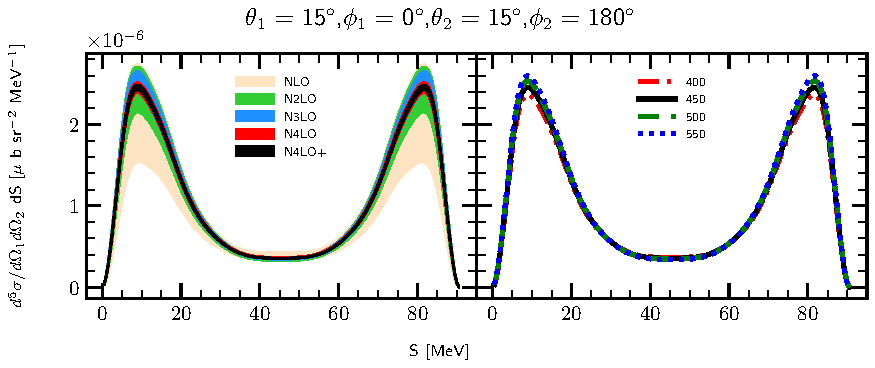
\includegraphics[width=0.9\textwidth]{Figures_HE/CROSS_excl_trunc_100mev.pdf}
            \end{center}
            \caption{The same as in \fig{CROSS_HE_EXCL_30} but 
            for the photon energy E$_\gamma=100$~MeV}
            \label{CROSS_HE_EXCL_100}
        \end{figure}

    Results for the same E$_\gamma=100$~MeV but other angular configuration  
    $\theta_1 = \ang{75}$, $\phi_1 = \ang{75}$,
    $\theta_2 = \ang{75}$, $\phi_2 = \ang{105}$ are
    given in \fig{CROSS_HE_EXCL_75_75_75_105}.
    The top row shows results obtained with 2NF only, while predictions obtained with 3NF are shown
    on the bottom row.
    It seems that 3NF does not change much the convergence with respect to the chiral order:
    truncation error band at the point of maximum $S=\SI{35}{\mev}$ (\gls{n4lo+})
    is \SI{1.11}{\percent} and \SI{1.16}{\percent} with and without 3NF, respectively.
    As it is almost the same, I conclude that inclusion \gls{n2lo} 3NF practically
    does not affect chiral order convergence.
    Note, 3NF at \gls{n2lo} has been used for all forces above \gls{nlo}.

    The cut-off dependence, in turn, is affected by the presence of 3NF. Predictions with 2NF only have
    \SI{13.7}{\percent} spread at the same maximum point $S=\SI{35}{\mev}$, while predictions with 3NF
    have only \SI{1.23}{\percent} relative spread, so the difference is tremendous.

        \begin{figure}[h]
            \begin{center}
                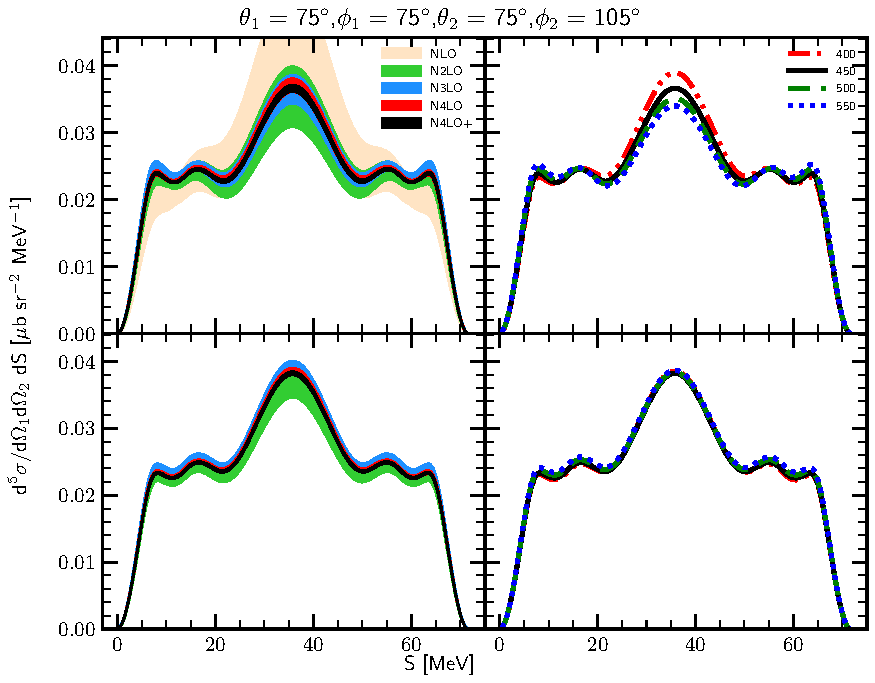
\includegraphics[width=0.9\textwidth]{Figures_HE/CROSS_excl_trunc_100mev_75_75_75_105_2NF_3NF.pdf}
                \end{center}
                \caption{The same as in the \fig{CROSS_HE_EXCL_100} but for the kinematic
                configuration at
                $\theta_1 = \ang{75}$, $\phi_1 = \ang{75}$,
                $\theta_2 = \ang{75}$ and $\phi_2 = \ang{105}$.
                Results obtained with the chiral \gls{sms} 2N force 
                are presented on the top row. The same, but
                with the \gls{n2lo} 3NF included is presented on the bottom row
                (starting from the \gls{n2lo} - where 3NF appears for the first time).}
                \label{CROSS_HE_EXCL_75_75_75_105}
        \end{figure}


    Similar trends are present also in other configurations, demonstrated for the comparison:
    Figs.\ref{CROSS_HE_EXCL_15_105_15_75},
    Figs.\ref{CROSS_HE_EXCL_45_75_45_105} and
    Figs.\ref{CROSS_HE_EXCL_165_15_15_165}.

    
        \begin{figure}[h]
            \begin{center}
                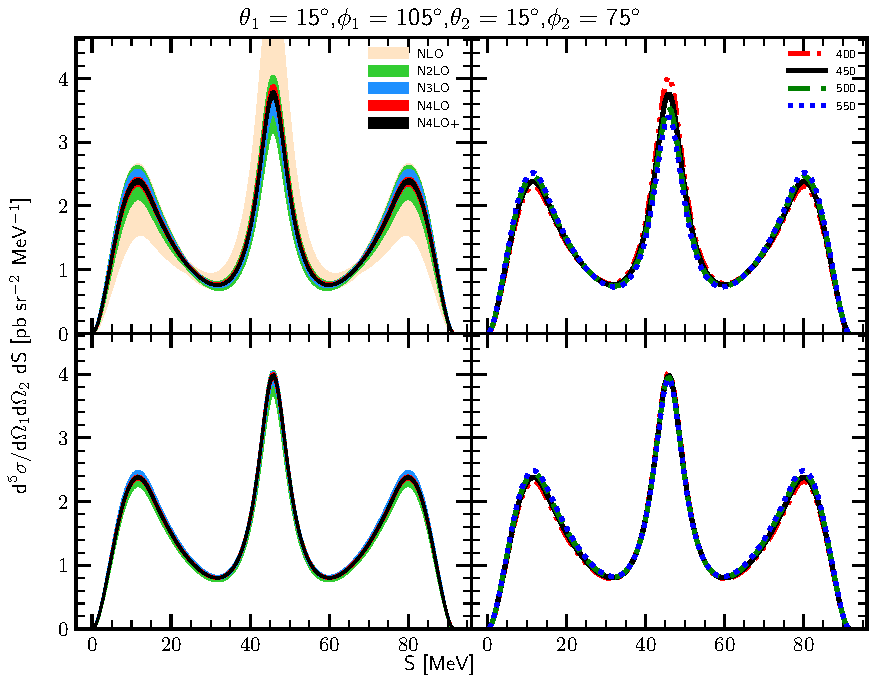
\includegraphics[width=0.9\textwidth]{Figures_HE/CROSS_excl_trunc_100mev_15_105_15_75_2NF_3NF.pdf}
                \end{center}
                \caption{The same as in the \fig{CROSS_HE_EXCL_75_75_75_105} but for the kinematic
                configuration at
                $\theta_1 = \ang{15}$, $\phi_1 = \ang{105}$,
                $\theta_2 = \ang{15}$ and $\phi_2 = \ang{75}$.}
                \label{CROSS_HE_EXCL_15_105_15_75}
        \end{figure}




        \begin{figure}[h]
            \begin{center}
                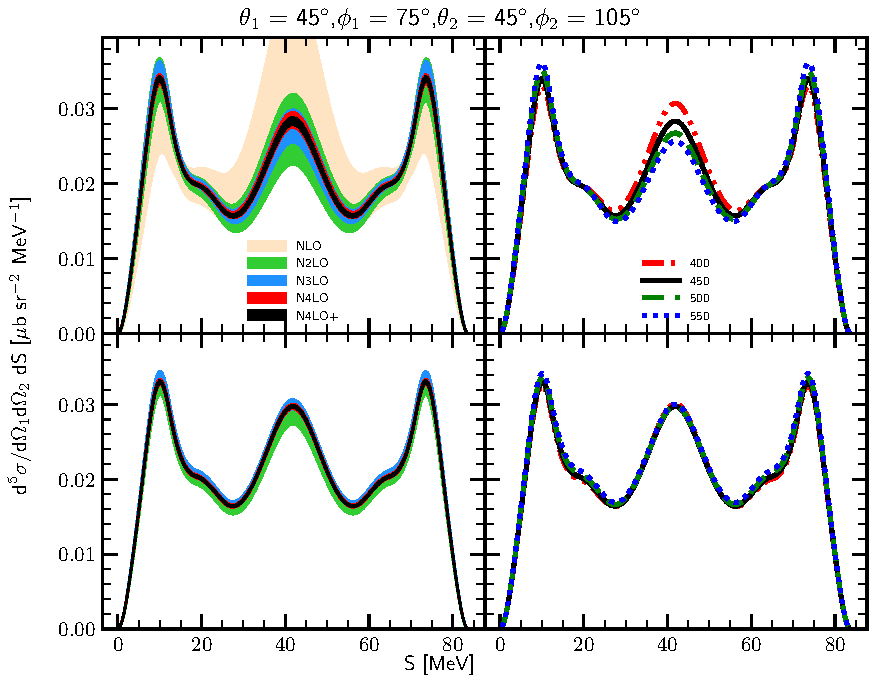
\includegraphics[width=0.9\textwidth]{Figures_HE/CROSS_excl_trunc_100mev_45_75_45_105_2NF_3NF.pdf}
                \end{center}
                \caption{The same as in the \fig{CROSS_HE_EXCL_15_105_15_75} but for the different kinematic
                configuration.}
                \label{CROSS_HE_EXCL_45_75_45_105}
        \end{figure}


        \begin{figure}[h]
            \begin{center}
                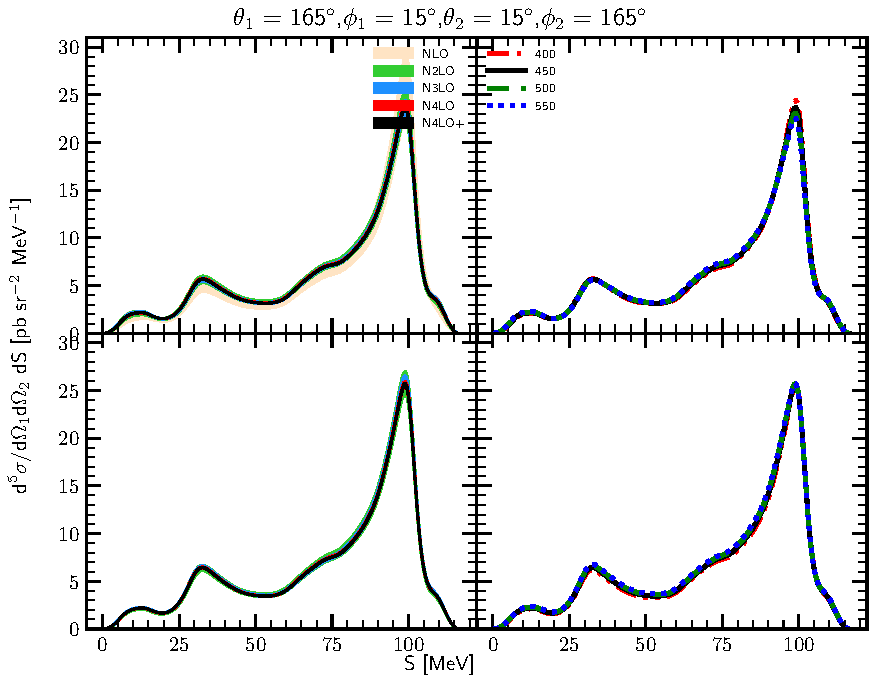
\includegraphics[width=0.9\textwidth]{Figures_HE/CROSS_excl_trunc_100mev_165_15_15_165_2NF_3NF.pdf}
                \end{center}
                \caption{The same as in the \fig{CROSS_HE_EXCL_45_75_45_105} but for the kinematic
                configuration at
                $\theta_1 = \ang{165}$, $\phi_1 = \ang{15}$,
                $\theta_2 = \ang{15}$ and $\phi_2 = \ang{165}$.}
                \label{CROSS_HE_EXCL_165_15_15_165}
        \end{figure}


        The exclusive cross-sections shown above, in Figs.~\ref{CROSS_HE_EXCL_30}-\ref{CROSS_HE_EXCL_165_15_15_165}
        are small and unfortunately below the possibilities of current 
        experimental techniques. The semi-inclusive measurement is more likely to be
        performed, thus in Figs \ref{CROSS_HE_INCL_30MEV_2NF} and \ref{CROSS_HE_INCL_100MEV_2NF}
        I show the 
        differential cross section $\frac{d^3\sigma}{d\Omega_p d\text{E}_p}$.
        I choose the same photon energies as above: E$_\gamma = \SI{30}{\mev}$ and
        E$_\gamma = \SI{100}{\mev}$.
        Each figure consists of subfigures where each row presents results
        for a proton momenta polar angle $\theta_p = \ang{10}, \ang{50}, \ang{90}, \ang{130}$ and \ang{170}.
        The left part of each subfigure shows detected
        chiral order dependence while the right - the cut-off dependence.
        
        At the photon energy \SI{30}{\mev} the chiral dependence is relatively weak: at the maximum point
        ($E_p \simeq \SI{3.8}{\mev}$) the relative difference varies between \SI{12}{\percent} and 
        \SI{28}{\percent} at LO for different angles. This difference decreases with each subsequent order
        resulting in maximum \SI{0.15}{\percent} at $N^4LO+$. At the energy $\text{E}_\gamma = \SI{100}{\mev}$ truncation errors
        are larger: at the maximum around $E_p \simeq \SI{1.46}{\mev}$ the discrepancy is around \SI{40}{\percent} (NLO),
        \SI{15}{\percent} (N2LO), coming to \SI{1.5}{\percent} at \gls{n4lo+}.

        A typical cut-off uncertainty at $\text{E}_\gamma = \SI{30}{\mev}$ is around \SI{2}{\percent}
        and at $\text{E}_\gamma = \SI{100}{\mev}$ increases up to \SI{8}{\percent} for all angles and 
        at the same values of $E_p$ as regarded above.

        Observed small uncertainties allow me to conclude that the semi-inclusive cross-section
        $\frac{d^3\sigma}{d\Omega_p d\text{E}_p}$ is not useful in studies aiming on
        pin-down the details of the chiral force.
        \tmp{do we have prediction with othe current?}  



        \begin{figure}[h]
            \begin{center}
            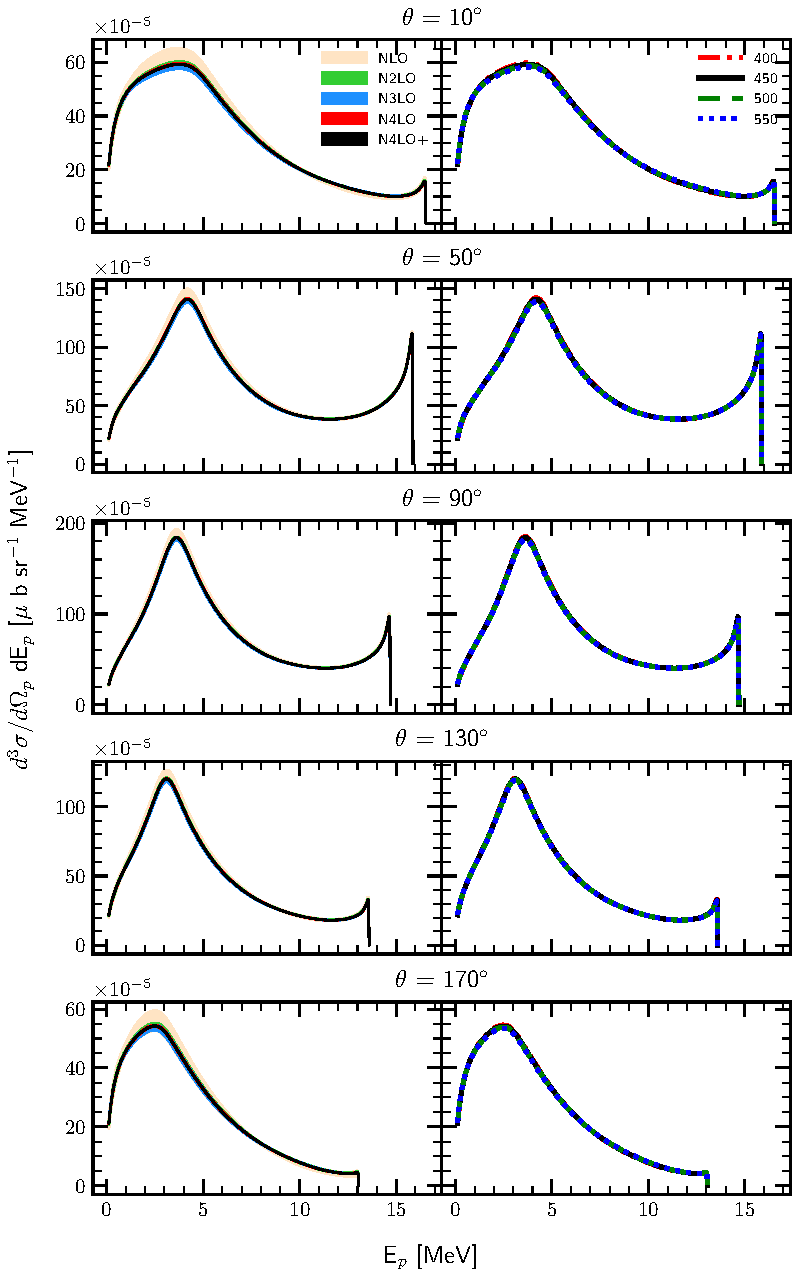
\includegraphics[width=0.8\textwidth]{Figures_HE/CROSS_incl_trunc_30mev_all.pdf}
            \end{center}
            \caption{The semi-inclusive differential cross section $\frac{d^3\sigma}{d\Omega_p d\text{E}_p}$
            at E$_\gamma = \SI{30}{\mev}$ $\phi_1 = \ang{0}$ as a function of outgoing proton energy E$_p$. Each row represents 
            predictions for different values of the outgoing proton's momentum polar angle $\theta_p$: 
            \ang{10}, \ang{50}, \ang{90}, \ang{130} and \ang{170}.
            The left figure presents truncation error bands obtained using the \gls{sms} potential
            with chiral orders from \gls{nlo} to \gls{n4lo+}, and with
            cut-off parameter $\Lambda=\SI{450}{\mev}$.
            The right figure presents a cut-off dependence at \gls{n4lo+}.
            Predictions have been obtained with the \gls{sms} NN potential but neglecting 3NF.}
            \label{CROSS_HE_INCL_30MEV_2NF}
        \end{figure}

        \begin{figure}[h]
            \begin{center}
            \includegraphics[width=0.8\textwidth]{Figures_HE/CROSS_incl_trunc_100mev_all.pdf}
            \end{center}
            \caption{The same as in \fig{CROSS_HE_INCL_30MEV_2NF} but for E$_\gamma = \SI{100}{\mev}$.
            \tmp{stylisticchages: axis label shift to left, change units to pb}}
            \label{CROSS_HE_INCL_100MEV_2NF}
        \end{figure}


\clearpage


\subsection{Two-body breakup}

    The differential cross section $d\sigma/d\Omega_d$ for the $^3\text{He} + \gamma \rightarrow d + p$ reaction
    is presented In the \fig{CROSS_nd_30} (for the photon energy $\text{E}_\gamma = \SI{30}{\mev}$)
    and In the \fig{CROSS_nd_100} (for the photon energy $\text{E}_\gamma = \SI{100}{\mev}$).
    We see that both truncation and cut-off uncertainties are larger with increasing photon energy.
    The relative spread of the truncation error at the maximum point ($\theta_p = \ang{105}$)
    for the lower energy is \SI{0.05}{\percent} at \gls{n4lo+}, while for the larger energy
    similar spread is \SI{0.45}{\percent} (at \gls{n4lo+}, $\theta_p = \ang{120}$).

    The cut-off dependence is also stronger for the larger energy:
    it is  \SI{1.45}{\percent} at \SI{30}{\mev} and \SI{4.01}{\percent} at \SI{100}{\mev}
    (at the points of maximum). 

\begin{figure}[h]
    \begin{center}
        \includegraphics[width=0.9\textwidth]{Figures_HE/CROSS_nd_trunc_30mev.pdf}
        \end{center}
        \caption{Differential cross section for the D-$p$ 
        two-body photodisintegraion of $^3$He as a function of the d$\gamma$ angle.
        The initial photon energy $\text{E}_\gamma=\SI{30}{\mev}$.}
        \label{CROSS_nd_30}
    \end{figure}


    \begin{figure}[h]
        \begin{center}
        \includegraphics[width=0.9\textwidth]{Figures_HE/CROSS_nd_trunc_100mev.pdf}
        \end{center}
        \caption{The same as on \fig{CROSS_nd_30} but 
        for the photon energy E$_\gamma=\SI{100}{\mev}$}
        \label{CROSS_nd_100}
    \end{figure}

    \clearpage
\section{Triton photodisintegration}
    \label{sec:triton_results}
    
    
    In this section I will discuss results
    for $^3\text{H} \rightarrow p + n + n$ process.

    In the \fig{CROSS_Triton_EXCL_30_15_0_15_180} I demonstrate a differential cross section 
    $\frac{d^5\sigma}{d\Omega_1d\Omega_2dS}$ as a function of the S arc length.
    The photon energy is  E$_\gamma=\SI{30}{\mev}$ and the kinematic configuration
    $\theta_1 = \ang{15}$, $\phi_1 = \ang{0}$,
    $\theta_2 = \ang{15}$, $\phi_2 = \ang{180}$; predictions have been obtained without 3NF.
    We see that only \gls{nlo} and \gls{n2lo} introduce relatively large truncation error.
    The maximal width of a band for NLO is \SI{30.95}{\percent} at $S=\SI{10}{\mev}$,
    for \gls{n2lo} it is \SI{6.79}{\percent} at the same point and it is gradually decreasing
    coming to \SI{0.10}{\percent} at \gls{n4lo+}.
    The cut-off spread around maxima values is \SI{6.25}{\percent} (at $S=\SI{4}{\mev}$) and it is
    \SI{1.81}{\percent} at $S=\SI{10}{\mev}$.

    \begin{figure}[h]
        \begin{center}
            \includegraphics[width=0.9\textwidth]{Figures_Triton/CROSS_excl_trunc_30mev_15_0_15_180_2NF.pdf}
            \end{center}
            \caption{The five-fold differential cross section for the photon 
            energy E$_\gamma=\SI{30}{\mev}$ for the kinematic configuration
            $\theta_1 = \ang{15}$, $\phi_1 = \ang{0}$,
            $\theta_2 = \ang{15}$, $\phi_2 = \ang{180}$.
            The left figure presents truncation error bands obtained using potential
            with chiral orders from \gls{nlo} to \gls{n4lo+}, and with
            cut-off parameter $\Lambda=\SI{450}{\mev}$.
            The right figure presents a cut-off dependence at \gls{n4lo+}.
            Results are obtained with two-nucleon force only.}
            \label{CROSS_Triton_EXCL_30_15_0_15_180}
    \end{figure}

    With larger energy E$_\gamma=\SI{100}{\mev}$ demonstrated in the \fig{CROSS_Triton_EXCL_100mev_15_0_15_180},
    the truncation band at the maximum point $S=\SI{10}{\mev}$ for NLO is \SI{50.26}{\percent}
    decreasing to \SI{2.00}{\percent} at \gls{n4lo+}.
    The cut-off spread also becomes larger with increasing energy value: \SI{9.52}{\percent}
    at the same (maximum).

    The truncation error bands and cut-off dependance is very similar as it was for
    the three-body Helium photodisintegration \ref{sec:hel_3N} and the relative errors 
    have a similar range of values.

    \begin{figure}[h]
        \begin{center}
            \includegraphics[width=0.9\textwidth]{Figures_Triton/CROSS_excl_trunc_100mev_15_0_15_180_2NF.pdf}
            \end{center}
            \caption{The same as in the \fig{CROSS_Triton_EXCL_30_15_0_15_180} but for the photon energy
            E$_\gamma = \SI{100}{\mev}$.}
            \label{CROSS_Triton_EXCL_100mev_15_0_15_180}
    \end{figure}



    Results for other angular configurations at 
    $\theta_1 = \ang{75}$, $\phi_1 = \ang{75}$,
    $\theta_2 = \ang{75}$, $\phi_2 = \ang{105}$ are
    demonstrated in \fig{CROSS_Triton_EXCL_75_75_75_105} with E$_\gamma=\SI{30}{\mev}$.
    Both truncation errors and cut-off dependance are lower at this configuration:
    the relative  width of the truncation band at \gls{nlo} is \SI{9.39}{\percent}
    (at the maximum point $S=\SI{8}{\mev}$) and drops to only \SI{0.1}{\percent}
    at \gls{n4lo+}. The relative cut-off spread is \SI{0.93}{\percent} at the same point.

    At the larger energy E$_\gamma=\SI{100}{\mev}$ demonstrated in \fig{CROSS_Triton_EXCL_100mev_75_75_75_105}
    uncertainties have been increased. The truncation bands are \SI{44.42}{\percent} and 
    \SI{2.09}{\percent} (at \gls{nlo} and \gls{n4lo+} respectively) and
    the cut-off spread is \SI{13.04}{\percent} (all at $S=\SI{35}{\mev}$).


    \begin{figure}[h]
        \begin{center}
            \includegraphics[width=0.9\textwidth]{Figures_Triton/CROSS_excl_trunc_30mev_75_75_75_105_2NF.pdf}
            \end{center}
            \caption{The same as in the \fig{CROSS_Triton_EXCL_30_15_0_15_180} but for the different kinematic
            configuration
            $\theta_1 = \ang{75}$, $\phi_1 = \ang{75}$,
            $\theta_2 = \ang{75}$, $\phi_2 = \ang{105}$.
            Results obtained with 2NF only.}
            \label{CROSS_Triton_EXCL_75_75_75_105}
    \end{figure}


    \begin{figure}[h]
        \begin{center}
            \includegraphics[width=0.9\textwidth]{Figures_Triton/CROSS_excl_trunc_100mev_75_75_75_105_2NF.pdf}
            \end{center}
            \caption{The same as in the \fig{CROSS_Triton_EXCL_75_75_75_105} but for the photon energy
            E$_\gamma = \SI{100}{\mev}$.}
            \label{CROSS_Triton_EXCL_100mev_75_75_75_105}
    \end{figure}

    Similar trends are present also in other configurations, demonstrated for the comparison:
    Figs.~\ref{CROSS_Triton_EXCL_15_105_15_75},
    \ref{CROSS_Triton_EXCL_100mev_15_105_15_75},
    \ref{CROSS_Triton_EXCL_45_75_45_105},
    \ref{CROSS_Triton_EXCL_100mev_45_75_45_105},
    \ref{CROSS_Triton_EXCL_165_15_15_165}
    and
    \ref{CROSS_Triton_EXCL_100mev_165_15_15_165}.

    \begin{figure}[h]
        \begin{center}
            \includegraphics[width=0.9\textwidth]{Figures_Triton/CROSS_excl_trunc_30mev_15_105_15_75_2NF.pdf}
            \end{center}
            \caption{The same as in the \fig{CROSS_Triton_EXCL_75_75_75_105} but for the different kinematic
            configuration
            $\theta_1 = \ang{15}$, $\phi_1 = \ang{105}$,
            $\theta_2 = \ang{15}$, $\phi_2 = \ang{75}$.
            Results obtained with 2NF only.}
            \label{CROSS_Triton_EXCL_15_105_15_75}
    \end{figure}


    \begin{figure}[h]
        \begin{center}
            \includegraphics[width=0.9\textwidth]{Figures_Triton/CROSS_excl_trunc_100mev_15_105_15_75_2NF.pdf}
            \end{center}
            \caption{The same as in the \fig{CROSS_Triton_EXCL_15_105_15_75} but for the photon energy
            E$_\gamma = \SI{100}{\mev}$.}
            \label{CROSS_Triton_EXCL_100mev_15_105_15_75}
    \end{figure}

    \begin{figure}[h]
        \begin{center}
            \includegraphics[width=0.9\textwidth]{Figures_Triton/CROSS_excl_trunc_30mev_45_75_45_105_2NF.pdf}
            \end{center}
            \caption{The same as in the \fig{CROSS_Triton_EXCL_15_105_15_75} but for the different kinematic
            configuration
            $\theta_1 = \ang{45}$, $\phi_1 = \ang{75}$,
            $\theta_2 = \ang{45}$, $\phi_2 = \ang{105}$.
            Results obtained with 2NF only.}
            \label{CROSS_Triton_EXCL_45_75_45_105}
    \end{figure}


    \begin{figure}[h]
        \begin{center}
            \includegraphics[width=0.9\textwidth]{Figures_Triton/CROSS_excl_trunc_100mev_45_75_45_105_2NF.pdf}
            \end{center}
            \caption{The same as in the \fig{CROSS_Triton_EXCL_45_75_45_105} but for the photon energy
            E$_\gamma = \SI{100}{\mev}$.}
            \label{CROSS_Triton_EXCL_100mev_45_75_45_105}
    \end{figure}

    \begin{figure}[h]
        \begin{center}
            \includegraphics[width=0.9\textwidth]{Figures_Triton/CROSS_excl_trunc_30mev_165_15_15_165_2NF.pdf}
            \end{center}
            \caption{The same as in the \fig{CROSS_Triton_EXCL_45_75_45_105} but for the different kinematic
            configuration
            $\theta_1 = \ang{165}$, $\phi_1 = \ang{15}$,
            $\theta_2 = \ang{15}$, $\phi_2 = \ang{165}$.
            Results obtained with 2NF only.}
            \label{CROSS_Triton_EXCL_165_15_15_165}
    \end{figure}


    \begin{figure}[h]
        \begin{center}
            \includegraphics[width=0.9\textwidth]{Figures_Triton/CROSS_excl_trunc_100mev_165_15_15_165_2NF.pdf}
            \end{center}
            \caption{The same as in the \fig{CROSS_Triton_EXCL_165_15_15_165} but for the photon energy
            E$_\gamma = \SI{100}{\mev}$.}
            \label{CROSS_Triton_EXCL_100mev_165_15_15_165}
    \end{figure}
        
        
    \clearpage
\section{Pion absorption from the lowest atomic orbital}
\label{sec:pion_results}

\subsection{Pion absorption in $^2$H}

    \begin{figure}[h]
        \begin{center}
        \includegraphics[width=0.6\textwidth]{PlotData/PION/Dalitz_maps/figures/Gamma_nn.pdf}
        \end{center}
        \caption{
            Absorption rate for the reaction $\pi^- + {^2{\rm H}} \rightarrow n + n$.
            The rates were calculated using the \gls{sms} force with different chiral orders and cut-off values.
            The results were obtained using the single-nucleon transition operator and 
            including two-nucleon contributions at the leading order.
            The figure shows the results obtained using plane wave (PW) plus
            two-neutron rescattering (Full) parts.
            The experimental value is obtained from the hadronic
            ground-state broadening in pionic deuterium~\cite{Strauch2010,Strauch2011}.}
        \label{Gamma_nn}
    \end{figure}


    \subsection{Pion absorption in $^3$He}

    in \fig{Gamma_pnn} and \ref{Gamma_nd} the pion absorption rates are presented as a function
    of the chiral order with different values of the cut-off parameter
    (for $\pi^- + ^3\text{He} \rightarrow p + n + n$ and $\pi^- + ^3\text{He} \rightarrow n + d$ reactions, respectively).
    Both figures show that with fixed chiral order the arrangement of values with respect of the cut-off parameter
    remains the same, namely with increasing $\Lambda$, absorption rate decreases. The only exception in both cases 
    appears at \gls{n3lo} where prediction with $\Lambda = \SI{550}{\mev}$ goes above other predictions.
    At the next order, \gls{n4lo}, it corrects to the normal arrangement.
    This behavior may be connected to the 3NF used for the calculation and in order to check that I show
    a similar figure for a proton radius $r_p$ in \fig{proton_rad} calculated with 
    and without 3NF (left and right panels respectively). Results obtained with 3NF show
    similar deviation at \gls{n3lo} while data obtained without 3NF does not have that.
    Nevertheless, the spread of predictions with respect to the cut-off values is much smaller
    with 3NF and deviation seems to be not crucial as total difference
    between predictions in this case is very small.




    \begin{figure}[h]
        \begin{center}
        \includegraphics[width=0.6\textwidth]{PlotData/PION/Dalitz_maps/figures/Gamma_pnn.pdf}
        \end{center}
        \caption{Absorption rate for $\pi^- + ^3\text{He} \rightarrow p + n + n$ reaction as a function
        of the chiral order with different values of the cut-off parameter $\Lambda$.
        Predictions were obtained with 3NF.}
        \label{Gamma_pnn}
    \end{figure}

    \begin{figure}[h]
        \begin{center}
        \includegraphics[width=0.6\textwidth]{PlotData/PION/Dalitz_maps/figures/Gamma_nd.pdf}
        \end{center}
        \caption{The same as in \fig{Gamma_pnn}, but for $\pi^- + ^3\text{He} \rightarrow n + d$ reaction.}
        \label{Gamma_nd}
    \end{figure}

    \begin{figure}[h]
        \begin{center}
        \includegraphics[width=0.99\textwidth]{PlotData/PION/Dalitz_maps/figures/proton_radius_mt31_3NF.pdf}
        \end{center}
        \caption{\tmp{check mt3} Proton radius $r_p$ as a function of the chiral order calculated with
        different values of the cut-off parameter $\Lambda$. The radius was calculated with 2NF and 3NF (left panel)
        and with 2NF only (right panel).}
        \label{proton_rad}
    \end{figure}

    In Figs.~\ref{pion_map_E1E2_cutoff} and \ref{pion_map_xy_cutoff} I show 
    intensity plots for the double differential absorption rates
    $d^2 \Gamma_{pnn}/dE_1dE_2$ for the $\pi^- + ^3\text{He} \rightarrow p + n + n$
    process as functions of the nucleons energies (nucleon number 1 is a proton) and 
    of Dalitz coordinates ($x$ and $y$), respectively.

    In \fig{pion_map_xy_cutoff} coordinates $x$ and $y$ are defined as:

    \begin{align}
        x &= 3 (E_1 + 2E_2 - E)/E, \nonumber\\
        y &= (3E_1 - E)/E,
        \label{dalitz_xy}
    \end{align}
    taking the region where $r^2 \equiv x^2 + y^2 \leq 1$.

    Each of two figures consists of four panels representing predictions obtained with different 
    values of the cut-off parameter $\Lambda$. The difference between predictions which can be 
    noticed with the naked eye - is that area of the central region (corresponding to smallest values)
    becomes larger with increasing $\Lambda$. It coheres to what we saw in \fig{Gamma_pnn}
    where total absorption rate was inversely correlated with cut-off parameter. The dominant contribution
    comes from the region with lowest proton energy values of $E_1 \rightarrow 0$ where both neutrons have similar large values.
    This is a situation when proton is a spectator while both neutrons share all energy
    - quasi-free scattering(QFS). 

    Another region with high absorption rate is neutron-neutron final state interaction (FSI(nn)).
    It is located at high $E_1$ when proton gets one third part of total energy while neutrons both get
    one sixth.
    
        \begin{figure}[h]
            \begin{center}
            \includegraphics[width=0.7\textwidth]{PlotData/PION/Dalitz_maps/figures/Dalitz_map_pnn_E1E2_cutofs.pdf}
            \end{center}
            \caption{Intensity plots for the double differential absorption rates
            $d^2 \Gamma_{pnn}/dE_1dE_2$ for the $\pi^- + ^3\text{He} \rightarrow p + n + n$
            process, obtained using the SMS potential at \gls{n4lo+}
            with all contributions possible: plane wave + rescattering, 1NC + 2N, 2NF+3NF.
            Each panel present predictions obtained with different values of the cut-off parameter $\Lambda$:
            from \SI{400}{\mev} (upper left) to \SI{550}{\mev} (lower right). Nucleon 1 is a proton.}
            \label{pion_map_E1E2_cutoff}
        \end{figure}

    \begin{figure}[h]
        \begin{center}
        \includegraphics[width=0.7\textwidth]{PlotData/PION/Dalitz_maps/figures/Dalitz_map_pnn_xy_cutofs.pdf}
        \end{center}
        \caption{The same as in \fig{pion_map_E1E2_cutoff} but for the double differential absorption rates
        $d^2 \Gamma_{pnn}/dxdy$.}
        \label{pion_map_xy_cutoff}
    \end{figure}

    Next I show similar colormaps but for the predictions obtained with plane wave component only (without rescattering part)
    in Figs.~\ref{pion_map_E1E2_cutoff_PW} and \ref{pion_map_xy_cutoff_PW}. Presented plots show that
    the difference of predictions obtained without rescattering part with full is very large. 
    Predicted values 
    are few times larger and the distribution is completely different.
    The FSI(nn) region is not presented here in a sense that there is no peak with respect to other 
    values. The QFS region is, on the contrary, 
    which obviously tells us that one has to take into account rescattering pat in order to obtain relevant results.   

    \begin{figure}[h]
        \begin{center}
        \includegraphics[width=0.7\textwidth]{PlotData/PION/Dalitz_maps/figures/Dalitz_map_pnn_E1E2_cutofs_PWIAS.pdf}
        \end{center}
        \caption{Intensity plots for the double differential absorption rates
        $d^2 \Gamma_{pnn}/dE_1dE_2$ for the $\pi^- + ^3\text{He} \rightarrow p + n + n$
        process, obtained using the SMS potential at \gls{n4lo+}
        with plane wave part only (without rescattering).
        All other contributions are the same as in \fig{pion_map_E1E2_cutoff}: 1NC + 2N and 2NF+3NF.
        Each panel present predictions obtained with different values of the cut-off parameter $\Lambda$:
        from \SI{400}{\mev} (upper left) to \SI{550}{\mev} (lower right). Nucleon 1 is a proton.}
        \label{pion_map_E1E2_cutoff_PW}
    \end{figure}

    \begin{figure}[h]
        \begin{center}
        \includegraphics[width=0.7\textwidth]{PlotData/PION/Dalitz_maps/figures/Dalitz_map_pnn_xy_cutofs_PWIAS.pdf}
        \end{center}
        \caption{The same as in \fig{pion_map_E1E2_cutoff_PW} but for the double differential absorption rates
        $d^2 \Gamma_{pnn}/dxdy$.}
        \label{pion_map_xy_cutoff_PW}
    \end{figure}

    Results obtained with Plane wave plus rescattering part and with single nucleon current only
    are presented in Figs.~\ref{pion_map_E1E2_cutoff_1NC} and \ref{pion_map_xy_cutoff_1NC}.
    As previously, each panel in figures presents predictions obtained with different values of the cut-off parameter $\Lambda$.
    In contrast to the configurations shown above, the change of the cut-off value has larger impact here:
    we see that there is a different pattern in each panel. I does not change dramatically, but 
    two peaks inside the figure become more or less clear. On the other hand, the distribution of 
    the absorption rate is very different from the one, obtained with more complete components setup 
    (Figs.~\ref{pion_map_E1E2_cutoff} and \ref{pion_map_xy_cutoff}).

    \begin{figure}[h]
        \begin{center}
        \includegraphics[width=0.7\textwidth]{PlotData/PION/Dalitz_maps/figures/Dalitz_map_pnn_E1E2_cutofs_1NC.pdf}
        \end{center}
        \caption{Intensity plots for the double differential absorption rates
        $d^2 \Gamma_{pnn}/dE_1dE_2$ for the $\pi^- + ^3\text{He} \rightarrow p + n + n$
        process, obtained using the SMS potential at \gls{n4lo+}
        with \gls{snc} only (without 2N).
        All other contributions are the same as in \fig{pion_map_E1E2_cutoff}: PWIAS+RESC and 2NF+3NF.
        Each panel present predictions obtained with different values of the cut-off parameter $\Lambda$:
        from \SI{400}{\mev} (upper left) to \SI{550}{\mev} (lower right). Nucleon 1 is a proton.}
        \label{pion_map_E1E2_cutoff_1NC}
    \end{figure}

    \begin{figure}[h]
        \begin{center}
        \includegraphics[width=0.7\textwidth]{PlotData/PION/Dalitz_maps/figures/Dalitz_map_pnn_xy_cutofs_1NC.pdf}
        \end{center}
        \caption{The same as in \fig{pion_map_E1E2_cutoff_1NC} but for the double differential absorption rates
        $d^2 \Gamma_{pnn}/dxdy$.}
        \label{pion_map_xy_cutoff_1NC}
    \end{figure}

    Figs.~\ref{pion_map_E1E2_order} and \ref{pion_map_xy_order} show prediction obtained using similar configuration
    as in Figs.~\ref{pion_map_E1E2_cutoff} and \ref{pion_map_xy_cutoff}, but each panel includes
    predictions obtained with different chiral orders of the \gls{sms} potential.
    We see that predictions are not sensitive to the chiral order and even \gls{n2lo} predictions
    are pretty much similar to ones obtained with the most advanced \gls{n4lo} potential. 
    
    \begin{figure}[h]
        \begin{center}
            \includegraphics[width=0.7\textwidth]{PlotData/PION/Dalitz_maps/figures/Dalitz_map_pnn_E1E2_orders.pdf}
        \end{center}
        \caption{Intensity plots for the double differential absorption rates
        $d^2 \Gamma_{pnn}/dE_1dE_2$ for the $\pi^- + ^3\text{He} \rightarrow p + n + n$
        process, obtained using the SMS potential at \gls{n4lo+}
        with all contributions possible: plane wave + rescattering, 1NC + 2N, 2NF+3NF.
        Each panel present predictions obtained with different chiral orders of the \gls{sms} potential:
        from \gls{n2lo} (upper left) to \gls{n4lo+} (lower right) and with $\Lambda = \SI{450}{\mev}$.
        Nucleon 1 is a proton.}
        \label{pion_map_E1E2_order}
    \end{figure}

    \begin{figure}[h]
        \begin{center}
        \includegraphics[width=0.7\textwidth]{PlotData/PION/Dalitz_maps/figures/Dalitz_map_pnn_xy_orders.pdf}
        \end{center}
        \caption{The same as in \fig{pion_map_E1E2_order} but for the double differential absorption rates
        $d^2 \Gamma_{pnn}/dxdy$.}
        \label{pion_map_xy_order}
    \end{figure}

    Following figures demonstrate the same results but from the different prospective.
    Namely in \fig{pion_GdEp} I show differential absorption rate $d\Gamma_{pnn} /d\text{E}_p$
    that is the same as in e.g. \fig{pion_map_E1E2_order}, but integrated over E$_n$.
    All the results are obtained with the most advanced setup (plane wave + rescattering, 1NC + 2N, 2NF+3NF).
    The left panel consists of the results with $\Lambda=\SI{450}{\mev}$ and each curve correspond 
    to a particular chiral order. Interesting region here is a maximum point which corresponds
    to a bottom part of the circles from \fig{pion_map_E1E2_order}. At the point of maximum
    \gls{n2lo} outstands from other results as its point of maximum is noticeably higher.
    At $\text{E}_p = \SI{0.92}{\mev}$ (maximum point) the value of \gls{n2lo} is
    \num{1.37} times larger than one from \gls{n4lo+} (\SI{3.44e+17}{fm.\s^{-1}}
    vs \SI{2.52e+17}{fm.\s^{-1}}) - the relative difference is \SI{31.1}{\percent}.
    At the same time, the relative difference between all the predictions except for \gls{n2lo}
    is \SI{8.3}{\percent}

    The right panel of the \fig{pion_GdEp} shows a cut-off dependance of the predictions obtained
    with the \gls{sms} chiral potential at \gls{n4lo+}. In this case maximum point is interesting as well.
    We see that predictions with $\Lambda=\SI{500}{\mev}$ and $\SI{550}{\mev}$ are quite close to each other:
    the relative difference between them at $\text{E}_p = \SI{0.92}{\mev}$ is only \SI{1.5}{\percent}.
    In turn the spread between $\Lambda=\SIlist{400;450;500}{\mev}$ is \SI{40}{\percent} (at the same point).
    This cut-off dependance is hidden looking at the colormaps 
    \fig{pion_map_E1E2_cutoff}, but from this prospective it is clearly presented.

    \begin{figure}[h]
        \begin{center}
        \includegraphics[width=0.9\textwidth]{PlotData/PION/Dalitz_maps/figures/3HE_dGdEp.pdf}
        \end{center}
        \caption{Differential absorption rate $d\Gamma_{pnn} /d\text{E}_p$ 
        as a function of the proton energy E$_p$ for the 
        $\pi^- + 3\text{He} \rightarrow p + n + n$ process.
        Left panel shows results obtained with \gls{n2lo} (green dashed line),
        \gls{n3lo} (blue dotted line), \gls{n4lo} (red dashed-double-dotted line)
        and \gls{n4lo+} (black solid line) chiral orders, and with $\Lambda = \SI{450}{\mev}$.
        The right panel includes results obtained with the \gls{n4lo+} \gls{sms} potential
        with different values of the $\Lambda$: \SI{400}{\mev} (red dashed-double-dotted line),
        $\Lambda$: \SI{450}{\mev} (black solid line),
        $\Lambda$: \SI{500}{\mev} (green dashed line line) and
        $\Lambda$: \SI{550}{\mev} (blue dotted line).
        All predictions were obtained with "FULL-(1NC+2N)-(2NF+3NF)" setup.}
        \label{pion_GdEp}
    \end{figure}

    Similarly in \fig{pion_dGdEn} $d\Gamma_{pnn} /d\text{E}_n$ is presented. We observe similar trends
    which are also shown up at the extremum point which is around E$_n = \SI{66.9}{\mev}$ now.
    The difference between \gls{n2lo} and \gls{n4lo+} predictions at this point is \SI{29.0}{\percent}.
    The relative difference between all the predictions except for \gls{n2lo}
    is \SI{7.5}{\percent}.
    The cut-off predictions are also very similar for $\Lambda=\SIlist{500;550}{\mev}$ (the spread is \SI{1.6}{\percent})
    while all the rest predictions are quit distinguished - the spread is \SI{39.1}{\percent}.


    \begin{figure}[h]
        \begin{center}
        \includegraphics[width=0.9\textwidth]{PlotData/PION/Dalitz_maps/figures/3HE_dGdEn.pdf}
        \end{center}
        \caption{The same as in \fig{pion_GdEp} but for the differential absorption rate $d\Gamma_{pnn} /d\text{E}_n$
        as a function of the neutron energy E$_n$.}
        \label{pion_dGdEn}
    \end{figure}

    Coming to the next figures \fig{pion_dGdEr} and \fig{pion_dGdphi} which show 1D dependance of the
    absorption rate on the Dalitz coordinates $r = \sqrt{x^2 + y^2}$  and $\phi = \arctan \frac{y}{x}$.
    The similar trend is preserved, namely chiral order figures show that \gls{n2lo} predictions
    outstand from all other predictions, and noticeable cut-off dependance is observed.

    In general we can conclude that predictions are converged starting from the \gls{n3lo} chiral order as
    most of the demonstrated results show that the difference between \gls{n3lo}, \gls{n4lo} and 
    \gls{n4lo+} is negligible. At the same time we observe a cut-off dependance where 
    predictions obtained with $\Lambda=\SIlist{500;550}{\mev}$ are very similar, but the spread with
    all the rest values is there. This nature of the cut-off dependance is also reflected in the total absorption 
    rate, presented in \fig{Gamma_pnn}. 

    \begin{figure}[h]
        \begin{center}
        \includegraphics[width=0.9\textwidth]{PlotData/PION/Dalitz_maps/figures/3HE_dGdr.pdf}
        \end{center}
        \caption{The same as in \fig{pion_GdEp} but for the differential absorption rate $d\Gamma_{pnn} /dr$
        as a function of the parameter $r$ of the Dalitz coordinates: $r = \sqrt{x^2 + y^2}$.}
        \label{pion_dGdEr}
    \end{figure}

    \begin{figure}[h]
        \begin{center}
        \includegraphics[width=0.9\textwidth]{PlotData/PION/Dalitz_maps/figures/3HE_dGdphi.pdf}
        \end{center}
        \caption{The same as in \fig{pion_dGdEr} but for the differential absorption rate $d\Gamma_{pnn} /d\phi$
        as a function of the azimuthal angle $\phi$ of the Dalitz coordinates: $\phi = \arctan \frac{y}{x}$.}
        \label{pion_dGdphi}
    \end{figure}


    \clearpage
    \subsection{Pion absorption in $^3$H}

    In this subsection I will show results of calculations for
    the $\pi^- + ^3\text{H} \rightarrow n + n + n$ process.
    In this case we have only a three-body breakup as 
    no two-body configuration can be composed out of three neutrons.
    
    The total absorption rate $\pi^- + ^3\text{H} \rightarrow n + n + n$ is shown in \fig{Gamma_nnn}
    as a function on the chiral order of the \gls{sms} potential while each curve represents
    different cut-off values used to obtain the prediction. 
    THe most advanced configuration was used in this case, namely Plane wave plus rescattering part,
    both single- and two-nucleon currents and two-nucleon plus three-nucleon forces.

    Similarly to the process with $^3$He, we see that with each subsequent chiral order
    predictions become closer to each other, so cut-off dependence gets weaker.
    Also, the prediction with $\Lambda=\SI{550}{\mev}$ at \gls{n3lo} is
    strangely above the prediction with $\Lambda=\SI{500}{\mev}$.
    We can also notice, that at \gls{n4lo}
    predictions with cut-off values \SI{500}{\mev} and \SI{550}{\mev}
    are much closer to each other than to other values.

    \begin{figure}[h]
        \begin{center}
        \includegraphics[width=0.6\textwidth]{PlotData/PION/Dalitz_maps/figures/Gamma_nnn.pdf}
        \end{center}
        \caption{Absorption rate for $\pi^- + ^3\text{H} \rightarrow n + n + n$ reaction as a function
        of the chiral order with different values of the cut-off parameter $\Lambda$.
        Predictions were obtained with 3NF.}
        \label{Gamma_nnn}
    \end{figure}


    \begin{figure}[h]
        \begin{center}
        \includegraphics[width=0.7\textwidth]{PlotData/PION/Dalitz_maps/figures/Dalitz_map_nnn_E1E2_cutofs.pdf}
        \end{center}
        \caption{Intensity plots for the double differential absorption rates
        $d^2 \Gamma_{nnn}/dE_1dE_2$ for the $\pi^- + ^3\text{H} \rightarrow n + n + n$
        process, obtained using the SMS potential at \gls{n4lo+}
        with all contributions possible: plane wave + rescattering, 1NC + 2N, 2NF+3NF.
        Each panel present predictions obtained with different values of the cut-off parameter $\Lambda$:
        from \SI{400}{\mev} (upper left) to \SI{550}{\mev} (lower right).}
        \label{pion_nnn_E1E2_cutoff}
    \end{figure}

    \begin{figure}[h]
        \begin{center}
        \includegraphics[width=0.7\textwidth]{PlotData/PION/Dalitz_maps/figures/Dalitz_map_nnn_xy_cutofs.pdf}
        \end{center}
        \caption{The same as in \fig{pion_nnn_E1E2_cutoff} but for the double differential absorption rates
        $d^2 \Gamma_{nnn}/dxdy$.}
        \label{pion_nnn_xy_cutoff}
    \end{figure}


    \begin{figure}[h]
        \begin{center}
        \includegraphics[width=0.7\textwidth]{PlotData/PION/Dalitz_maps/figures/Dalitz_map_nnn_E1E2_orders.pdf}
        \end{center}
        \caption{Intensity plots for the double differential absorption rates
        $d^2 \Gamma_{nnn}/dE_1dE_2$ for the $\pi^- + ^3\text{H} \rightarrow n + n + n$
        process, obtained using the SMS potential at \gls{n4lo+}
        with all contributions possible: plane wave + rescattering, 1NC + 2N, 2NF+3NF.
        Each panel present predictions obtained with different chiral orders of the \gls{sms} potential:
        from \gls{n2lo} (upper left) to \gls{n4lo+} (lower right) and with $\Lambda = \SI{450}{\mev}$.}
        \label{pion_nnn_E1E2_order}
    \end{figure}


    \begin{figure}[h]
        \begin{center}
        \includegraphics[width=0.7\textwidth]{PlotData/PION/Dalitz_maps/figures/Dalitz_map_nnn_xy_orders.pdf}
        \end{center}
        \caption{The same as in \fig{pion_nnn_E1E2_order} but for the double differential absorption rates
        $d^2 \Gamma_{nnn}/dxdy$.}
        \label{pion_nnn_xy_order}
    \end{figure}


    \begin{figure}[h]
        \begin{center}
        \includegraphics[width=0.9\textwidth]{PlotData/PION/Dalitz_maps/figures/3H_dGdEn.pdf}
        \end{center}
        \caption{Differential absorption rate $d\Gamma_{nnn} /d\text{E}_n$ 
        as a function of the neutron energy E$_n$ for the 
        $\pi^- + 3\text{H} \rightarrow n + n + n$ process.
        Left panel shows results obtained with \gls{n2lo} (green dashed line),
        \gls{n3lo} (blue dotted line), \gls{n4lo} (red dashed-double-dotted line)
        and \gls{n4lo+} (black solid line) chiral orders, and with $\Lambda = \SI{450}{\mev}$.
        The right panel includes results obtained with the \gls{n4lo+} \gls{sms} potential
        with different values of the $\Lambda$: \SI{400}{\mev} (red dashed-double-dotted line),
        $\Lambda$: \SI{450}{\mev} (black solid line),
        $\Lambda$: \SI{500}{\mev} (green dashed line line) and
        $\Lambda$: \SI{550}{\mev} (blue dotted line).
        All predictions were obtained with "FULL-(1NC+2N)-(2NF+3NF)" setup.}
        \label{pion_dGdEn_3H}
    \end{figure}

    \begin{figure}[h]
        \begin{center}
        \includegraphics[width=0.9\textwidth]{PlotData/PION/Dalitz_maps/figures/3H_dGdr.pdf}
        \end{center}
        \caption{The same as in \fig{pion_dGdEn_3H} but for the differential absorption rate $d\Gamma_{nnn} /dr$
        as a function of the parameter $r$ of the Dalitz coordinates: $r = \sqrt{x^2 + y^2}$.}
        \label{pion_dGdr_3H}
    \end{figure}


    \begin{figure}[h]
        \begin{center}
        \includegraphics[width=0.9\textwidth]{PlotData/PION/Dalitz_maps/figures/3H_dGdphi.pdf}
        \end{center}
        \caption{The same as in \fig{pion_dGdr_3H} but for the differential absorption rate $d\Gamma_{nnn} /d\phi$
        as a function of the azimuthal angle $\phi$ of the Dalitz coordinates: $\phi = \arctan \frac{y}{x}$.}
        \label{pion_dGdphi_3H}
    \end{figure}

\chapter{Summary}

In this thesis, I investigated the $^2$H, $^3$H and $^3$He photodisintegration processes
as well as the pion absorption by the same nuclei. To analyze these reactions
and to calculate predictions for observables I used a chiral model of interaction
- the \gls{sms} nucleon-nucleon potential up to \gls{n4lo+} order of the chiral expansion
augmented by the consistently regularized three-nucleon force at \gls{n2lo}.
Results prepared with the semi-phenomenological \gls{av18} potential have been shown as 
a reference point. 
In the case of the photodisintegration reactions, the electromagnetic current is taken
as a single nucleon current supplemented by the Siegert theorem.
For the absorption processes the leading order two-nucleon absorption operators are included explicitly
on the top of the single nucleon operators.
% The current operator is restricted to the single-nucleon part only.
Both processes are studied in momentum space.
The standard Lippmann-Schwinger equation is solved to get the $t$-operator and consequently
2N scattering state. For the three-nucleon processes, the formalism of Faddeev equations
has been applied.
I solved corresponding equations for Faddeev components both for the bound and 3N scattering states.
In that way, I include all initial state as well as final state interactions.
I am also able to test the importance of FSI by restricting computations to plane wave approximation only.
The used formalism allows me to study not only the total cross section or total absorption rates
but also various differential cross sections and polarization
observables. The latter ones are very important to test the model.
That in turn allows me to conclude on the sensitivity of various observables on studied model components and to 
pick up observables which after measurement could deliver the most valuable information.

The main goal of this work was to investigate the quality of currently available
predictions based on the chiral \gls{sms}
interactions if applied to the studied here processes.
Such information is necessary due to expected two- and more- nucleon currents
at higher orders of chiral expansion, consistent with the \gls{sms} potential.
Various features of the model can be studied in that context.
Firstly, I investigated if the predictions based on the \gls{sms} interaction
are converged with respect to the chiral order.
It would then be a hint whether the development of higher-order contributions to the potential is required.
In most of the results, I observe very well converged predictions what I conclude from a small difference
between the last two investigated chiral orders: \gls{n4lo} and \gls{n4lo+}. This
difference in most of the regarded cases does not exceed a few percent.
Another piece of evidence is the width of the truncation bands for \gls{n4lo+} predictions.
For the deuteron photodisintegration process, observables have a maximum
truncation error below \SI{1}{\percent} for the two studied photon energies:
$E_\gamma=\SI{30}{\mev}$ and $E_\gamma=\SI{100}{\mev}$.
The same trend is present also for other investigated reactions.
This leads me towards the conclusion that further chiral orders would not
improve the predictions much and the current model shows satisfactory convergence.
This is also confirmed by the \gls{av18} predictions which are
always very close to \gls{n4lo+} (see e.g. \fig{T20_T21_100}, \fig{PY_30_100_vert} etc.).

Another interesting point in the chiral potential research is the dependence of its predictions
on the value of the potential's intrinsic cut-off parameter $\Lambda$, the four values of which (\SIlist[list-units = single]{400;450;500;550}{\mev}) 
were investigated. I have shown that the relative spread of predictions 
concerning the cutoff value is higher for the higher energies.
For example, the spread of the differential cross section for $^3$He photodisintegration
at $E_\gamma=\SI{30}{\mev}$ at the characteristic point (maximum) is around \SI{3}{\percent},
while at $E_\gamma=\SI{100}{\mev}$ it is three times larger - around \SI{9}{\percent}
(see \fig{CROSS_HE_EXCL_30}, \fig{CROSS_HE_EXCL_100} and relevant discussions).
Nevertheless, usually for higher energies the difference between the predictions
obtained with different values of $\Lambda$ is smaller than the difference with experimental
data (where available) which is visible e.g. in \fig{Diff_cross_err}(b).

I have also studied the role of the various dynamical components of the model by checking 
how they influence the predicted values.
Namely, I compared predictions obtained with plane wave part only (first term in the \eq{lse_gen}),
with those taking into account the final state interaction.
I also investigated the role of two-body contributions to nuclear current or absorption operator
by performing computations that take or do not take two-body operators into account.
% as well as predictions with and without 2N current contributions (introduced via the Siegert approach).
For example, in the \fig{Diff_cross_pw_1nc} there are predictions for the deuteron photodisintegration 
cross section obtained 
without rescattering part, without 2N contributions to the current and full predictions.
The contribution of rescattering processes is relatively small for the predictions at $E_\gamma = \SI{30}{\mev}$,
but grows with increasing energy. In some cases the analysis of the relative difference at the specific 
$\theta_p$ value does not show this trend (the differences are \SIlist{10;7;4}{\percent} 
for $E_\gamma=\SIlist[list-units = single]{30;100;140}{\mev}$ respectively at $\theta_p=\SI{80}{\percent}$),
but we see that
at the lower energy, all predicted cross section values are qualitatively very similar and they differ
mainly around the maximum point.
In contrast, for the larger energies, predictions differ qualitatively, and the analyzed point 
depicts the region where the difference is relatively small.
The discrepancy between the full predictions and the ones, where only 1NC was used is much bigger:
even for the lowest energy inclusion of two-body currents changes the cross section 
by around \SI{50}{\percent} and for the larger two it grows up to $\sim\SI{78}{\percent}$ .
Clearly, both rescattering part and 2NC contributions are very important and bring significant contributions.
Similar trend is visible also for other observables(see e.g. \fig{tensor_pw_1nc}) and processes 
(see Figs.\ref{pion_map_E1E2_cutoff}, \ref{pion_map_E1E2_cutoff_PW}, \ref{pion_map_E1E2_cutoff_1NC}
to compare contributions for the pion absorption on $^3$He).

That complex pattern reveals the interplay between interaction and the current operator, and
is one more recommendation after derivation fully consistent model, i.e. with consistent 2N
forces, 3N forces, and one-, two- and three-body currents/absorption operators.
Such a model must be applied only within the reliable scheme to compute observables.
My work culminated in the preparation of such a scheme, for both analytical and numerical
sides, and now we are ready to study more sophisticated Hamiltonians.

Giving mentioned above results, I conclude that the current version of 
the chiral \gls{sms} potential is of very high quality:
it rather does not require any additional development in the sense of adding higher chiral orders or regularization.
Contrary, for both types of processes the 2NC should be completely derived as it is expected to bring 
a significant contribution and thus improvements in our understanding of processes
with photons or pions.

Among my results, I would like to highlight the following 
conclusions:

\begin{enumerate}
    \item The chiral \gls{sms} nucleon-nucleon interaction at higher orders of chiral expansion (above \gls{n2lo})
    leads to a very stable behaviour of predictions for the photodisintegration and pion absorption processes.
    That confirms previous findings for processes in pure nucleonic systems.
    I have not observed any strange or warning pattern for observables that could be related to
    deficiencies in the nucleon-nucleon interaction.
    In consequence, I conclude, that NN force is known with sufficient accuracy to be used in studies of 
    nuclear processes with external probes.
    \item 2NC is very important for the regarded electromagnetic processes and observables. Even including it via the Siegert theorem allows seeing significant improvements (e.g. Figs.~ \ref{TOTAL_CROSS}, \ref{T20_T21_30} and \ref{T20_T21_100} for the deuteron photodisintegration process).
    \item The same is true for the pion absorption process. I took into account 2N absorption operator at leading order and the difference between
    predictions shown in \fig{pion_map_E1E2_cutoff} and \fig{pion_map_E1E2_cutoff_1NC}
    (single-nucleon absorption operator only) proofs its importance.
    In addition, the discrepancy with the existing data for the total capture rates calls for a more advanced model of two-
    and three-body absorption operator.
    \item The importance of 3NF is less obvious looking at my results.
    For example, for $^3$He photodisintegration in \fig{CROSS_HE_EXCL_75_75_75_105} 3NF makes cutoff dependence weaker,
    but the difference between predictions with and without 3NF is not very big.
    Thus, the investigated here processes are not the best field to study details
    of the three-nucleon interaction.
    The only exception is pion absorption on $^3$H, see below.
    \item For $\pi + ^3$H there are three neutrons in the final state. It is one of very few such situations and it allows us to investigate the
    neutron-neutron two-body force as well as the neutron-neutron-neutron three-body interaction. 
    Relevant  experiments are certainly challenging and difficult to perform, but
    could provide valuable information, important for the understanding and modelling
    the 2N and 3N interactions.
    \item In general, I observe that uncertainty arising from the truncation error at the highest
    studied chiral order \gls{n4lo+} is much lower than the spread of predictions with different
    cut-off values. In \fig{Diff_cross_err} at photon energy \SI{30}{\mev} both of these
    uncertainties are very low (below \SI{1}{\percent}), but at $E_\gamma=\SI{140}{\mev}$
    the relative truncation error is \SI{1.46}{\percent}, while the relative cut-off spread is 
    \SI{5.66}{\percent} at $\theta_p= \ang{80}$.
    Similar is observed in \fig{CROSS_HE_EXCL_100}, where the \gls{n4lo+} relative 
    truncation error at $S=\SI{10}{\mev}$ is equal to \SI{2.2}{\percent} while
    the relative cut-off spread is \SI{9.0}{\percent}.
    \item Investigation of the differential cross section is beneficial compared to the total cross sections as it allows us to see smaller details of the reaction mechanisms and the model in a sense of convergence and cutoff dependence. One may observe the reason for particular discrepancies.
    % (e.g. some singularity point which causes computational problems).
    It is also less computationally expensive as the total cross section is obtained via integration of the differential cross section through the whole region.
    Thus, while exclusive or semi-inclusive experiments are much harder to do than the measurement of the total
    cross sections or absorption rates, the experimental efforts should focus on such types of measurements in the future. 
    \item  Photodisintegration of 3N bound state delivers more opportunities to study details of the chiral model compared to the deuteron photodisintegration.
    That is due to much larger phase space in which in various kinematical configurations different components of the model can be emphasized. For example, we see that the kinematical configuration present in \fig{CROSS_HE_EXCL_30} is less sensitive to the model parameters than the one in \fig{CROSS_HE_EXCL_75_75_75_105}.
    \item In my opinion, for the pion absorption it would be interesting to have measurement data for FSI(nn) region. As we do not have a fully consistent 2NC, it would be beneficial to take into account experimental data when analyzing predictions obtained by approximations or (in future) by fully consistent 2NC. Comparing results from  \fig{pion_map_E1E2_cutoff} and \fig{pion_map_E1E2_cutoff_PW} we see a huge difference in the region around $E_1=\SI{85}{\mev}, E_2 = \SI{21}{\mev}$, where the FSI(nn) configuration is located.
    \item Analyzing the FSI contribution to the cross section of the deuteron photodisintegration 
    I observe that it becomes bigger at higher photon energies.
    For example, in \fig{Diff_cross_pw_1nc} we see that the difference between "PW" and "Full" curves
    is smaller at $E_\gamma = \SI{30}{\mev}$ and is getting bigger with each subsequent photon energy. 
    Similarly, it increases for the photon asymmetry $\Sigma_\gamma$ \fig{asymmetry_90deg}(right).
    In turn, I do not observe such a dependence on the energy of FSI contribution to analyzing powers.
    When compared \fig{tensor_pw_1nc} and \fig{tensor_pw_1nc_100mev}, the difference between \gls{pw} and "Full"
    predictions do not change much increasing the photon energy from \SI{30}{\mev} to \SI{100}{\mev}.
    So if one would like to investigate the FSI contribution to the deuteron photodisintegration,
    it is smarter to measure (or calculate) either cross section or photon asymmetry at large energies.
    \item Our Full model nicely describes data up to approx. $\text{E}_\gamma = \sim\SI{70}{\mev}$. It is not a strict value, but the general trend is that for higher energies the difference between the model and the data increases.
    For example, predictions for the total cross section and the tensor analyzing powers for the deuteron photodisintegraion nicely describe experimental data even up to $E_\gamma = \SI{100}{\mev}$ (\fig{TOTAL_CROSS}, \fig{T20_vs_en}), but photon asymmetry starts deteriorating already at $E_\gamma = \SI{40}{\mev}$ (\fig{asymmetry_90deg}).
    \item Concerning the pion absorption, I would conclude that the most interesting process is, due to its final state, 
    $\pi^- + ^3\text{H} \rightarrow n + n + n$ one.
    It is more beneficial compared to the absorption in $^2$H as the system has more degrees of freedom and allows
    investigation of more configurations.
    My results for $^3$He and $^3$H show similar sensitivity to FSI and 2N absorption operator contributions
    (see Figs.~\ref{pion_map_E1E2_cutoff}-\ref{pion_map_xy_cutoff_1NC}, Figs.~\ref{pion_nnn_E1E2_cutoff}-\ref{pion_nnn_xy_cutoff_1NC}
    and relevant discussions).
    Nevertheless, a complementary measurement of these reactions would open the way to studies of the isospin dependence of the two-body absorption operator.
    % \item \tmp{is it better to do measurement on $^2$H, $^3$He or $^3$H?. Rysunki do 3H PW and 1NC}
\end{enumerate}

The further research direction in this field is rather clear. I observed throughout all my results, that
2N current's contribution is significant, so we should use an explicit 2N current operator instead of approximation 
via the Siegert theorem.
In addition, a higher chiral order 1NC and 2NC operators should be included. The 2N pion absorption operator should be derived and applied beyond the leading order as well.
The work in both of these directions is ongoing, e.g. in the Bochum group.

Next, obvious but challenging ideas to improve my predictions are extensions to incorporate Coulomb to include contributions from the Coulomb force 
and relativistic corrections. Some steps in this direction have been also made already.
If successful, they could significantly improve our understanding of the phenomena examined in this thesis.
Thus, I believe that photodisintegration and pion absorption processes have a great potential to be developed both theoretically and experimentally in the future.



%%%%%%%%%%%%%%%%%%%%%%%%%%%%%%%%%%%%%%%%%%%%%%%%%%%%%
% Import the acknowledgments.                       %
%%%%%%%%%%%%%%%%%%%%%%%%%%%%%%%%%%%%%%%%%%%%%%%%%%%%%
%\input{PhD-text/Acknowledgments/acknowledgments.tex}

%%%%%%%%%%%%%%%%%%%%%%%%%%%%%%%%%%%%%%%%%%%%%%%%%%%%%
% This generates the bibliography.                  %
%%%%%%%%%%%%%%%%%%%%%%%%%%%%%%%%%%%%%%%%%%%%%%%%%%%%%
\bibliographystyle{unsrt}
\bibliography{mybib}
%\input{PhD-text/Bibliography/bibliography.tex}
%\input{PhD-text/Bibliography/library}

\end{document}
